\documentclass[twoside]{book}

% Packages required by doxygen
\usepackage{calc}
\usepackage{doxygen}
\usepackage{graphicx}
\usepackage[utf8]{inputenc}
\usepackage{makeidx}
\usepackage{multicol}
\usepackage{multirow}
\usepackage{textcomp}
\usepackage[table]{xcolor}

% Font selection
\usepackage[T1]{fontenc}
\usepackage{mathptmx}
\usepackage[scaled=.90]{helvet}
\usepackage{courier}
\usepackage{amssymb}
\usepackage{sectsty}
\renewcommand{\familydefault}{\sfdefault}
\allsectionsfont{%
  \fontseries{bc}\selectfont%
  \color{darkgray}%
}
\renewcommand{\DoxyLabelFont}{%
  \fontseries{bc}\selectfont%
  \color{darkgray}%
}

% Page & text layout
\usepackage{geometry}
\geometry{%
  a4paper,%
  top=2.5cm,%
  bottom=2.5cm,%
  left=2.5cm,%
  right=2.5cm%
}
\tolerance=750
\hfuzz=15pt
\hbadness=750
\setlength{\emergencystretch}{15pt}
\setlength{\parindent}{0cm}
\setlength{\parskip}{0.2cm}
\makeatletter
\renewcommand{\paragraph}{%
  \@startsection{paragraph}{4}{0ex}{-1.0ex}{1.0ex}{%
    \normalfont\normalsize\bfseries\SS@parafont%
  }%
}
\renewcommand{\subparagraph}{%
  \@startsection{subparagraph}{5}{0ex}{-1.0ex}{1.0ex}{%
    \normalfont\normalsize\bfseries\SS@subparafont%
  }%
}
\makeatother

% Headers & footers
\usepackage{fancyhdr}
\pagestyle{fancyplain}
\fancyhead[LE]{\fancyplain{}{\bfseries\thepage}}
\fancyhead[CE]{\fancyplain{}{}}
\fancyhead[RE]{\fancyplain{}{\bfseries\leftmark}}
\fancyhead[LO]{\fancyplain{}{\bfseries\rightmark}}
\fancyhead[CO]{\fancyplain{}{}}
\fancyhead[RO]{\fancyplain{}{\bfseries\thepage}}
\fancyfoot[LE]{\fancyplain{}{}}
\fancyfoot[CE]{\fancyplain{}{}}
\fancyfoot[RE]{\fancyplain{}{\bfseries\scriptsize Generated on Wed Nov 22 2023 15\-:29\-:47 for Dead\-And\-Noisy\-Tools by Doxygen }}
\fancyfoot[LO]{\fancyplain{}{\bfseries\scriptsize Generated on Wed Nov 22 2023 15\-:29\-:47 for Dead\-And\-Noisy\-Tools by Doxygen }}
\fancyfoot[CO]{\fancyplain{}{}}
\fancyfoot[RO]{\fancyplain{}{}}
\renewcommand{\footrulewidth}{0.4pt}
\renewcommand{\chaptermark}[1]{%
  \markboth{#1}{}%
}
\renewcommand{\sectionmark}[1]{%
  \markright{\thesection\ #1}%
}

% Indices & bibliography
\usepackage{natbib}
\usepackage[titles]{tocloft}
\setcounter{tocdepth}{3}
\setcounter{secnumdepth}{5}
\makeindex

% Hyperlinks (required, but should be loaded last)
\usepackage{ifpdf}
\ifpdf
  \usepackage[pdftex,pagebackref=true]{hyperref}
\else
  \usepackage[ps2pdf,pagebackref=true]{hyperref}
\fi
\hypersetup{%
  colorlinks=true,%
  linkcolor=blue,%
  citecolor=blue,%
  unicode%
}

% Custom commands
\newcommand{\clearemptydoublepage}{%
  \newpage{\pagestyle{empty}\cleardoublepage}%
}


%===== C O N T E N T S =====

\begin{document}

% Titlepage & ToC
\hypersetup{pageanchor=false}
\pagenumbering{roman}
\begin{titlepage}
\vspace*{7cm}
\begin{center}%
{\Large Dead\-And\-Noisy\-Tools \\[1ex]\large 1.\-1.\-0 }\\
\vspace*{1cm}
{\large Generated by Doxygen 1.8.5}\\
\vspace*{0.5cm}
{\small Wed Nov 22 2023 15:29:47}\\
\end{center}
\end{titlepage}
\clearemptydoublepage
\tableofcontents
\clearemptydoublepage
\pagenumbering{arabic}
\hypersetup{pageanchor=true}

%--- Begin generated contents ---
\chapter{Dead and Noisy Channels Analysis for C\-A\-L\-I\-C\-E Test Beam}
\label{index}\hypertarget{index}{}This package contains the interface classes need to analyse the lcio files which are produced out\par
 of the calice native raw data. In addition it contains the data type classes for the \par
 calice conditions data. The library being produced out of the sources has to be\par
 linked to the analysis applications. \par
 Versions of other packages to build the library\-:\par
 \par
 lcio v01-\/08 (or higher)\par
 marlin v00-\/09-\/07 (or higher)\par
 -\/--- In case database accesses (conditions data) are needed ---\par
 lccd v00-\/03 (or higher, v00-\/03-\/05 recommended)\par
 Cond\-D\-B\-My\-S\-Q\-L\-Lisbon-\/0-\/5-\/6 (or higher, Cond\-D\-B\-My\-S\-Q\-L\-\_\-\-I\-L\-C-\/0-\/5-\/10 recommended, available in calice cvs repository)\par
 -\/-\/-\/-\/-\/-\/-\/-\/-\/-\/-\/-\/-\/-\/-\/-\/-\/-\/-\/-\/-\/-\/-\/-\/-\/-\/-\/-\/-\/-\/-\/-\/-\/-\/-\/-\/-\/-\/-\/-\/-\/-\/-\/-\/-\/-\/-\/-\/-\/-\/-\/-\/-\/-\/-\/-\/-\/-\/-\/-\/---\par
 \par
 Links to older releases (links do currently not work, to be solved!!!!)\-:\par
 \par
 {\tt v01-\/02} \par
 {\tt v02-\/00-\/pre3} \par
 {\tt v03-\/05} \par
 {\tt v03-\/05-\/01} \par
 {\tt v03-\/06} \par
 {\tt v03-\/06-\/01} \par
 {\tt v03-\/07} \par
 {\tt v04-\/01-\/01} \par
 {\tt v04-\/02} \par
 {\tt v04-\/03} \par
 {\tt v04-\/03-\/01} \par
 {\tt v04-\/04-\/02} \par
 {\tt v04-\/04-\/03} \par
 {\tt v04-\/04-\/04} \par
 {\tt v04-\/04-\/05} \par
 {\tt v04-\/05-\/01} \par
 {\tt v04-\/05-\/02} \par
 {\tt v04-\/05-\/03} \par
 {\tt v04-\/06-\/00} \par
 {\tt v04-\/06-\/01} \par
 {\tt v04-\/06-\/02} \par
 {\tt v04-\/07} \par
 {\tt v04-\/07-\/01} \par
 {\tt v04-\/07-\/02} \par
 {\tt v04-\/08} \par
 {\tt v04-\/09} \par
 {\tt v04-\/10} \par
 {\tt v04-\/10-\/mc03} \par
  Changes implemented on 30/10/10  \par

\begin{DoxyItemize}
\item Bml\-Event\-Data\-Sup -\/ New class for supplementary tdc information. \par

\item Bml\-Event\-Data -\/ Access to Bml\-Event\-Data\-Sup implemented. \par

\item Bml\-Caen\-Configuration\-Block -\/ Replaces Bml\-Caen767\-Configuration\-Block on advent of Can 1290 in 2010. \par

\item Bml\-Caen\-Readout\-Configuration\-Block -\/ typedef to existing Bml\-Caen767\-Readout\-Configuration\-Block (identical for 767 and 1290 T\-D\-C). \par

\item Trigger\-Handler\-Calice -\/ Fe\-Configuration changes include and minor bug fixes. \par

\item collection\-\_\-names -\/ Generic Caen T\-D\-C collection names added plus a collection name for supplementary information. Names for handling 767 Caen T\-D\-C kept for backward compatibility.\par

\end{DoxyItemize}

Changes implemented on 7/12/10  \par

\begin{DoxyItemize}
\item Acquisition\-Data -\/ Dif counter implemented and restructuration after bug fixes in converter. \par

\item collection\-\_\-names -\/ New collection C\-O\-L\-\_\-\-D\-I\-F\-T\-R\-I\-G\-G\-E\-R.\par

\item Error\-Bits -\/ New error bit k\-Corrupt\-Dif\-Trig\-Counter, bool corrupt\-Dif\-Trig\-Counter() \par
  Changes implemented on 22/1/11  \par

\item Dhc\-Raw\-Chip\-Content\-: New interface classe for dhcal raw data
\item collection\-\_\-names -\/ Collection names for dhc data added (raw and conditions data)  Changes implemented on 12/5/11  \par

\item Dhc\-Raw\-Chip\-Content\-: returns now the Ver\-Sum
\item Dhc\-Readout\-Conf\-Block\-: New class which is the interface class to the Dhc\-Readout\-Configuration\-Data
\item collection\-\_\-names -\/ Collection name C\-O\-L\-\_\-\-D\-H\-C\-R\-O\-\_\-\-C\-O\-N\-F for Dhc\-Readoutconfiguration\-Data  Changes implemented on 03/06/11  \par

\item Trigger\-Bits, Trigger\-Handler\-Calice\-: Preparation for cern 2011 whcal running. 
\end{DoxyItemize}
\chapter{The create\-Bad\-Channels\-List executable}
\label{create_bad_channels_list_exe}
\hypertarget{create_bad_channels_list_exe}{}
\hypertarget{create_bad_channels_list_exe_ListGeneration}{}\section{Creating a list of bad channels from a number of runs}\label{create_bad_channels_list_exe_ListGeneration}
Run the {\ttfamily create\-Bad\-Channels\-List} command with a list of run numbers (or a single run number) as arguments. The programme has to be run in the same directory as the input files, which have to be named R\-U\-N\-N\-U\-M\-B\-E\-R.\-root.

There is an option {\ttfamily --with5\-R\-M\-S\-Cut} to turn on the 5$\ast$\-R\-M\-S cut for the channel spectra (see \hyperlink{class_spectrum_properties_run_info_FiveRMSCut}{The 5$\ast$\-R\-M\-S cut section} of \hyperlink{class_spectrum_properties_run_info}{Spectrum\-Properties\-Run\-Info} class). This option has to be the first argument, the list of run numbers follows.

\begin{DoxyNote}{Note}
Currently also an ahc.\-cfg file is needed, the name A\-H\-Cfor\-C\-E\-R\-N2010.\-cfg is hard coded. This will change once the modified version of ahc\-Bin\-Hst is fully working and the mapping is already included in the histgram names.
\end{DoxyNote}
The executable produces the list of bad channels. The file is named {\ttfamily bad\-Channels.\-txt}. The channel status is according to\begin{DoxyRefDesc}{Todo}
\item[\hyperlink{todo__todo000005}{Todo}]make channel status the one in userlib\-::\-Cell\-Quality.\end{DoxyRefDesc}


In addition you get a plot of the number of dead, noisy and bad (=dead + noisy) channels versus the run number, to monitor the history and see if all runs are ok or individual runs have to be excluded. You get a pdf and a C makro. The makro is useful to zoom into certain regions and identify \begin{DoxyRefDesc}{Todo}
\item[\hyperlink{todo__todo000006}{Todo}]Fix the hardcoded offset of 360000 in the run number for the x-\/axis on the history plot.\end{DoxyRefDesc}


From the history plot you can easily identify if there exceptionally few or many dead or noisy channels. Having a closer look at a run is done using the \hyperlink{root_lib}{root library}. 
\chapter{Examples}
\label{_examples}
\hypertarget{_examples}{}
These are some examples for the interactive use at R\-O\-O\-T's C\-I\-N\-T prompt.

All examples assume that you have the lib\-Dead\-And\-Noisy\-Tools library loaded. 
\begin{DoxyCode}
~> export LD\_LIBRARY\_PATH=$LD\_LIBRARY\_PATH:$\{PATH\_TO\_CALICE\_CALIB\}/lib
~> root -l
root [0] gSystem->Load(\textcolor{stringliteral}{"libDeadAndNoisyTools.so"})
\end{DoxyCode}


Note\-: The {\ttfamily export} command is for bash, you might have to adapt it if you are using a different shell.

If you need it regularly you might want to put the {\ttfamily g\-System-\/$>$Load()} command into your rootlogon.\-C\hypertarget{_examples_usingSpectrumPropertiesRunInfo}{}\section{Having a closer look at one run using Spectrum\-Properties\-Run\-Info}\label{_examples_usingSpectrumPropertiesRunInfo}
The input for the \hyperlink{class_spectrum_properties_run_info}{Spectrum\-Properties\-Run\-Info} class is a root file with the spectra for each channel. Usually this is in a files called {\ttfamily runnumber.\-root}. Currently also a file with the A\-H\-C config is needed for the frontend/slot $<$-\/$>$ module mapping. This is subject to be removed once the mapping in ahc\-Bin\-Hst ist fully working.\hypertarget{_examples_plotRun}{}\subsection{Plotting the rms of all channels in a run}\label{_examples_plotRun}
For this we use the T\-Tree\-:.Draw() command from root. The \hyperlink{class_spectrum_properties_run_info}{Spectrum\-Properties\-Run\-Info} class provides the tree for you. All you need is the input file {\ttfamily R\-U\-N\-N\-U\-M\-B\-E\-R.\-root}. You simply create the \hyperlink{class_spectrum_properties_run_info}{Spectrum\-Properties\-Run\-Info} object \mbox{[}1\mbox{]} and get the tree from it \mbox{[}2\mbox{]}. For drawing T\-Graphs (2\-D plots) it is convenient to change the marker style from a one pixel dot to something larger \mbox{[}3\mbox{]}. 
\begin{DoxyCode}
root [1] \hyperlink{class_spectrum_properties_run_info}{SpectrumPropertiesRunInfo} spri(360759,\textcolor{stringliteral}{"AHCforCERN2010.cfg"});
root [2] TTree *t = spri.getSpectrumPropertiesTree()
root [3] t->SetMarkerStyle(2);
\end{DoxyCode}


Now you can draw any information in the Tree with just one line, incl. cuts. \begin{DoxyItemize}
\item \mbox{[}4\mbox{]} Histogram the mean values for all channels \item \mbox{[}5\mbox{]} Draw a graph rmv vs. channel for all channels in module 9 
\begin{DoxyCode}
root [4] t->Draw(\textcolor{stringliteral}{"\_mean"},\textcolor{stringliteral}{"\_slot==19"})
root [5] t->Draw(\textcolor{stringliteral}{"\_rms:\_channel+\_chip*spri.getNChannelsPerChip()"},\textcolor{stringliteral}{"\_module==9"}) 
\end{DoxyCode}
 Note the usage of \hyperlink{class_spectrum_properties_run_info_a3d9d8e0ae2cef40794561409120e257c}{Spectrum\-Properties\-Run\-Info\-::get\-N\-Channels\-Per\-Chip()}. There is also the Spectrum\-Properties\-Run\-Info\-::get\-N\-Chips\-Per\-Modue() function. You can use this to calculate the global channel number $( moduleID \cdot nChipsPerModule + chipID ) \cdot nChannelsPerChip + channelNumber $.\end{DoxyItemize}
\hypertarget{_examples_plotDead}{}\subsection{Plotting the rms of only the dead channels}\label{_examples_plotDead}
\hypertarget{_examples_printDead}{}\subsection{Printing a list of dead channels in one run}\label{_examples_printDead}

\chapter{Download and Installation}
\label{download_install}
\hypertarget{download_install}{}
\hypertarget{download_install_Download}{}\section{Download}\label{download_install_Download}
Dead\-And\-Noisy\-Tools is part of the calice\-\_\-calib package. To download the latest version from svn directly check it out of the repsoitory\-: 
\begin{DoxyCode}
$~> svn co https:\textcolor{comment}{//svnsrv.desy.de/public/calice/calice\_calib/trunk calice\_calib}
\end{DoxyCode}
\hypertarget{download_install_Installation}{}\section{Installation}\label{download_install_Installation}
The calice software uses C\-Make to generate the Makefiles. It is recommended to do an out of souce build. To do so create a build directory and run C\-Make.\hypertarget{download_install_Dependencies}{}\section{Dependencies}\label{download_install_Dependencies}
\begin{DoxyItemize}
\item Root \item C\-Make\-Modules from I\-L\-C\-Soft \item calice\-\_\-cmake \item calice\-\_\-userlib \mbox{[}planned\mbox{]}\end{DoxyItemize}
The Dead\-And\-Noisy\-Tools depend on Root. In order to find it the C\-Make\-Modules from I\-L\-C\-Soft are used. To generate the documetation a C\-Make makro from calice\-\_\-cmake is used.

\begin{DoxyWarning}{Warning}
Linking to the calice\-\_\-userlib ensures that the status produced by create\-Bad\-Channels\-List really is the status of the lccd {\ttfamily Cell\-Quality} class which is in the data base. This is not implemented yet. The current status is the expert status, which currently is identical to the data base status, but this done manually is not guaranteed if either create\-Bad\-Channels\-List or {\ttfamily Cell\-Quality} change. Check consistency before writing to the data base!
\end{DoxyWarning}
\hypertarget{download_install_installExample}{}\section{Example}\label{download_install_installExample}
This example assumes that I\-L\-C\-Soft is installed in a directory pointed to by \$\{I\-L\-C\-P\-A\-T\-H\} and that the calice\-\_\-cmake directory is known to the I\-L\-C\-Soft.\-cmake. Do not forget the two dots at the end of the cmake command. 
\begin{DoxyCode}
$~/calice\_calib> mkdir build; cd build
$~/calice\_calib/build> cmake -C $\{ILCPATH\}/ILCSoft.cmake ..
$~/calice\_calib/build> make
\end{DoxyCode}
 
\chapter{The lib\-Dead\-And\-Noisy\-Tools root library}
\label{root_lib}
\hypertarget{root_lib}{}
\hypertarget{root_lib_Idea}{}\section{The idea}\label{root_lib_Idea}
Root's {\ttfamily T\-Tree\-::\-Draw()} command is very powerful and flexibe and allows the user to create many plots in a short time. The lib\-Dead\-And\-Noisy\-Tools library can be loaded in C\-I\-N\-T and provides a class to create the tree with the rms and mean values of the channel spectra (see \hyperlink{index_Introduction}{Introduction}). In addition there are convenience functions to create the default plots and to compare two runs.

Like this it is possible to check with just a few lines at the C\-I\-N\-T prompt whether a run is O\-K and which channels are bad, while having full access to all the underlying information and interactively defining all cuts.

Currently the library provides five classes\-: \begin{DoxyItemize}
\item \hyperlink{class_simple_mapper}{Simple\-Mapper} A helper class which contains a map (slot,frontent)-\/$>$(module,layer) \item \hyperlink{class_t_channel_spectrum_properties}{T\-Channel\-Spectrum\-Properties} A data class to put into a T\-Tree. \item \hyperlink{class_spectrum_properties_run_info}{Spectrum\-Properties\-Run\-Info} The main class for information about one run \item \hyperlink{class_run_comparator}{Run\-Comparator} A class to facilitate the comparison of two runs \item \hyperlink{class_channel_expert_quality}{Channel\-Expert\-Quality} A class defining the status quality words used in this code\end{DoxyItemize}
The idea is the following\-: The \hyperlink{class_spectrum_properties_run_info}{Spectrum\-Properties\-Run\-Info} will provide a tree with the spectrum properties. The T\-Tree\-::\-Draw() command is very powerful and flexibe and allows the user to create many plots in a short time. The tree is filled when instantiating the \hyperlink{class_spectrum_properties_run_info}{Spectrum\-Properties\-Run\-Info} object. The constructor just gets the run number and the file name of the A\-H\-C.\-cfg file. It opens a file named {\itshape run\-Number}.root to read the histograms.\hypertarget{root_lib_Usage}{}\section{Usage}\label{root_lib_Usage}
\hypertarget{root_lib_Cplusplus}{}\subsection{in normal C++ programms}\label{root_lib_Cplusplus}
Just include the header files you need and link the lib\-Dead\-And\-Noisy\-Tools.\-so\hypertarget{root_lib_Root}{}\subsection{in R\-O\-O\-T's C\-I\-N\-T}\label{root_lib_Root}
Load the lib\-Dead\-And\-Noisy\-Tools.\-so with \begin{DoxyVerb}.L libDeadAndNoisyTools.so \end{DoxyVerb}
 or put \begin{DoxyVerb}gSystem->Load("libDeadAndNoisyTools.so"); \end{DoxyVerb}
 into your rootlogon.\-C. After this the classes are known to C\-I\-N\-T and you can use them interactively.\hypertarget{root_lib_Example}{}\subsection{Example}\label{root_lib_Example}
\begin{DoxyItemize}
\item \mbox{[}1\mbox{]} Load the shared library \item \mbox{[}2\mbox{]} Instantiate the \hyperlink{class_spectrum_properties_run_info}{Spectrum\-Properties\-Run\-Info} object. The input file name is {\ttfamily run\-Number.\-root} if no other name is given (360759.\-root in this case). \item \mbox{[}3\mbox{]} Get a pointer to the tree. \item \mbox{[}4\mbox{]} For convenience\-: Change the marker stype of the tree to {\ttfamily +}.\end{DoxyItemize}
Afterwards you can draw the contents of the tree, e. g. \begin{DoxyItemize}
\item \mbox{[}5\mbox{]} Histogram the mean values for all channels in slot 19 \item \mbox{[}6\mbox{]} Draw a graph rmv vs. channel for all channels in module 9\end{DoxyItemize}
\begin{DoxyVerb}root [1] .L libDeadAndNoisyTools.so
root [2] SpectrumPropertiesRunInfo spri(360759,"AHCforCERN2010.cfg");
root [3] TTree *t = spri.getSpectrumPropertiesTree()
root [4] t->SetMarkerStyle(2);
root [5] t->Draw("_mean","_slot==19")
root [6] t->Draw("_rms:_channel+_chip*18","_module==9")
\end{DoxyVerb}


For more examples using the \hyperlink{class_spectrum_properties_run_info}{Spectrum\-Properties\-Run\-Info} have a look at the \hyperlink{_examples}{Examples} section. A complete list of all function can be found in the \hyperlink{class_spectrum_properties_run_info}{Spectrum\-Properties\-Run\-Info} class documentation. 
\chapter{Todo List}
\label{todo}
\hypertarget{todo}{}

\begin{DoxyRefList}
\item[\label{todo__todo000001}%
Class \doxyref{C\-A\-L\-I\-C\-E\-:\-:Acquisition\-Data}{p.}{classCALICE_1_1AcquisitionData} ]should we make a regular userlib class out of it?  
\item[\label{todo__todo000002}%
Class \doxyref{C\-A\-L\-I\-C\-E\-:\-:Beam\-Momentum}{p.}{classCALICE_1_1BeamMomentum} ]implement a constructor for F\-N\-A\-L slow readout data 
\item[\label{todo__todo000003}%
Class \doxyref{C\-A\-L\-I\-C\-E\-:\-:Beam\-Parameter}{p.}{classCALICE_1_1BeamParameter} ]\{Should this class be split into two? One for the beam and one for the detector parameters? Should the nominal and measured values be stored in separate folders?\}  
\item[\label{todo__todo000005}%
Global \doxyref{C\-A\-L\-I\-C\-E\-:\-:Daq\-Type\-Data\-Block\-:\-:finalize}{p.}{classCALICE_1_1DaqTypeDataBlock_a5aac4e6f4aef380287394ad36b30a40d} ()]can the algorithms in this method be templated?  
\item[\label{todo__todo000004}%
Global \doxyref{C\-A\-L\-I\-C\-E\-:\-:Daq\-Type\-Data\-Block\-:\-:get\-Int\-Arrays}{p.}{classCALICE_1_1DaqTypeDataBlock_aed8a8e75c1ca2befbf3f4c1bfe54e0a9} ()]\-: Should these methods really be public or only accessible by friend functions or ...? 

\-: Do we have to check whether they has been filled or not before we hand it to the user?  
\item[\label{todo__todo000006}%
Class \doxyref{C\-A\-L\-I\-C\-E\-:\-:Detector\-Transformation}{p.}{classCALICE_1_1DetectorTransformation} ]\{Should this class be split into two? One for the beam and one for the detector parameters? Should the nominal and measured values be stored in separate folders?\}  
\item[\label{todo__todo000007}%
Class \doxyref{C\-A\-L\-I\-C\-E\-:\-:Dhc\-Readout\-Conf\-Block}{p.}{classCALICE_1_1DhcReadoutConfBlock} ]Attention we may introduce a platform dependency here!!!! The structure of the object assumes that L\-C\-Generic\-Objects are aligned on 32 bits Need maybe revision for assumptions on data alignment, could be added as collection parameters,  
\item[\label{todo__todo000008}%
Class \doxyref{C\-A\-L\-I\-C\-E\-:\-:Experimental\-Setup}{p.}{classCALICE_1_1ExperimentalSetup} ]\{Should this class be split into two? One for the beam and one for the detector parameters? Should the nominal and measured values be stored in separate folders?\}  
\item[\label{todo__todo000014}%
Global \doxyref{C\-A\-L\-I\-C\-E\-:\-:Fe\-Info\-:\-:get\-Be\-Status}{p.}{classCALICE_1_1FeInfo_a56f6bb4e32c6016da0cedbbc86050c1a} () const ]needs better explanation.  
\item[\label{todo__todo000012}%
Global \doxyref{C\-A\-L\-I\-C\-E\-:\-:Fe\-Info\-:\-:get\-Fe\-Length}{p.}{classCALICE_1_1FeInfo_a8670ba7cf2806521398a0ad5b3081889} () const ]needs better explanation.  
\item[\label{todo__todo000010}%
Global \doxyref{C\-A\-L\-I\-C\-E\-:\-:Fe\-Info\-:\-:get\-Label}{p.}{classCALICE_1_1FeInfo_a67dd0f689121876bcae54f69813c29dd} () const ]needs better explanation.  
\item[\label{todo__todo000013}%
Global \doxyref{C\-A\-L\-I\-C\-E\-:\-:Fe\-Info\-:\-:set\-Be\-Status}{p.}{classCALICE_1_1FeInfo_a04552f8e75412662946c7b3c65dad0c5} (int be\-\_\-status)]needs better explanation.  
\item[\label{todo__todo000011}%
Global \doxyref{C\-A\-L\-I\-C\-E\-:\-:Fe\-Info\-:\-:set\-Fe\-Length}{p.}{classCALICE_1_1FeInfo_a884328110730cf0cb15c96aed00d3930} (int fe\-\_\-length)]needs better explanation.  
\item[\label{todo__todo000009}%
Global \doxyref{C\-A\-L\-I\-C\-E\-:\-:Fe\-Info\-:\-:set\-Label}{p.}{classCALICE_1_1FeInfo_a30d1e319c5b493268ee8f8674a9f0f6c} (int label)]needs better explanation.  
\item[\label{todo__todo000015}%
Global \doxyref{C\-A\-L\-I\-C\-E\-:\-:Mapping\-And\-Alignment\-:\-:get\-Cell\-Index}{p.}{classCALICE_1_1MappingAndAlignment_ab51a0f33e8d02234ddc96a399a02e9be} (U\-Int\-\_\-t module\-\_\-index, U\-Int\-\_\-t multiplex\-\_\-position, U\-Int\-\_\-t line\-\_\-i) const ]need more robust method to determine the number of lines per modules  
\item[\label{todo__todo000016}%
Global \doxyref{C\-A\-L\-I\-C\-E\-:\-:Mapping\-And\-Alignment\-:\-:get\-Module\-Index\-From\-Cell\-Index}{p.}{classCALICE_1_1MappingAndAlignment_a7c80e28c748f3238cf2edca2a8190dc3} (U\-Int\-\_\-t)]Extend function to handle situation in which a layer k does not exist in data but is simulated  
\item[\label{todo__todo000018}%
Global \doxyref{C\-A\-L\-I\-C\-E\-:\-:Module\-Connection\-:\-:get\-Module\-Type}{p.}{classCALICE_1_1ModuleConnection_a0330ce4dd3f58a935030dc1ffd715730} () const ]remove this redundant information?  
\item[\label{todo__todo000017}%
Global \doxyref{C\-A\-L\-I\-C\-E\-:\-:Module\-Connection\-:\-:set\-Module\-Type}{p.}{classCALICE_1_1ModuleConnection_a7c8661d2a87294ad724d63fc0c25d51d} (unsigned char type)]remove this redundant information?  
\item[\label{todo__todo000020}%
Global \doxyref{C\-A\-L\-I\-C\-E\-:\-:Module\-Description\-:\-:get\-Geometrical\-Cell\-Index}{p.}{classCALICE_1_1ModuleDescription_a51c9bc14fff2390f99a73e154c4c4e11} (U\-Int\-\_\-t cell\-\_\-index) const ]I did not find a more clever way than putting this index into the database.  
\item[\label{todo__todo000019}%
Global \doxyref{C\-A\-L\-I\-C\-E\-:\-:Module\-Description\-:\-:set\-Geometrical\-Cell\-Index}{p.}{classCALICE_1_1ModuleDescription_a3e14b75a948febdb14e7e5f394609c59} (U\-Int\-\_\-t cell\-\_\-index, U\-Int\-\_\-t geometrical\-\_\-cell\-\_\-index)]I did not find a more clever way than putting this index into the database.  
\item[\label{todo__todo000021}%
Global \doxyref{C\-A\-L\-I\-C\-E\-:\-:Module\-Location\-:\-:Module\-Location}{p.}{classCALICE_1_1ModuleLocation_a6f66474eb6a78753a4a46432d85c9345} (L\-C\-Object $\ast$obj)]Currenlty, there is no serious type checking. Only the number of integers, floats and doubles is used to verify whether the L\-C\-Generic\-Object is of the type Module\-Location  
\item[\label{todo__todo000029}%
Global \doxyref{C\-A\-L\-I\-C\-E\-:\-:N\-Vector\-\_\-t$<$ T, dimension $>$\-:\-:\-\_\-x}{p.}{classCALICE_1_1NVector__t_a8089ceb5c1305789d489631c1da4913c} \mbox{[}dimension\mbox{]}]float ? not T ? 

float ? not T ?  
\item[\label{todo__todo000025}%
Global \doxyref{C\-A\-L\-I\-C\-E\-:\-:N\-Vector\-\_\-t$<$ T, dimension $>$\-:\-:clear}{p.}{classCALICE_1_1NVector__t_acdcc0e98ea504c04cfc4341269969e5c} ()]this only works for simple types like int, float, double.  
\item[\label{todo__todo000028}%
Global \doxyref{C\-A\-L\-I\-C\-E\-:\-:N\-Vector\-\_\-t$<$ T, dimension $>$\-:\-:data}{p.}{classCALICE_1_1NVector__t_ad523fba7620726c1d58a5b32c8b2d517} () const ]float ? not T ?  
\item[\label{todo__todo000026}%
Global \doxyref{C\-A\-L\-I\-C\-E\-:\-:N\-Vector\-\_\-t$<$ T, dimension $>$\-:\-:operator$\ast$=}{p.}{classCALICE_1_1NVector__t_af177ac27d671789ac8c8d61f257ccd4b} (const float c)]the argument should not be a float but T ?  
\item[\label{todo__todo000027}%
Global \doxyref{C\-A\-L\-I\-C\-E\-:\-:N\-Vector\-\_\-t$<$ T, dimension $>$\-:\-:operator/=}{p.}{classCALICE_1_1NVector__t_ab9758bc6c1ae323e33d25457b1f60993} (const float c)]the argument should not be a float but T ?  
\item[\label{todo__todo000022}%
Global \doxyref{C\-A\-L\-I\-C\-E\-:\-:operator$\ast$}{p.}{namespaceCALICE_abb30a61b9ad4a93d3e9a583d7c07d4aa} (const float c, const N\-Vector\-\_\-t$<$ \-\_\-\-T, \-\_\-dimension $>$ \&a)]replace float by \-\_\-\-T?  
\item[\label{todo__todo000023}%
Global \doxyref{C\-A\-L\-I\-C\-E\-:\-:operator$\ast$}{p.}{namespaceCALICE_aaf6fd0323ca803a1be53b6fd9ebb6398} (const N\-Vector\-\_\-t$<$ \-\_\-\-T, \-\_\-dimension $>$ \&a, const float c)]replace float by \-\_\-\-T?  
\item[\label{todo__todo000024}%
Global \doxyref{C\-A\-L\-I\-C\-E\-:\-:operator/}{p.}{namespaceCALICE_acb2b7cdf6c5d5523f3e3ee8bcc675d64} (const N\-Vector\-\_\-t$<$ \-\_\-\-T, \-\_\-dimension $>$ \&a, const float c)]replace float by \-\_\-\-T?  
\item[\label{todo__todo000031}%
Global \doxyref{C\-A\-L\-I\-C\-E\-:\-:Run\-Location\-:\-:Run\-Location}{p.}{classCALICE_1_1RunLocation_ac03ebed6f60326790b21028670b18cd8} (L\-C\-Object $\ast$obj)]Currenlty, there is no serious type checking. Only the number of integers, floats and doubles is used 

to verify whether the L\-C\-Generic\-Object is of the type Run\-Location  
\item[\label{todo__todo000033}%
Global \doxyref{C\-A\-L\-I\-C\-E\-:\-:Tcmt\-Connection\-:\-:get\-Module\-Type}{p.}{classCALICE_1_1TcmtConnection_a1bb330c1879d214925ba603813d7413a} () const ]remove this redundant information?  
\item[\label{todo__todo000032}%
Global \doxyref{C\-A\-L\-I\-C\-E\-:\-:Tcmt\-Connection\-:\-:set\-Module\-Type}{p.}{classCALICE_1_1TcmtConnection_aa2366c8893b9abccc17518192f536fa6} (unsigned char type)]remove this redundant information?  
\item[\label{todo__todo000034}%
Class \doxyref{C\-A\-L\-I\-C\-E\-:\-:Tcmt\-Event\-Identifier}{p.}{classCALICE_1_1TcmtEventIdentifier} ]implement thresholds for T\-C\-M\-T back section 

remove hardcoded thresholds 
\item[\label{todo__todo000037}%
Global \doxyref{C\-A\-L\-I\-C\-E\-:\-:Trigger\-Handler\-Calice\-:\-:Extract\-Gen\-Soft\-Trig\-Configuration}{p.}{classCALICE_1_1TriggerHandlerCalice_a6c2c1c59918150da8f6ea4fcb2a0c83f} (E\-V\-E\-N\-T\-::\-L\-C\-Collection $\ast$)]currently a software trigger is declared whenever a s/w trigger is enabled on one board this has to be individualized  
\item[\label{todo__todo000035}%
Global \doxyref{C\-A\-L\-I\-C\-E\-:\-:Trigger\-Handler\-Calice\-:\-:get\-And\-Enable\-Bits}{p.}{classCALICE_1_1TriggerHandlerCalice_a06c58816d6f4c12c6e586c05e4110dd2} ()]in priniple there are four enable words and in prenicple we need the enable word to a trigger bit in the configuration mask  
\item[\label{todo__todo000036}%
Global \doxyref{C\-A\-L\-I\-C\-E\-:\-:Trigger\-Handler\-Calice\-:\-:is\-Trigger\-Fifo\-Depth\-Good}{p.}{classCALICE_1_1TriggerHandlerCalice_aab1d29d8baf25ec40b2b192b13c694a9} ()]what is the required fifo depth ? 
\end{DoxyRefList}
\chapter{Data Structure Documentation}
\hypertarget{class_channel_expert_quality}{\section{Channel\-Expert\-Quality Class Reference}
\label{class_channel_expert_quality}\index{Channel\-Expert\-Quality@{Channel\-Expert\-Quality}}
}


A class holing the constants with define the detailed (expert) channel quality flags.  




{\ttfamily \#include $<$Channel\-Expert\-Quality.\-h$>$}

\subsection*{Static Public Attributes}
\begin{DoxyCompactItemize}
\item 
static const U\-Int\-\_\-t \hyperlink{class_channel_expert_quality_aabde82530d3975d698fbff3e33d7972c}{dead} = 0x1
\begin{DoxyCompactList}\small\item\em the dead bit\-: 0x1 \end{DoxyCompactList}\item 
static const U\-Int\-\_\-t \hyperlink{class_channel_expert_quality_a0b17164b19cdc8619c1a93fe1728c4c3}{high\-R\-M\-S} = 0x2
\begin{DoxyCompactList}\small\item\em the righ R\-M\-S bit\-: 0x2 \end{DoxyCompactList}\item 
static const U\-Int\-\_\-t \hyperlink{class_channel_expert_quality_a7ec5758ee03b6f11af837adad6b4a676}{high\-Noise\-Rate} = 0x4
\begin{DoxyCompactList}\small\item\em the high noise rate bit\-: 0x4 \end{DoxyCompactList}\item 
static const U\-Int\-\_\-t \hyperlink{class_channel_expert_quality_a13046f6e61373f907a79326530ee2e07}{multi\-Peak\-Noise} = 0x8
\begin{DoxyCompactList}\small\item\em the multi peak noise bit\-: 0x8 \end{DoxyCompactList}\item 
static const U\-Int\-\_\-t \hyperlink{class_channel_expert_quality_a260970cb0e2fe88bfc6cf741ca95b104}{zombie} = 0x10
\begin{DoxyCompactList}\small\item\em the zombie bit\-: 0x10; \end{DoxyCompactList}\end{DoxyCompactItemize}


\subsection{Detailed Description}
A class holing the constants with define the detailed (expert) channel quality flags. 

These flags are for detailed analysis in the dead\-And\-Noisy\-Channels expert package. They are to be interpreted as a states of a bit field. Usage\-: 
\begin{DoxyCode}
\textcolor{comment}{// compose a quality word, use bitwise or}
UInt\_t thisChannelQuality = \hyperlink{class_channel_expert_quality_a0b17164b19cdc8619c1a93fe1728c4c3}{ChannelExpertQuality::highRMS} | 
      \hyperlink{class_channel_expert_quality_a13046f6e61373f907a79326530ee2e07}{ChannelExpertQuality::multiPeakNoise};
\textcolor{comment}{// thisChannelQuality now is 0xA, bits 1 and 3 set}

\textcolor{comment}{// check if a specific bit is set, use bitwise and}
\textcolor{keywordflow}{if} ( thisChannelQuality & ChannelExpertQuality::dead ) \{\textcolor{keywordflow}{continue};\} \textcolor{comment}{// skip if dead bit is set}
\end{DoxyCode}


\begin{DoxyAttention}{Attention}
These are not the flags written to the data base! These are defined in Cell\-Quality object of the userlib, which is the L\-C\-Generic\-Object written to the data base.
\end{DoxyAttention}
Explanation of the meaning/ current definitions (as of 12. Dec. 2010) \begin{DoxyItemize}
\item {\ttfamily dead\-:} rms in the P\-M\-Noise spectrum is below a certain value \item {\ttfamily high\-R\-M\-S\-:} rms in the P\-M\-Noise spectrum is above a certain value \item {\ttfamily high\-Noise\-Rate\-:} (not implemented yet) channel is above M\-I\-P/noise cut in more than 10 \% of all events in an noise run \item {\ttfamily multi\-Peak\-Noise\-:} (not implemented yet) P\-M\-Noise spectrum has more than one peak \item {\ttfamily zombie\-:} (not implemented yet) Channel is dead in a certain period and sees signals again later \end{DoxyItemize}


Definition at line 29 of file Channel\-Expert\-Quality.\-h.



\subsection{Field Documentation}
\hypertarget{class_channel_expert_quality_aabde82530d3975d698fbff3e33d7972c}{\index{Channel\-Expert\-Quality@{Channel\-Expert\-Quality}!dead@{dead}}
\index{dead@{dead}!ChannelExpertQuality@{Channel\-Expert\-Quality}}
\subsubsection[{dead}]{\setlength{\rightskip}{0pt plus 5cm}const U\-Int\-\_\-t Channel\-Expert\-Quality\-::dead = 0x1\hspace{0.3cm}{\ttfamily [static]}}}\label{class_channel_expert_quality_aabde82530d3975d698fbff3e33d7972c}


the dead bit\-: 0x1 



Definition at line 32 of file Channel\-Expert\-Quality.\-h.



Referenced by main().

\hypertarget{class_channel_expert_quality_a7ec5758ee03b6f11af837adad6b4a676}{\index{Channel\-Expert\-Quality@{Channel\-Expert\-Quality}!high\-Noise\-Rate@{high\-Noise\-Rate}}
\index{high\-Noise\-Rate@{high\-Noise\-Rate}!ChannelExpertQuality@{Channel\-Expert\-Quality}}
\subsubsection[{high\-Noise\-Rate}]{\setlength{\rightskip}{0pt plus 5cm}const U\-Int\-\_\-t Channel\-Expert\-Quality\-::high\-Noise\-Rate = 0x4\hspace{0.3cm}{\ttfamily [static]}}}\label{class_channel_expert_quality_a7ec5758ee03b6f11af837adad6b4a676}


the high noise rate bit\-: 0x4 



Definition at line 34 of file Channel\-Expert\-Quality.\-h.

\hypertarget{class_channel_expert_quality_a0b17164b19cdc8619c1a93fe1728c4c3}{\index{Channel\-Expert\-Quality@{Channel\-Expert\-Quality}!high\-R\-M\-S@{high\-R\-M\-S}}
\index{high\-R\-M\-S@{high\-R\-M\-S}!ChannelExpertQuality@{Channel\-Expert\-Quality}}
\subsubsection[{high\-R\-M\-S}]{\setlength{\rightskip}{0pt plus 5cm}const U\-Int\-\_\-t Channel\-Expert\-Quality\-::high\-R\-M\-S = 0x2\hspace{0.3cm}{\ttfamily [static]}}}\label{class_channel_expert_quality_a0b17164b19cdc8619c1a93fe1728c4c3}


the righ R\-M\-S bit\-: 0x2 



Definition at line 33 of file Channel\-Expert\-Quality.\-h.



Referenced by main().

\hypertarget{class_channel_expert_quality_a13046f6e61373f907a79326530ee2e07}{\index{Channel\-Expert\-Quality@{Channel\-Expert\-Quality}!multi\-Peak\-Noise@{multi\-Peak\-Noise}}
\index{multi\-Peak\-Noise@{multi\-Peak\-Noise}!ChannelExpertQuality@{Channel\-Expert\-Quality}}
\subsubsection[{multi\-Peak\-Noise}]{\setlength{\rightskip}{0pt plus 5cm}const U\-Int\-\_\-t Channel\-Expert\-Quality\-::multi\-Peak\-Noise = 0x8\hspace{0.3cm}{\ttfamily [static]}}}\label{class_channel_expert_quality_a13046f6e61373f907a79326530ee2e07}


the multi peak noise bit\-: 0x8 



Definition at line 35 of file Channel\-Expert\-Quality.\-h.

\hypertarget{class_channel_expert_quality_a260970cb0e2fe88bfc6cf741ca95b104}{\index{Channel\-Expert\-Quality@{Channel\-Expert\-Quality}!zombie@{zombie}}
\index{zombie@{zombie}!ChannelExpertQuality@{Channel\-Expert\-Quality}}
\subsubsection[{zombie}]{\setlength{\rightskip}{0pt plus 5cm}const U\-Int\-\_\-t Channel\-Expert\-Quality\-::zombie = 0x10\hspace{0.3cm}{\ttfamily [static]}}}\label{class_channel_expert_quality_a260970cb0e2fe88bfc6cf741ca95b104}


the zombie bit\-: 0x10; 



Definition at line 36 of file Channel\-Expert\-Quality.\-h.



The documentation for this class was generated from the following file\-:\begin{DoxyCompactItemize}
\item 
\hyperlink{_channel_expert_quality_8h}{Channel\-Expert\-Quality.\-h}\end{DoxyCompactItemize}

\hypertarget{class_spectrum_properties_run_info_1_1_channel_i_d}{\section{Spectrum\-Properties\-Run\-Info\-:\-:Channel\-I\-D Class Reference}
\label{class_spectrum_properties_run_info_1_1_channel_i_d}\index{Spectrum\-Properties\-Run\-Info\-::\-Channel\-I\-D@{Spectrum\-Properties\-Run\-Info\-::\-Channel\-I\-D}}
}


A channel identifier helper class. The key in the map.  




{\ttfamily \#include $<$Spectrum\-Properties\-Run\-Info.\-h$>$}

\subsection*{Public Member Functions}
\begin{DoxyCompactItemize}
\item 
\hyperlink{class_spectrum_properties_run_info_1_1_channel_i_d_a6236116c05bc9cdd93fc5f2bc84a5401}{Channel\-I\-D} (Int\-\_\-t module=-\/1, Int\-\_\-t chip=-\/1, Int\-\_\-t channel=-\/1)
\begin{DoxyCompactList}\small\item\em A constructor to initialise all variables at once. \end{DoxyCompactList}\item 
bool \hyperlink{class_spectrum_properties_run_info_1_1_channel_i_d_a9edace27ee12f1a69137725dbdee49ef}{operator$<$} (\hyperlink{class_spectrum_properties_run_info_1_1_channel_i_d}{Channel\-I\-D} const \&right) const 
\item 
void \hyperlink{class_spectrum_properties_run_info_1_1_channel_i_d_a64f1597a30c83a3edae8673ed731df72}{print} (std\-::ostream \&my\-Out\-Stream=std\-::cout) const 
\begin{DoxyCompactList}\small\item\em Conveniently print the internal variables. \end{DoxyCompactList}\end{DoxyCompactItemize}
\subsection*{Data Fields}
\begin{DoxyCompactItemize}
\item 
Int\-\_\-t \hyperlink{class_spectrum_properties_run_info_1_1_channel_i_d_a6f0c9069040d61b614f91152d80e7fa9}{\-\_\-module}
\begin{DoxyCompactList}\small\item\em Module I. \end{DoxyCompactList}\item 
Int\-\_\-t \hyperlink{class_spectrum_properties_run_info_1_1_channel_i_d_a4aa4404441ca9ef720a7a1dbcf412aae}{\-\_\-chip}
\begin{DoxyCompactList}\small\item\em Chip I\-D within the module. \end{DoxyCompactList}\item 
Int\-\_\-t \hyperlink{class_spectrum_properties_run_info_1_1_channel_i_d_a1a17e4dd2a69226553d3727f313cfb20}{\-\_\-channel}
\begin{DoxyCompactList}\small\item\em Channel number on the chip. \end{DoxyCompactList}\end{DoxyCompactItemize}


\subsection{Detailed Description}
A channel identifier helper class. The key in the map. 

Definition at line 48 of file Spectrum\-Properties\-Run\-Info.\-h.



\subsection{Constructor \& Destructor Documentation}
\hypertarget{class_spectrum_properties_run_info_1_1_channel_i_d_a6236116c05bc9cdd93fc5f2bc84a5401}{\index{Spectrum\-Properties\-Run\-Info\-::\-Channel\-I\-D@{Spectrum\-Properties\-Run\-Info\-::\-Channel\-I\-D}!Channel\-I\-D@{Channel\-I\-D}}
\index{Channel\-I\-D@{Channel\-I\-D}!SpectrumPropertiesRunInfo::ChannelID@{Spectrum\-Properties\-Run\-Info\-::\-Channel\-I\-D}}
\subsubsection[{Channel\-I\-D}]{\setlength{\rightskip}{0pt plus 5cm}Spectrum\-Properties\-Run\-Info\-::\-Channel\-I\-D\-::\-Channel\-I\-D (
\begin{DoxyParamCaption}
\item[{Int\-\_\-t}]{module = {\ttfamily -\/1}, }
\item[{Int\-\_\-t}]{chip = {\ttfamily -\/1}, }
\item[{Int\-\_\-t}]{channel = {\ttfamily -\/1}}
\end{DoxyParamCaption}
)}}\label{class_spectrum_properties_run_info_1_1_channel_i_d_a6236116c05bc9cdd93fc5f2bc84a5401}


A constructor to initialise all variables at once. 



Definition at line 316 of file Spectrum\-Properties\-Run\-Info.\-cxx.



\subsection{Member Function Documentation}
\hypertarget{class_spectrum_properties_run_info_1_1_channel_i_d_a9edace27ee12f1a69137725dbdee49ef}{\index{Spectrum\-Properties\-Run\-Info\-::\-Channel\-I\-D@{Spectrum\-Properties\-Run\-Info\-::\-Channel\-I\-D}!operator$<$@{operator$<$}}
\index{operator$<$@{operator$<$}!SpectrumPropertiesRunInfo::ChannelID@{Spectrum\-Properties\-Run\-Info\-::\-Channel\-I\-D}}
\subsubsection[{operator$<$}]{\setlength{\rightskip}{0pt plus 5cm}bool Spectrum\-Properties\-Run\-Info\-::\-Channel\-I\-D\-::operator$<$ (
\begin{DoxyParamCaption}
\item[{{\bf Spectrum\-Properties\-Run\-Info\-::\-Channel\-I\-D} const \&}]{right}
\end{DoxyParamCaption}
) const}}\label{class_spectrum_properties_run_info_1_1_channel_i_d_a9edace27ee12f1a69137725dbdee49ef}


Definition at line 297 of file Spectrum\-Properties\-Run\-Info.\-cxx.



References \-\_\-channel, \-\_\-chip, and \-\_\-module.

\hypertarget{class_spectrum_properties_run_info_1_1_channel_i_d_a64f1597a30c83a3edae8673ed731df72}{\index{Spectrum\-Properties\-Run\-Info\-::\-Channel\-I\-D@{Spectrum\-Properties\-Run\-Info\-::\-Channel\-I\-D}!print@{print}}
\index{print@{print}!SpectrumPropertiesRunInfo::ChannelID@{Spectrum\-Properties\-Run\-Info\-::\-Channel\-I\-D}}
\subsubsection[{print}]{\setlength{\rightskip}{0pt plus 5cm}void Spectrum\-Properties\-Run\-Info\-::\-Channel\-I\-D\-::print (
\begin{DoxyParamCaption}
\item[{std\-::ostream \&}]{my\-Out\-Stream = {\ttfamily std\-:\-:cout}}
\end{DoxyParamCaption}
) const}}\label{class_spectrum_properties_run_info_1_1_channel_i_d_a64f1597a30c83a3edae8673ed731df72}


Conveniently print the internal variables. 



Definition at line 415 of file Spectrum\-Properties\-Run\-Info.\-cxx.



\subsection{Field Documentation}
\hypertarget{class_spectrum_properties_run_info_1_1_channel_i_d_a1a17e4dd2a69226553d3727f313cfb20}{\index{Spectrum\-Properties\-Run\-Info\-::\-Channel\-I\-D@{Spectrum\-Properties\-Run\-Info\-::\-Channel\-I\-D}!\-\_\-channel@{\-\_\-channel}}
\index{\-\_\-channel@{\-\_\-channel}!SpectrumPropertiesRunInfo::ChannelID@{Spectrum\-Properties\-Run\-Info\-::\-Channel\-I\-D}}
\subsubsection[{\-\_\-channel}]{\setlength{\rightskip}{0pt plus 5cm}Int\-\_\-t Spectrum\-Properties\-Run\-Info\-::\-Channel\-I\-D\-::\-\_\-channel}}\label{class_spectrum_properties_run_info_1_1_channel_i_d_a1a17e4dd2a69226553d3727f313cfb20}


Channel number on the chip. 



Definition at line 56 of file Spectrum\-Properties\-Run\-Info.\-h.



Referenced by Spectrum\-Properties\-Run\-Info\-::get\-Channel\-I\-D(), Spectrum\-Properties\-Run\-Info\-::get\-Global\-Channel\-Number(), operator$<$(), and print\-Channel\-Status\-Map().

\hypertarget{class_spectrum_properties_run_info_1_1_channel_i_d_a4aa4404441ca9ef720a7a1dbcf412aae}{\index{Spectrum\-Properties\-Run\-Info\-::\-Channel\-I\-D@{Spectrum\-Properties\-Run\-Info\-::\-Channel\-I\-D}!\-\_\-chip@{\-\_\-chip}}
\index{\-\_\-chip@{\-\_\-chip}!SpectrumPropertiesRunInfo::ChannelID@{Spectrum\-Properties\-Run\-Info\-::\-Channel\-I\-D}}
\subsubsection[{\-\_\-chip}]{\setlength{\rightskip}{0pt plus 5cm}Int\-\_\-t Spectrum\-Properties\-Run\-Info\-::\-Channel\-I\-D\-::\-\_\-chip}}\label{class_spectrum_properties_run_info_1_1_channel_i_d_a4aa4404441ca9ef720a7a1dbcf412aae}


Chip I\-D within the module. 



Definition at line 55 of file Spectrum\-Properties\-Run\-Info.\-h.



Referenced by Spectrum\-Properties\-Run\-Info\-::get\-Channel\-I\-D(), Spectrum\-Properties\-Run\-Info\-::get\-Global\-Channel\-Number(), operator$<$(), and print\-Channel\-Status\-Map().

\hypertarget{class_spectrum_properties_run_info_1_1_channel_i_d_a6f0c9069040d61b614f91152d80e7fa9}{\index{Spectrum\-Properties\-Run\-Info\-::\-Channel\-I\-D@{Spectrum\-Properties\-Run\-Info\-::\-Channel\-I\-D}!\-\_\-module@{\-\_\-module}}
\index{\-\_\-module@{\-\_\-module}!SpectrumPropertiesRunInfo::ChannelID@{Spectrum\-Properties\-Run\-Info\-::\-Channel\-I\-D}}
\subsubsection[{\-\_\-module}]{\setlength{\rightskip}{0pt plus 5cm}Int\-\_\-t Spectrum\-Properties\-Run\-Info\-::\-Channel\-I\-D\-::\-\_\-module}}\label{class_spectrum_properties_run_info_1_1_channel_i_d_a6f0c9069040d61b614f91152d80e7fa9}


Module I. 



Definition at line 54 of file Spectrum\-Properties\-Run\-Info.\-h.



Referenced by Spectrum\-Properties\-Run\-Info\-::get\-Channel\-I\-D(), Spectrum\-Properties\-Run\-Info\-::get\-Global\-Channel\-Number(), operator$<$(), and print\-Channel\-Status\-Map().



The documentation for this class was generated from the following files\-:\begin{DoxyCompactItemize}
\item 
\hyperlink{_spectrum_properties_run_info_8h}{Spectrum\-Properties\-Run\-Info.\-h}\item 
\hyperlink{_spectrum_properties_run_info_8cxx}{Spectrum\-Properties\-Run\-Info.\-cxx}\end{DoxyCompactItemize}

\hypertarget{struct_simple_mapper_1_1_module_description}{\section{Simple\-Mapper\-:\-:Module\-Description Struct Reference}
\label{struct_simple_mapper_1_1_module_description}\index{Simple\-Mapper\-::\-Module\-Description@{Simple\-Mapper\-::\-Module\-Description}}
}


Internal helper struct for the value\-: a module description consisting of.  




{\ttfamily \#include $<$Simple\-Mapper.\-h$>$}

\subsection*{Public Member Functions}
\begin{DoxyCompactItemize}
\item 
\hyperlink{struct_simple_mapper_1_1_module_description_a647d050d5ce3bace60cb1f9905b084af}{Module\-Description} (int module=-\/1, int layer=-\/1, unsigned int module\-Type=0)
\begin{DoxyCompactList}\small\item\em A constructor to initialise convenitently (and consistently) \end{DoxyCompactList}\end{DoxyCompactItemize}
\subsection*{Data Fields}
\begin{DoxyCompactItemize}
\item 
int \hyperlink{struct_simple_mapper_1_1_module_description_a911114d3bb45d3b400e62889725e2480}{\-\_\-module}
\item 
int \hyperlink{struct_simple_mapper_1_1_module_description_a6fce11791e489f397fa62f15bf2034d5}{\-\_\-layer}
\item 
unsigned int \hyperlink{struct_simple_mapper_1_1_module_description_afcf7709bc493381c3fbd78925fe07a46}{\-\_\-module\-Type}
\end{DoxyCompactItemize}


\subsection{Detailed Description}
Internal helper struct for the value\-: a module description consisting of. 

Definition at line 44 of file Simple\-Mapper.\-h.



\subsection{Constructor \& Destructor Documentation}
\hypertarget{struct_simple_mapper_1_1_module_description_a647d050d5ce3bace60cb1f9905b084af}{\index{Simple\-Mapper\-::\-Module\-Description@{Simple\-Mapper\-::\-Module\-Description}!Module\-Description@{Module\-Description}}
\index{Module\-Description@{Module\-Description}!SimpleMapper::ModuleDescription@{Simple\-Mapper\-::\-Module\-Description}}
\subsubsection[{Module\-Description}]{\setlength{\rightskip}{0pt plus 5cm}Simple\-Mapper\-::\-Module\-Description\-::\-Module\-Description (
\begin{DoxyParamCaption}
\item[{int}]{module = {\ttfamily -\/1}, }
\item[{int}]{layer = {\ttfamily -\/1}, }
\item[{unsigned int}]{module\-Type = {\ttfamily 0}}
\end{DoxyParamCaption}
)}}\label{struct_simple_mapper_1_1_module_description_a647d050d5ce3bace60cb1f9905b084af}


A constructor to initialise convenitently (and consistently) 



Definition at line 151 of file Simple\-Mapper.\-cxx.



\subsection{Field Documentation}
\hypertarget{struct_simple_mapper_1_1_module_description_a6fce11791e489f397fa62f15bf2034d5}{\index{Simple\-Mapper\-::\-Module\-Description@{Simple\-Mapper\-::\-Module\-Description}!\-\_\-layer@{\-\_\-layer}}
\index{\-\_\-layer@{\-\_\-layer}!SimpleMapper::ModuleDescription@{Simple\-Mapper\-::\-Module\-Description}}
\subsubsection[{\-\_\-layer}]{\setlength{\rightskip}{0pt plus 5cm}int Simple\-Mapper\-::\-Module\-Description\-::\-\_\-layer}}\label{struct_simple_mapper_1_1_module_description_a6fce11791e489f397fa62f15bf2034d5}


Definition at line 47 of file Simple\-Mapper.\-h.



Referenced by Simple\-Mapper\-::print().

\hypertarget{struct_simple_mapper_1_1_module_description_a911114d3bb45d3b400e62889725e2480}{\index{Simple\-Mapper\-::\-Module\-Description@{Simple\-Mapper\-::\-Module\-Description}!\-\_\-module@{\-\_\-module}}
\index{\-\_\-module@{\-\_\-module}!SimpleMapper::ModuleDescription@{Simple\-Mapper\-::\-Module\-Description}}
\subsubsection[{\-\_\-module}]{\setlength{\rightskip}{0pt plus 5cm}int Simple\-Mapper\-::\-Module\-Description\-::\-\_\-module}}\label{struct_simple_mapper_1_1_module_description_a911114d3bb45d3b400e62889725e2480}


Definition at line 46 of file Simple\-Mapper.\-h.



Referenced by Simple\-Mapper\-::print().

\hypertarget{struct_simple_mapper_1_1_module_description_afcf7709bc493381c3fbd78925fe07a46}{\index{Simple\-Mapper\-::\-Module\-Description@{Simple\-Mapper\-::\-Module\-Description}!\-\_\-module\-Type@{\-\_\-module\-Type}}
\index{\-\_\-module\-Type@{\-\_\-module\-Type}!SimpleMapper::ModuleDescription@{Simple\-Mapper\-::\-Module\-Description}}
\subsubsection[{\-\_\-module\-Type}]{\setlength{\rightskip}{0pt plus 5cm}unsigned int Simple\-Mapper\-::\-Module\-Description\-::\-\_\-module\-Type}}\label{struct_simple_mapper_1_1_module_description_afcf7709bc493381c3fbd78925fe07a46}


Definition at line 48 of file Simple\-Mapper.\-h.



Referenced by Simple\-Mapper\-::print().



The documentation for this struct was generated from the following files\-:\begin{DoxyCompactItemize}
\item 
\hyperlink{_simple_mapper_8h}{Simple\-Mapper.\-h}\item 
\hyperlink{_simple_mapper_8cxx}{Simple\-Mapper.\-cxx}\end{DoxyCompactItemize}

\hypertarget{class_module_type}{\section{Module\-Type Class Reference}
\label{class_module_type}\index{Module\-Type@{Module\-Type}}
}


A class to define the different module types.  




{\ttfamily \#include $<$Module\-Type.\-h$>$}

\subsection*{Static Public Attributes}
\begin{DoxyCompactItemize}
\item 
static const unsigned int \hyperlink{class_module_type_aab41c936717bfb248a8bf1f38138db0b}{A\-H\-C} = 0x1
\item 
static const unsigned int \hyperlink{class_module_type_a9cbd6a48fabe66ed9d47d23e53d8c9b9}{A\-H\-C8} = 0x2
\item 
static const unsigned int \hyperlink{class_module_type_a64c7a7092ce31ace2f6e1a44918cd7cc}{T\-C\-M\-T} = 0x4
\end{DoxyCompactItemize}


\subsection{Detailed Description}
A class to define the different module types. 

Currently there are the \begin{DoxyItemize}
\item A\-H\-C Analogue H\-Cal \item A\-H\-C8 Analogue H\-Cal for coarse layers. Only 8 chips instead of 12. \item T\-C\-M\-T Tail catcher and muon tracker\end{DoxyItemize}
The constants are defined to be a bit pattern, so they can be combined. 
\begin{DoxyCode}
\textcolor{comment}{// only use AHC and AHC8}
UInt\_t useModulesMask = \hyperlink{class_module_type_aab41c936717bfb248a8bf1f38138db0b}{AHC} | \hyperlink{class_module_type_a9cbd6a48fabe66ed9d47d23e53d8c9b9}{AHC8};
\end{DoxyCode}
 

Definition at line 17 of file Module\-Type.\-h.



\subsection{Field Documentation}
\hypertarget{class_module_type_aab41c936717bfb248a8bf1f38138db0b}{\index{Module\-Type@{Module\-Type}!A\-H\-C@{A\-H\-C}}
\index{A\-H\-C@{A\-H\-C}!ModuleType@{Module\-Type}}
\subsubsection[{A\-H\-C}]{\setlength{\rightskip}{0pt plus 5cm}const unsigned int Module\-Type\-::\-A\-H\-C = 0x1\hspace{0.3cm}{\ttfamily [static]}}}\label{class_module_type_aab41c936717bfb248a8bf1f38138db0b}


Definition at line 20 of file Module\-Type.\-h.



Referenced by Simple\-Mapper\-::print(), and Simple\-Mapper\-::\-Simple\-Mapper().

\hypertarget{class_module_type_a9cbd6a48fabe66ed9d47d23e53d8c9b9}{\index{Module\-Type@{Module\-Type}!A\-H\-C8@{A\-H\-C8}}
\index{A\-H\-C8@{A\-H\-C8}!ModuleType@{Module\-Type}}
\subsubsection[{A\-H\-C8}]{\setlength{\rightskip}{0pt plus 5cm}const unsigned int Module\-Type\-::\-A\-H\-C8 = 0x2\hspace{0.3cm}{\ttfamily [static]}}}\label{class_module_type_a9cbd6a48fabe66ed9d47d23e53d8c9b9}


Definition at line 21 of file Module\-Type.\-h.



Referenced by Simple\-Mapper\-::is\-A\-H\-C8(), Simple\-Mapper\-::print(), and Simple\-Mapper\-::\-Simple\-Mapper().

\hypertarget{class_module_type_a64c7a7092ce31ace2f6e1a44918cd7cc}{\index{Module\-Type@{Module\-Type}!T\-C\-M\-T@{T\-C\-M\-T}}
\index{T\-C\-M\-T@{T\-C\-M\-T}!ModuleType@{Module\-Type}}
\subsubsection[{T\-C\-M\-T}]{\setlength{\rightskip}{0pt plus 5cm}const unsigned int Module\-Type\-::\-T\-C\-M\-T = 0x4\hspace{0.3cm}{\ttfamily [static]}}}\label{class_module_type_a64c7a7092ce31ace2f6e1a44918cd7cc}


Definition at line 22 of file Module\-Type.\-h.



Referenced by Simple\-Mapper\-::is\-T\-C\-M\-T(), Simple\-Mapper\-::print(), and Simple\-Mapper\-::\-Simple\-Mapper().



The documentation for this class was generated from the following file\-:\begin{DoxyCompactItemize}
\item 
\hyperlink{_module_type_8h}{Module\-Type.\-h}\end{DoxyCompactItemize}

\hypertarget{class_run_comparator}{\section{Run\-Comparator Class Reference}
\label{class_run_comparator}\index{Run\-Comparator@{Run\-Comparator}}
}


A class to facilitate the comparison of two runs.  




{\ttfamily \#include $<$Run\-Comparator.\-h$>$}

\subsection*{Public Member Functions}
\begin{DoxyCompactItemize}
\item 
\hyperlink{class_run_comparator_ad66bf8c2b9402ed2f00f69afcc6e8bd6}{Run\-Comparator} (\hyperlink{class_spectrum_properties_run_info}{Spectrum\-Properties\-Run\-Info} const \&first\-Run\-Info, \hyperlink{class_spectrum_properties_run_info}{Spectrum\-Properties\-Run\-Info} const \&second\-Run\-Info)
\begin{DoxyCompactList}\small\item\em Initialise the class by giving the two \hyperlink{class_spectrum_properties_run_info}{Spectrum\-Properties\-Run\-Info} objects of the two runs. \end{DoxyCompactList}\item 
\hyperlink{class_run_comparator_a6df76f47b1cd9e6da5615814f3f631c5}{$\sim$\-Run\-Comparator} ()
\begin{DoxyCompactList}\small\item\em Destructor to free the dynamically allocated histograms. \end{DoxyCompactList}\item 
void \hyperlink{class_run_comparator_a31b28d33c185a2be5a17c42525dd2ec0}{prepare\-Graph} (std\-::pair$<$ double, double $>$($\ast$calculator\-Function)(\hyperlink{class_t_channel_spectrum_properties}{T\-Channel\-Spectrum\-Properties} const \&, \hyperlink{class_t_channel_spectrum_properties}{T\-Channel\-Spectrum\-Properties} const \&))
\begin{DoxyCompactList}\small\item\em Convenience function which fills the graph and the histograms for all channels. \end{DoxyCompactList}\item 
void \hyperlink{class_run_comparator_a23682ec1792eea496942f83d8b9a36e8}{prepare\-Graph} (std\-::pair$<$ double, double $>$($\ast$calculator\-Function)(\hyperlink{class_t_channel_spectrum_properties}{T\-Channel\-Spectrum\-Properties} const \&, \hyperlink{class_t_channel_spectrum_properties}{T\-Channel\-Spectrum\-Properties} const \&), std\-::vector$<$ \hyperlink{class_spectrum_properties_run_info_1_1_channel_i_d}{Spectrum\-Properties\-Run\-Info\-::\-Channel\-I\-D} $>$ const \&channel\-List)
\begin{DoxyCompactList}\small\item\em This function fills the graph and the histograms with the values calculates by the calculator\-Function (first value on the x axis, second on the y axis). \end{DoxyCompactList}\item 
T\-Graph $\ast$ \hyperlink{class_run_comparator_a75e708544897139bec4a7b11dc66925b}{get\-Graph} ()
\begin{DoxyCompactList}\small\item\em Gets a pointer to the graph object. \end{DoxyCompactList}\item 
T\-H1\-D $\ast$ \hyperlink{class_run_comparator_aa7db01e7789d70087584da1d3e6c281e}{get\-X\-Axis\-Histo} ()
\begin{DoxyCompactList}\small\item\em Gets a pointer to the x axis histogram (histogram of the first variable of the calculator function). \end{DoxyCompactList}\item 
T\-H1\-D $\ast$ \hyperlink{class_run_comparator_a91ce139df30b4af12e1d64d3421ff570}{get\-Y\-Axis\-Histo} ()
\begin{DoxyCompactList}\small\item\em Gets a pointer to the y axis histogram (histogram of the first variable of the calculator function). \end{DoxyCompactList}\item 
std\-::map\\*
$<$ \hyperlink{class_spectrum_properties_run_info_1_1_channel_i_d}{Spectrum\-Properties\-Run\-Info\-::\-Channel\-I\-D}, \\*
std\-::pair$<$ double, double $>$\\*
 $>$ const \& \hyperlink{class_run_comparator_a47854c2f02d9632b0c9cd004820fee20}{get\-Channel\-Values\-Map} () const 
\begin{DoxyCompactList}\small\item\em Returns a map with all channels and the correlated x and y values. \end{DoxyCompactList}\item 
std\-::set\\*
$<$ \hyperlink{class_spectrum_properties_run_info_1_1_channel_i_d}{Spectrum\-Properties\-Run\-Info\-::\-Channel\-I\-D} $>$ \hyperlink{class_run_comparator_a3d58b62450dcc496322872f01774ce68}{get\-Channels\-With\-Cut} (Double\-\_\-t y\-Min=-\/D\-B\-L\-\_\-\-M\-A\-X, Double\-\_\-t y\-Max=D\-B\-L\-\_\-\-M\-A\-X, Double\-\_\-t x\-Min=-\/D\-B\-L\-\_\-\-M\-A\-X, Double\-\_\-t x\-Max=D\-B\-L\-\_\-\-M\-A\-X) const 
\begin{DoxyCompactList}\small\item\em Returns a set with the channels and the correlated x and y values and cuts on x and y. \end{DoxyCompactList}\end{DoxyCompactItemize}
\subsection*{Static Public Member Functions}
\begin{DoxyCompactItemize}
\item 
static std\-::pair$<$ double, double $>$ \hyperlink{class_run_comparator_a7e9217ea3aff2f7f2b94760b8df8884a}{calculate\-Channel\-And\-Pedestal\-Corrected\-Mean} (\hyperlink{class_t_channel_spectrum_properties}{T\-Channel\-Spectrum\-Properties} const \&spectrum\-Properties\-P\-M\-Noise, \hyperlink{class_t_channel_spectrum_properties}{T\-Channel\-Spectrum\-Properties} const \&spectrum\-Properties\-Other)
\begin{DoxyCompactList}\small\item\em This function returns the global channel number for the x axis (first value) and {\ttfamily channel\-Spectrum\-Properties\-Other.\-\_\-mean} -\/ {\ttfamily channel\-Spectrum\-Properties\-P\-M\-Noise.\-\_\-mean} for the y axis (second value). \end{DoxyCompactList}\end{DoxyCompactItemize}
\subsection*{Protected Attributes}
\begin{DoxyCompactItemize}
\item 
\hyperlink{class_spectrum_properties_run_info}{Spectrum\-Properties\-Run\-Info} const \& \hyperlink{class_run_comparator_a3893b88661dc9ab2c46b8881d20772a2}{\-\_\-first\-Run\-Info}
\begin{DoxyCompactList}\small\item\em pointer to the first \hyperlink{class_spectrum_properties_run_info}{Spectrum\-Properties\-Run\-Info} \end{DoxyCompactList}\item 
\hyperlink{class_spectrum_properties_run_info}{Spectrum\-Properties\-Run\-Info} const \& \hyperlink{class_run_comparator_a2dc5760e0e8acc987f8a56a906895e5a}{\-\_\-second\-Run\-Info}
\begin{DoxyCompactList}\small\item\em pointer to the first \hyperlink{class_spectrum_properties_run_info}{Spectrum\-Properties\-Run\-Info} \end{DoxyCompactList}\item 
T\-Graph $\ast$ \hyperlink{class_run_comparator_ade24b6bfa3960ac66f027a2669014d6a}{\-\_\-the\-Graph}
\begin{DoxyCompactList}\small\item\em The internal instance of the graph. \end{DoxyCompactList}\item 
T\-H1\-D $\ast$ \hyperlink{class_run_comparator_ab86d48424540d0f3f9abf52a2c11366b}{\-\_\-x\-Axis\-Histo}
\begin{DoxyCompactList}\small\item\em The internal instance of the x axis histogram. \end{DoxyCompactList}\item 
T\-H1\-D $\ast$ \hyperlink{class_run_comparator_a05efdd671ec49502c946eb813e84ed62}{\-\_\-y\-Axis\-Histo}
\begin{DoxyCompactList}\small\item\em The internal instance of the y axis histogram. \end{DoxyCompactList}\item 
std\-::map\\*
$<$ \hyperlink{class_spectrum_properties_run_info_1_1_channel_i_d}{Spectrum\-Properties\-Run\-Info\-::\-Channel\-I\-D}, \\*
std\-::pair$<$ double, double $>$ $>$ \hyperlink{class_run_comparator_aae7b9f0694da7b251fdc513c5cf466b7}{\-\_\-channel\-Values\-Map}
\begin{DoxyCompactList}\small\item\em A map to correlate channel\-I\-D and the calculated values. \end{DoxyCompactList}\end{DoxyCompactItemize}


\subsection{Detailed Description}
A class to facilitate the comparison of two runs. 

It creates a T\-Graph with two numbers calculated from the T\-Channel\-Spectrum\-Propertiess for the two runs for each channel, and the {\ttfamily projections} on the axes, i. e. a 1\-D histogram of each of the values.

The numbers calculated are defined by a function which takes two T\-Channel\-Spectrum\-Propertiess as input and returns a pair of doubles. The most important functions are defined within this class, but the user can also define his own functions, which provides full flexibility.

Although the definition of function pointers look complicated and lengthy, the usage is simple\-: 
\begin{DoxyCode}
\textcolor{comment}{// a PMNoise run}
\hyperlink{class_spectrum_properties_run_info}{SpectrumPropertiesRunInfo} priPMNoise(123, \textcolor{stringliteral}{"myAHCConfig.cfg"});

\textcolor{comment}{// a PMLedVcalib run}
\hyperlink{class_spectrum_properties_run_info}{SpectrumPropertiesRunInfo} priPMLED(124, \textcolor{stringliteral}{"myAHCConfig.cfg"});

\hyperlink{class_run_comparator}{RunComparator} myRunComparator( priPMNoise, priPMLED );

\textcolor{comment}{// create the graph with the channel number on the x axis and the }
\textcolor{comment}{// pedestal corrected mean on the y axis. Just pass the address of the }
\textcolor{comment}{// function (thus the &).}
myRunComparator.prepareGraph( &\hyperlink{class_run_comparator_a7e9217ea3aff2f7f2b94760b8df8884a}{calculateChannelAndPedestalCorrectedMean}
       );

myRunComparator.getGraph()->Draw(\textcolor{stringliteral}{"AP"}); \textcolor{comment}{//draw the graph}
myRunComparator.getXAxisHisto()->Draw(); \textcolor{comment}{//draw the histo for the x axis values}
\end{DoxyCode}


\begin{DoxyRefDesc}{Todo}
\item[\hyperlink{todo__todo000001}{Todo}]Make the return values of the clones graphs and histos auto pointers. Damn, C\-I\-N\-T does not support auto pointers \-:-\/( \end{DoxyRefDesc}


Definition at line 51 of file Run\-Comparator.\-h.



\subsection{Constructor \& Destructor Documentation}
\hypertarget{class_run_comparator_ad66bf8c2b9402ed2f00f69afcc6e8bd6}{\index{Run\-Comparator@{Run\-Comparator}!Run\-Comparator@{Run\-Comparator}}
\index{Run\-Comparator@{Run\-Comparator}!RunComparator@{Run\-Comparator}}
\subsubsection[{Run\-Comparator}]{\setlength{\rightskip}{0pt plus 5cm}Run\-Comparator\-::\-Run\-Comparator (
\begin{DoxyParamCaption}
\item[{{\bf Spectrum\-Properties\-Run\-Info} const \&}]{first\-Run\-Info, }
\item[{{\bf Spectrum\-Properties\-Run\-Info} const \&}]{second\-Run\-Info}
\end{DoxyParamCaption}
)}}\label{class_run_comparator_ad66bf8c2b9402ed2f00f69afcc6e8bd6}


Initialise the class by giving the two \hyperlink{class_spectrum_properties_run_info}{Spectrum\-Properties\-Run\-Info} objects of the two runs. 



Definition at line 6 of file Run\-Comparator.\-cxx.

\hypertarget{class_run_comparator_a6df76f47b1cd9e6da5615814f3f631c5}{\index{Run\-Comparator@{Run\-Comparator}!$\sim$\-Run\-Comparator@{$\sim$\-Run\-Comparator}}
\index{$\sim$\-Run\-Comparator@{$\sim$\-Run\-Comparator}!RunComparator@{Run\-Comparator}}
\subsubsection[{$\sim$\-Run\-Comparator}]{\setlength{\rightskip}{0pt plus 5cm}Run\-Comparator\-::$\sim$\-Run\-Comparator (
\begin{DoxyParamCaption}
{}
\end{DoxyParamCaption}
)}}\label{class_run_comparator_a6df76f47b1cd9e6da5615814f3f631c5}


Destructor to free the dynamically allocated histograms. 



Definition at line 12 of file Run\-Comparator.\-cxx.



References \-\_\-the\-Graph, \-\_\-x\-Axis\-Histo, and \-\_\-y\-Axis\-Histo.



\subsection{Member Function Documentation}
\hypertarget{class_run_comparator_a7e9217ea3aff2f7f2b94760b8df8884a}{\index{Run\-Comparator@{Run\-Comparator}!calculate\-Channel\-And\-Pedestal\-Corrected\-Mean@{calculate\-Channel\-And\-Pedestal\-Corrected\-Mean}}
\index{calculate\-Channel\-And\-Pedestal\-Corrected\-Mean@{calculate\-Channel\-And\-Pedestal\-Corrected\-Mean}!RunComparator@{Run\-Comparator}}
\subsubsection[{calculate\-Channel\-And\-Pedestal\-Corrected\-Mean}]{\setlength{\rightskip}{0pt plus 5cm}std\-::pair$<$ double, double $>$ Run\-Comparator\-::calculate\-Channel\-And\-Pedestal\-Corrected\-Mean (
\begin{DoxyParamCaption}
\item[{{\bf T\-Channel\-Spectrum\-Properties} const \&}]{spectrum\-Properties\-P\-M\-Noise, }
\item[{{\bf T\-Channel\-Spectrum\-Properties} const \&}]{spectrum\-Properties\-Other}
\end{DoxyParamCaption}
)\hspace{0.3cm}{\ttfamily [static]}}}\label{class_run_comparator_a7e9217ea3aff2f7f2b94760b8df8884a}


This function returns the global channel number for the x axis (first value) and {\ttfamily channel\-Spectrum\-Properties\-Other.\-\_\-mean} -\/ {\ttfamily channel\-Spectrum\-Properties\-P\-M\-Noise.\-\_\-mean} for the y axis (second value). 

This usually only makes sense if the first argument ({\ttfamily spectrum\-Properties\-P\-M\-Noise}) is a noise run, where the mean value is the pedestal. 

Definition at line 86 of file Run\-Comparator.\-cxx.



References T\-Channel\-Spectrum\-Properties\-::\-\_\-channel, T\-Channel\-Spectrum\-Properties\-::\-\_\-chip, T\-Channel\-Spectrum\-Properties\-::\-\_\-mean, T\-Channel\-Spectrum\-Properties\-::\-\_\-module, and Spectrum\-Properties\-Run\-Info\-::get\-Global\-Channel\-Number().



Referenced by main().

\hypertarget{class_run_comparator_a3d58b62450dcc496322872f01774ce68}{\index{Run\-Comparator@{Run\-Comparator}!get\-Channels\-With\-Cut@{get\-Channels\-With\-Cut}}
\index{get\-Channels\-With\-Cut@{get\-Channels\-With\-Cut}!RunComparator@{Run\-Comparator}}
\subsubsection[{get\-Channels\-With\-Cut}]{\setlength{\rightskip}{0pt plus 5cm}std\-::set$<$ {\bf Spectrum\-Properties\-Run\-Info\-::\-Channel\-I\-D} $>$ Run\-Comparator\-::get\-Channels\-With\-Cut (
\begin{DoxyParamCaption}
\item[{Double\-\_\-t}]{y\-Min = {\ttfamily -\/DBL\-\_\-MAX}, }
\item[{Double\-\_\-t}]{y\-Max = {\ttfamily DBL\-\_\-MAX}, }
\item[{Double\-\_\-t}]{x\-Min = {\ttfamily -\/DBL\-\_\-MAX}, }
\item[{Double\-\_\-t}]{x\-Max = {\ttfamily DBL\-\_\-MAX}}
\end{DoxyParamCaption}
) const}}\label{class_run_comparator_a3d58b62450dcc496322872f01774ce68}


Returns a set with the channels and the correlated x and y values and cuts on x and y. 

Note the ordering of the cut parameter\-: The cuts on y come first for convenience since there will be cuts on y more often than on x, so one can just leave the default values which do not cut at all. n.\-b.\-: The return value is a set because it has a find() which allows to check whether a channel is in the set. 

Definition at line 144 of file Run\-Comparator.\-cxx.



References \-\_\-channel\-Values\-Map.

\hypertarget{class_run_comparator_a47854c2f02d9632b0c9cd004820fee20}{\index{Run\-Comparator@{Run\-Comparator}!get\-Channel\-Values\-Map@{get\-Channel\-Values\-Map}}
\index{get\-Channel\-Values\-Map@{get\-Channel\-Values\-Map}!RunComparator@{Run\-Comparator}}
\subsubsection[{get\-Channel\-Values\-Map}]{\setlength{\rightskip}{0pt plus 5cm}std\-::map$<$ {\bf Spectrum\-Properties\-Run\-Info\-::\-Channel\-I\-D}, std\-::pair$<$ double, double $>$ $>$ const \& Run\-Comparator\-::get\-Channel\-Values\-Map (
\begin{DoxyParamCaption}
{}
\end{DoxyParamCaption}
) const}}\label{class_run_comparator_a47854c2f02d9632b0c9cd004820fee20}


Returns a map with all channels and the correlated x and y values. 



Definition at line 138 of file Run\-Comparator.\-cxx.



References \-\_\-channel\-Values\-Map.

\hypertarget{class_run_comparator_a75e708544897139bec4a7b11dc66925b}{\index{Run\-Comparator@{Run\-Comparator}!get\-Graph@{get\-Graph}}
\index{get\-Graph@{get\-Graph}!RunComparator@{Run\-Comparator}}
\subsubsection[{get\-Graph}]{\setlength{\rightskip}{0pt plus 5cm}T\-Graph $\ast$ Run\-Comparator\-::get\-Graph (
\begin{DoxyParamCaption}
{}
\end{DoxyParamCaption}
)}}\label{class_run_comparator_a75e708544897139bec4a7b11dc66925b}


Gets a pointer to the graph object. 

The first variable of the return value of the calculator\-Function is in the x axis, the second one on the y axis. \begin{DoxyAttention}{Attention}
This pointer is only valid until the next call of \hyperlink{class_run_comparator_a31b28d33c185a2be5a17c42525dd2ec0}{prepare\-Graph()}. If you want to preserve the graph make a clone of it\-: 
\begin{DoxyCode}
myRunComparator.prepareGraph( &functionForMyFirstGraph );
\textcolor{comment}{// clone the graph to preserve it}
TGraph *myFirstGraph = myRunComparator.getGraph()->Clone();

\textcolor{comment}{// Now create the second graph. The first graph inside the RunComparator is deleted.}
myRunComparator.prepareGraph( &functionForMySecondGraph );
\textcolor{comment}{// If we need no further graphs we don't need to clone this one:}
TGraph *mySecondGraph = myRunComparator.getGraph();
\end{DoxyCode}
 
\end{DoxyAttention}


Definition at line 101 of file Run\-Comparator.\-cxx.



References \-\_\-the\-Graph.



Referenced by main().

\hypertarget{class_run_comparator_aa7db01e7789d70087584da1d3e6c281e}{\index{Run\-Comparator@{Run\-Comparator}!get\-X\-Axis\-Histo@{get\-X\-Axis\-Histo}}
\index{get\-X\-Axis\-Histo@{get\-X\-Axis\-Histo}!RunComparator@{Run\-Comparator}}
\subsubsection[{get\-X\-Axis\-Histo}]{\setlength{\rightskip}{0pt plus 5cm}T\-H1\-D $\ast$ Run\-Comparator\-::get\-X\-Axis\-Histo (
\begin{DoxyParamCaption}
{}
\end{DoxyParamCaption}
)}}\label{class_run_comparator_aa7db01e7789d70087584da1d3e6c281e}


Gets a pointer to the x axis histogram (histogram of the first variable of the calculator function). 

\begin{DoxyAttention}{Attention}
This pointer is only valid until the next call of \hyperlink{class_run_comparator_a31b28d33c185a2be5a17c42525dd2ec0}{prepare\-Graph()}. If you want to preserve the graph make a clone of it. 
\end{DoxyAttention}


Definition at line 113 of file Run\-Comparator.\-cxx.



References \-\_\-x\-Axis\-Histo.



Referenced by main().

\hypertarget{class_run_comparator_a91ce139df30b4af12e1d64d3421ff570}{\index{Run\-Comparator@{Run\-Comparator}!get\-Y\-Axis\-Histo@{get\-Y\-Axis\-Histo}}
\index{get\-Y\-Axis\-Histo@{get\-Y\-Axis\-Histo}!RunComparator@{Run\-Comparator}}
\subsubsection[{get\-Y\-Axis\-Histo}]{\setlength{\rightskip}{0pt plus 5cm}T\-H1\-D $\ast$ Run\-Comparator\-::get\-Y\-Axis\-Histo (
\begin{DoxyParamCaption}
{}
\end{DoxyParamCaption}
)}}\label{class_run_comparator_a91ce139df30b4af12e1d64d3421ff570}


Gets a pointer to the y axis histogram (histogram of the first variable of the calculator function). 

\begin{DoxyAttention}{Attention}
This pointer is only valid until the next call of \hyperlink{class_run_comparator_a31b28d33c185a2be5a17c42525dd2ec0}{prepare\-Graph()} (or the \hyperlink{class_run_comparator}{Run\-Comparator} is deleted). If you want to preserve the graph make a clone of it. 
\end{DoxyAttention}


Definition at line 125 of file Run\-Comparator.\-cxx.



References \-\_\-y\-Axis\-Histo.



Referenced by main().

\hypertarget{class_run_comparator_a31b28d33c185a2be5a17c42525dd2ec0}{\index{Run\-Comparator@{Run\-Comparator}!prepare\-Graph@{prepare\-Graph}}
\index{prepare\-Graph@{prepare\-Graph}!RunComparator@{Run\-Comparator}}
\subsubsection[{prepare\-Graph}]{\setlength{\rightskip}{0pt plus 5cm}void Run\-Comparator\-::prepare\-Graph (
\begin{DoxyParamCaption}
\item[{std\-::pair$<$ double, double $>$($\ast$)({\bf T\-Channel\-Spectrum\-Properties} const \&, {\bf T\-Channel\-Spectrum\-Properties} const \&)}]{calculator\-Function}
\end{DoxyParamCaption}
)}}\label{class_run_comparator_a31b28d33c185a2be5a17c42525dd2ec0}


Convenience function which fills the graph and the histograms for all channels. 



Definition at line 19 of file Run\-Comparator.\-cxx.



References \-\_\-first\-Run\-Info, and Spectrum\-Properties\-Run\-Info\-::get\-Channels\-With\-R\-M\-S\-Cut().



Referenced by main().

\hypertarget{class_run_comparator_a23682ec1792eea496942f83d8b9a36e8}{\index{Run\-Comparator@{Run\-Comparator}!prepare\-Graph@{prepare\-Graph}}
\index{prepare\-Graph@{prepare\-Graph}!RunComparator@{Run\-Comparator}}
\subsubsection[{prepare\-Graph}]{\setlength{\rightskip}{0pt plus 5cm}void Run\-Comparator\-::prepare\-Graph (
\begin{DoxyParamCaption}
\item[{std\-::pair$<$ double, double $>$($\ast$)({\bf T\-Channel\-Spectrum\-Properties} const \&, {\bf T\-Channel\-Spectrum\-Properties} const \&)}]{calculator\-Function, }
\item[{std\-::vector$<$ {\bf Spectrum\-Properties\-Run\-Info\-::\-Channel\-I\-D} $>$ const \&}]{channel\-List}
\end{DoxyParamCaption}
)}}\label{class_run_comparator_a23682ec1792eea496942f83d8b9a36e8}


This function fills the graph and the histograms with the values calculates by the calculator\-Function (first value on the x axis, second on the y axis). 


\begin{DoxyParams}{Parameters}
{\em calculator\-Function} & The first parameter is a pointer to a function which returns a pair of doubles and takes two const references to \hyperlink{class_t_channel_spectrum_properties}{T\-Channel\-Spectrum\-Properties} as argument. This function calculates the values for the x and y axis from the channel spectrum\-Propertiess. \\
\hline
{\em channel\-List} & A const reference to a vector of channel I\-Ds. These are the channels for which the graph and the histograms are filled. \\
\hline
\end{DoxyParams}


Definition at line 29 of file Run\-Comparator.\-cxx.



References \-\_\-channel\-Values\-Map, \-\_\-first\-Run\-Info, \-\_\-second\-Run\-Info, \-\_\-the\-Graph, \-\_\-x\-Axis\-Histo, \-\_\-y\-Axis\-Histo, Spectrum\-Properties\-Run\-Info\-::get\-Channel\-Spectrum\-Properties(), and Spectrum\-Properties\-Run\-Info\-::get\-Run\-Number().



\subsection{Field Documentation}
\hypertarget{class_run_comparator_aae7b9f0694da7b251fdc513c5cf466b7}{\index{Run\-Comparator@{Run\-Comparator}!\-\_\-channel\-Values\-Map@{\-\_\-channel\-Values\-Map}}
\index{\-\_\-channel\-Values\-Map@{\-\_\-channel\-Values\-Map}!RunComparator@{Run\-Comparator}}
\subsubsection[{\-\_\-channel\-Values\-Map}]{\setlength{\rightskip}{0pt plus 5cm}std\-::map$<$ {\bf Spectrum\-Properties\-Run\-Info\-::\-Channel\-I\-D}, std\-::pair$<$double, double$>$ $>$ Run\-Comparator\-::\-\_\-channel\-Values\-Map\hspace{0.3cm}{\ttfamily [protected]}}}\label{class_run_comparator_aae7b9f0694da7b251fdc513c5cf466b7}


A map to correlate channel\-I\-D and the calculated values. 



Definition at line 154 of file Run\-Comparator.\-h.



Referenced by get\-Channels\-With\-Cut(), get\-Channel\-Values\-Map(), and prepare\-Graph().

\hypertarget{class_run_comparator_a3893b88661dc9ab2c46b8881d20772a2}{\index{Run\-Comparator@{Run\-Comparator}!\-\_\-first\-Run\-Info@{\-\_\-first\-Run\-Info}}
\index{\-\_\-first\-Run\-Info@{\-\_\-first\-Run\-Info}!RunComparator@{Run\-Comparator}}
\subsubsection[{\-\_\-first\-Run\-Info}]{\setlength{\rightskip}{0pt plus 5cm}{\bf Spectrum\-Properties\-Run\-Info} const\& Run\-Comparator\-::\-\_\-first\-Run\-Info\hspace{0.3cm}{\ttfamily [protected]}}}\label{class_run_comparator_a3893b88661dc9ab2c46b8881d20772a2}


pointer to the first \hyperlink{class_spectrum_properties_run_info}{Spectrum\-Properties\-Run\-Info} 



Definition at line 146 of file Run\-Comparator.\-h.



Referenced by prepare\-Graph().

\hypertarget{class_run_comparator_a2dc5760e0e8acc987f8a56a906895e5a}{\index{Run\-Comparator@{Run\-Comparator}!\-\_\-second\-Run\-Info@{\-\_\-second\-Run\-Info}}
\index{\-\_\-second\-Run\-Info@{\-\_\-second\-Run\-Info}!RunComparator@{Run\-Comparator}}
\subsubsection[{\-\_\-second\-Run\-Info}]{\setlength{\rightskip}{0pt plus 5cm}{\bf Spectrum\-Properties\-Run\-Info} const\& Run\-Comparator\-::\-\_\-second\-Run\-Info\hspace{0.3cm}{\ttfamily [protected]}}}\label{class_run_comparator_a2dc5760e0e8acc987f8a56a906895e5a}


pointer to the first \hyperlink{class_spectrum_properties_run_info}{Spectrum\-Properties\-Run\-Info} 



Definition at line 147 of file Run\-Comparator.\-h.



Referenced by prepare\-Graph().

\hypertarget{class_run_comparator_ade24b6bfa3960ac66f027a2669014d6a}{\index{Run\-Comparator@{Run\-Comparator}!\-\_\-the\-Graph@{\-\_\-the\-Graph}}
\index{\-\_\-the\-Graph@{\-\_\-the\-Graph}!RunComparator@{Run\-Comparator}}
\subsubsection[{\-\_\-the\-Graph}]{\setlength{\rightskip}{0pt plus 5cm}T\-Graph$\ast$ Run\-Comparator\-::\-\_\-the\-Graph\hspace{0.3cm}{\ttfamily [protected]}}}\label{class_run_comparator_ade24b6bfa3960ac66f027a2669014d6a}


The internal instance of the graph. 



Definition at line 149 of file Run\-Comparator.\-h.



Referenced by get\-Graph(), prepare\-Graph(), and $\sim$\-Run\-Comparator().

\hypertarget{class_run_comparator_ab86d48424540d0f3f9abf52a2c11366b}{\index{Run\-Comparator@{Run\-Comparator}!\-\_\-x\-Axis\-Histo@{\-\_\-x\-Axis\-Histo}}
\index{\-\_\-x\-Axis\-Histo@{\-\_\-x\-Axis\-Histo}!RunComparator@{Run\-Comparator}}
\subsubsection[{\-\_\-x\-Axis\-Histo}]{\setlength{\rightskip}{0pt plus 5cm}T\-H1\-D$\ast$ Run\-Comparator\-::\-\_\-x\-Axis\-Histo\hspace{0.3cm}{\ttfamily [protected]}}}\label{class_run_comparator_ab86d48424540d0f3f9abf52a2c11366b}


The internal instance of the x axis histogram. 



Definition at line 150 of file Run\-Comparator.\-h.



Referenced by get\-X\-Axis\-Histo(), prepare\-Graph(), and $\sim$\-Run\-Comparator().

\hypertarget{class_run_comparator_a05efdd671ec49502c946eb813e84ed62}{\index{Run\-Comparator@{Run\-Comparator}!\-\_\-y\-Axis\-Histo@{\-\_\-y\-Axis\-Histo}}
\index{\-\_\-y\-Axis\-Histo@{\-\_\-y\-Axis\-Histo}!RunComparator@{Run\-Comparator}}
\subsubsection[{\-\_\-y\-Axis\-Histo}]{\setlength{\rightskip}{0pt plus 5cm}T\-H1\-D$\ast$ Run\-Comparator\-::\-\_\-y\-Axis\-Histo\hspace{0.3cm}{\ttfamily [protected]}}}\label{class_run_comparator_a05efdd671ec49502c946eb813e84ed62}


The internal instance of the y axis histogram. 



Definition at line 151 of file Run\-Comparator.\-h.



Referenced by get\-Y\-Axis\-Histo(), prepare\-Graph(), and $\sim$\-Run\-Comparator().



The documentation for this class was generated from the following files\-:\begin{DoxyCompactItemize}
\item 
\hyperlink{_run_comparator_8h}{Run\-Comparator.\-h}\item 
\hyperlink{_run_comparator_8cxx}{Run\-Comparator.\-cxx}\end{DoxyCompactItemize}

\hypertarget{class_simple_mapper}{\section{Simple\-Mapper Class Reference}
\label{class_simple_mapper}\index{Simple\-Mapper@{Simple\-Mapper}}
}


The \hyperlink{class_simple_mapper}{Simple\-Mapper} helper class reads in the A\-H\-C.\-cfg text file and provides the mapping (slot, frontend) -\/$>$ (module, chip)  




{\ttfamily \#include $<$Simple\-Mapper.\-h$>$}

\subsection*{Data Structures}
\begin{DoxyCompactItemize}
\item 
struct \hyperlink{struct_simple_mapper_1_1_module_description}{Module\-Description}
\begin{DoxyCompactList}\small\item\em Internal helper struct for the value\-: a module description consisting of. \end{DoxyCompactList}\end{DoxyCompactItemize}
\subsection*{Public Types}
\begin{DoxyCompactItemize}
\item 
typedef std\-::pair$<$ int, int $>$ \hyperlink{class_simple_mapper_a6fbef133414fb482f870ab56e7237682}{Module\-Layer\-I\-D}
\begin{DoxyCompactList}\small\item\em A pair of ints, the first one being the module\-I\-D, the second one the layer number. \end{DoxyCompactList}\item 
typedef std\-::pair$<$ int, int $>$ \hyperlink{class_simple_mapper_a2b973730223591df7c876a6dfbb922a0}{Slot\-Frontend\-I\-D}
\begin{DoxyCompactList}\small\item\em A pair of ints, the first one being the slot number, the second one the front end I\-D. \end{DoxyCompactList}\end{DoxyCompactItemize}
\subsection*{Public Member Functions}
\begin{DoxyCompactItemize}
\item 
\hyperlink{class_simple_mapper_aac9a4d9921f0f079f2f0a4778a83c27d}{Simple\-Mapper} (std\-::string config\-File\-Name)
\item 
\hyperlink{class_simple_mapper_a6fbef133414fb482f870ab56e7237682}{Module\-Layer\-I\-D} \hyperlink{class_simple_mapper_a33ffad5d6bdccd5347630b65764e4b99}{get\-Module\-Layer\-I\-D} (\hyperlink{class_simple_mapper_a2b973730223591df7c876a6dfbb922a0}{Slot\-Frontend\-I\-D} sf\-I\-D)
\begin{DoxyCompactList}\small\item\em Get the Module\-Layer\-I\-D from knowing the Slot\-Frontend\-I\-D. \end{DoxyCompactList}\item 
bool \hyperlink{class_simple_mapper_a02936c8c25f05737945901618a777515}{is\-A\-H\-C8} (\hyperlink{class_simple_mapper_a2b973730223591df7c876a6dfbb922a0}{Slot\-Frontend\-I\-D} sf\-I\-D)
\begin{DoxyCompactList}\small\item\em Check if a module is A\-H\-C8 (larger 6x6 cells also in the middle of the module, thus only 8 chips are needed instead of 12 on a normal module). \end{DoxyCompactList}\item 
bool \hyperlink{class_simple_mapper_a09cf4f914abaad39fc4cc039f4e41ea2}{is\-T\-C\-M\-T} (\hyperlink{class_simple_mapper_a2b973730223591df7c876a6dfbb922a0}{Slot\-Frontend\-I\-D} sf\-I\-D)
\begin{DoxyCompactList}\small\item\em Check if a module is from the tail catcher (normal module with 12 chips) \end{DoxyCompactList}\item 
void \hyperlink{class_simple_mapper_a0cfad0a5093ba57a9540b99f850cd474}{print} ()
\begin{DoxyCompactList}\small\item\em A debug function. Dumps the map to the console. \end{DoxyCompactList}\item 
unsigned int \hyperlink{class_simple_mapper_a857de2500f82b01e1a6f116df8aed8a6}{get\-Module\-Type} (\hyperlink{class_simple_mapper_a2b973730223591df7c876a6dfbb922a0}{Slot\-Frontend\-I\-D} sf\-I\-D)
\begin{DoxyCompactList}\small\item\em Get the module type from the Slot\-Front\-End\-I\-D. \end{DoxyCompactList}\end{DoxyCompactItemize}
\subsection*{Data Fields}
\begin{DoxyCompactItemize}
\item 
std\-::map$<$ \hyperlink{class_simple_mapper_a2b973730223591df7c876a6dfbb922a0}{Slot\-Frontend\-I\-D}, \\*
\hyperlink{struct_simple_mapper_1_1_module_description}{Module\-Description} $>$ \hyperlink{class_simple_mapper_abc72184f9c3735233e2d21ef36161699}{\-\_\-sf2ml\-Map}
\begin{DoxyCompactList}\small\item\em A map with the Slot\-Frontend\-I\-D as key. \end{DoxyCompactList}\end{DoxyCompactItemize}


\subsection{Detailed Description}
The \hyperlink{class_simple_mapper}{Simple\-Mapper} helper class reads in the A\-H\-C.\-cfg text file and provides the mapping (slot, frontend) -\/$>$ (module, chip) 

Definition at line 11 of file Simple\-Mapper.\-h.



\subsection{Member Typedef Documentation}
\hypertarget{class_simple_mapper_a6fbef133414fb482f870ab56e7237682}{\index{Simple\-Mapper@{Simple\-Mapper}!Module\-Layer\-I\-D@{Module\-Layer\-I\-D}}
\index{Module\-Layer\-I\-D@{Module\-Layer\-I\-D}!SimpleMapper@{Simple\-Mapper}}
\subsubsection[{Module\-Layer\-I\-D}]{\setlength{\rightskip}{0pt plus 5cm}typedef std\-::pair$<$int, int$>$ {\bf Simple\-Mapper\-::\-Module\-Layer\-I\-D}}}\label{class_simple_mapper_a6fbef133414fb482f870ab56e7237682}


A pair of ints, the first one being the module\-I\-D, the second one the layer number. 



Definition at line 18 of file Simple\-Mapper.\-h.

\hypertarget{class_simple_mapper_a2b973730223591df7c876a6dfbb922a0}{\index{Simple\-Mapper@{Simple\-Mapper}!Slot\-Frontend\-I\-D@{Slot\-Frontend\-I\-D}}
\index{Slot\-Frontend\-I\-D@{Slot\-Frontend\-I\-D}!SimpleMapper@{Simple\-Mapper}}
\subsubsection[{Slot\-Frontend\-I\-D}]{\setlength{\rightskip}{0pt plus 5cm}typedef std\-::pair$<$int, int$>$ {\bf Simple\-Mapper\-::\-Slot\-Frontend\-I\-D}}}\label{class_simple_mapper_a2b973730223591df7c876a6dfbb922a0}


A pair of ints, the first one being the slot number, the second one the front end I\-D. 



Definition at line 22 of file Simple\-Mapper.\-h.



\subsection{Constructor \& Destructor Documentation}
\hypertarget{class_simple_mapper_aac9a4d9921f0f079f2f0a4778a83c27d}{\index{Simple\-Mapper@{Simple\-Mapper}!Simple\-Mapper@{Simple\-Mapper}}
\index{Simple\-Mapper@{Simple\-Mapper}!SimpleMapper@{Simple\-Mapper}}
\subsubsection[{Simple\-Mapper}]{\setlength{\rightskip}{0pt plus 5cm}Simple\-Mapper\-::\-Simple\-Mapper (
\begin{DoxyParamCaption}
\item[{std\-::string}]{config\-File\-Name}
\end{DoxyParamCaption}
)}}\label{class_simple_mapper_aac9a4d9921f0f079f2f0a4778a83c27d}


Definition at line 10 of file Simple\-Mapper.\-cxx.



References \-\_\-sf2ml\-Map, Module\-Type\-::\-A\-H\-C, Module\-Type\-::\-A\-H\-C8, A\-H\-C\-A\-L\-\_\-\-M\-A\-X\-\_\-\-L\-A\-Y\-E\-R\-S, and Module\-Type\-::\-T\-C\-M\-T.



\subsection{Member Function Documentation}
\hypertarget{class_simple_mapper_a33ffad5d6bdccd5347630b65764e4b99}{\index{Simple\-Mapper@{Simple\-Mapper}!get\-Module\-Layer\-I\-D@{get\-Module\-Layer\-I\-D}}
\index{get\-Module\-Layer\-I\-D@{get\-Module\-Layer\-I\-D}!SimpleMapper@{Simple\-Mapper}}
\subsubsection[{get\-Module\-Layer\-I\-D}]{\setlength{\rightskip}{0pt plus 5cm}{\bf Simple\-Mapper\-::\-Module\-Layer\-I\-D} Simple\-Mapper\-::get\-Module\-Layer\-I\-D (
\begin{DoxyParamCaption}
\item[{{\bf Simple\-Mapper\-::\-Slot\-Frontend\-I\-D}}]{sf\-I\-D}
\end{DoxyParamCaption}
)}}\label{class_simple_mapper_a33ffad5d6bdccd5347630b65764e4b99}


Get the Module\-Layer\-I\-D from knowing the Slot\-Frontend\-I\-D. 



Definition at line 135 of file Simple\-Mapper.\-cxx.



References \-\_\-sf2ml\-Map.



Referenced by Spectrum\-Properties\-Run\-Info\-::\-Spectrum\-Properties\-Run\-Info().

\hypertarget{class_simple_mapper_a857de2500f82b01e1a6f116df8aed8a6}{\index{Simple\-Mapper@{Simple\-Mapper}!get\-Module\-Type@{get\-Module\-Type}}
\index{get\-Module\-Type@{get\-Module\-Type}!SimpleMapper@{Simple\-Mapper}}
\subsubsection[{get\-Module\-Type}]{\setlength{\rightskip}{0pt plus 5cm}unsigned int Simple\-Mapper\-::get\-Module\-Type (
\begin{DoxyParamCaption}
\item[{{\bf Simple\-Mapper\-::\-Slot\-Frontend\-I\-D}}]{sf\-I\-D}
\end{DoxyParamCaption}
)}}\label{class_simple_mapper_a857de2500f82b01e1a6f116df8aed8a6}


Get the module type from the Slot\-Front\-End\-I\-D. 



Definition at line 156 of file Simple\-Mapper.\-cxx.



References \-\_\-sf2ml\-Map.



Referenced by Spectrum\-Properties\-Run\-Info\-::\-Spectrum\-Properties\-Run\-Info().

\hypertarget{class_simple_mapper_a02936c8c25f05737945901618a777515}{\index{Simple\-Mapper@{Simple\-Mapper}!is\-A\-H\-C8@{is\-A\-H\-C8}}
\index{is\-A\-H\-C8@{is\-A\-H\-C8}!SimpleMapper@{Simple\-Mapper}}
\subsubsection[{is\-A\-H\-C8}]{\setlength{\rightskip}{0pt plus 5cm}bool Simple\-Mapper\-::is\-A\-H\-C8 (
\begin{DoxyParamCaption}
\item[{{\bf Simple\-Mapper\-::\-Slot\-Frontend\-I\-D}}]{sf\-I\-D}
\end{DoxyParamCaption}
)}}\label{class_simple_mapper_a02936c8c25f05737945901618a777515}


Check if a module is A\-H\-C8 (larger 6x6 cells also in the middle of the module, thus only 8 chips are needed instead of 12 on a normal module). 



Definition at line 141 of file Simple\-Mapper.\-cxx.



References \-\_\-sf2ml\-Map, and Module\-Type\-::\-A\-H\-C8.



Referenced by Spectrum\-Properties\-Run\-Info\-::\-Spectrum\-Properties\-Run\-Info().

\hypertarget{class_simple_mapper_a09cf4f914abaad39fc4cc039f4e41ea2}{\index{Simple\-Mapper@{Simple\-Mapper}!is\-T\-C\-M\-T@{is\-T\-C\-M\-T}}
\index{is\-T\-C\-M\-T@{is\-T\-C\-M\-T}!SimpleMapper@{Simple\-Mapper}}
\subsubsection[{is\-T\-C\-M\-T}]{\setlength{\rightskip}{0pt plus 5cm}bool Simple\-Mapper\-::is\-T\-C\-M\-T (
\begin{DoxyParamCaption}
\item[{{\bf Simple\-Mapper\-::\-Slot\-Frontend\-I\-D}}]{sf\-I\-D}
\end{DoxyParamCaption}
)}}\label{class_simple_mapper_a09cf4f914abaad39fc4cc039f4e41ea2}


Check if a module is from the tail catcher (normal module with 12 chips) 



Definition at line 146 of file Simple\-Mapper.\-cxx.



References \-\_\-sf2ml\-Map, and Module\-Type\-::\-T\-C\-M\-T.

\hypertarget{class_simple_mapper_a0cfad0a5093ba57a9540b99f850cd474}{\index{Simple\-Mapper@{Simple\-Mapper}!print@{print}}
\index{print@{print}!SimpleMapper@{Simple\-Mapper}}
\subsubsection[{print}]{\setlength{\rightskip}{0pt plus 5cm}void Simple\-Mapper\-::print (
\begin{DoxyParamCaption}
{}
\end{DoxyParamCaption}
)}}\label{class_simple_mapper_a0cfad0a5093ba57a9540b99f850cd474}


A debug function. Dumps the map to the console. 



Definition at line 111 of file Simple\-Mapper.\-cxx.



References Simple\-Mapper\-::\-Module\-Description\-::\-\_\-layer, Simple\-Mapper\-::\-Module\-Description\-::\-\_\-module, Simple\-Mapper\-::\-Module\-Description\-::\-\_\-module\-Type, \-\_\-sf2ml\-Map, Module\-Type\-::\-A\-H\-C, Module\-Type\-::\-A\-H\-C8, and Module\-Type\-::\-T\-C\-M\-T.



Referenced by main().



\subsection{Field Documentation}
\hypertarget{class_simple_mapper_abc72184f9c3735233e2d21ef36161699}{\index{Simple\-Mapper@{Simple\-Mapper}!\-\_\-sf2ml\-Map@{\-\_\-sf2ml\-Map}}
\index{\-\_\-sf2ml\-Map@{\-\_\-sf2ml\-Map}!SimpleMapper@{Simple\-Mapper}}
\subsubsection[{\-\_\-sf2ml\-Map}]{\setlength{\rightskip}{0pt plus 5cm}std\-::map$<$ {\bf Slot\-Frontend\-I\-D}, {\bf Module\-Description} $>$ Simple\-Mapper\-::\-\_\-sf2ml\-Map}}\label{class_simple_mapper_abc72184f9c3735233e2d21ef36161699}


A map with the Slot\-Frontend\-I\-D as key. 

The value consists of the Module\-Layer\-I\-D and a flag word with the module type 

Definition at line 56 of file Simple\-Mapper.\-h.



Referenced by get\-Module\-Layer\-I\-D(), get\-Module\-Type(), is\-A\-H\-C8(), is\-T\-C\-M\-T(), print(), and Simple\-Mapper().



The documentation for this class was generated from the following files\-:\begin{DoxyCompactItemize}
\item 
\hyperlink{_simple_mapper_8h}{Simple\-Mapper.\-h}\item 
\hyperlink{_simple_mapper_8cxx}{Simple\-Mapper.\-cxx}\end{DoxyCompactItemize}

\hypertarget{class_spectrum_properties_run_info}{\section{Spectrum\-Properties\-Run\-Info Class Reference}
\label{class_spectrum_properties_run_info}\index{Spectrum\-Properties\-Run\-Info@{Spectrum\-Properties\-Run\-Info}}
}


The \hyperlink{class_spectrum_properties_run_info}{Spectrum\-Properties\-Run\-Info} is a utility class to access the spectrum properties for all channels of one specific run.  




{\ttfamily \#include $<$Spectrum\-Properties\-Run\-Info.\-h$>$}

\subsection*{Data Structures}
\begin{DoxyCompactItemize}
\item 
class \hyperlink{class_spectrum_properties_run_info_1_1_channel_i_d}{Channel\-I\-D}
\begin{DoxyCompactList}\small\item\em A channel identifier helper class. The key in the map. \end{DoxyCompactList}\end{DoxyCompactItemize}
\subsection*{Public Member Functions}
\begin{DoxyCompactItemize}
\item 
\hyperlink{class_spectrum_properties_run_info_a21d9494b3f2b982c546c240375fdc89b}{Spectrum\-Properties\-Run\-Info} (Int\-\_\-t run\-Number, std\-::string A\-H\-C\-Config\-File\-Name=\char`\"{}\char`\"{}, bool apply5\-R\-M\-S\-Cut=false, std\-::string run\-File\-Name=\char`\"{}\char`\"{}, unsigned int module\-Types=\hyperlink{class_module_type_aab41c936717bfb248a8bf1f38138db0b}{Module\-Type\-::\-A\-H\-C}$|$\hyperlink{class_module_type_a9cbd6a48fabe66ed9d47d23e53d8c9b9}{Module\-Type\-::\-A\-H\-C8})
\begin{DoxyCompactList}\small\item\em This constructor opens a root file with histograms containing the spectrum per channel, named 'run\-Number.\-root', and instantiates an \hyperlink{class_simple_mapper}{Simple\-Mapper} from the A\-H\-C\-Config\-File\-Name. \end{DoxyCompactList}\item 
\hyperlink{class_spectrum_properties_run_info_a282a3cf9cc345986c7e9852b8e8a23ec}{Spectrum\-Properties\-Run\-Info} (Int\-\_\-t run\-Number, T\-Tree $\ast$spectrum\-Properties\-Tree)
\begin{DoxyCompactList}\small\item\em A constructor to initialise the class from a previously calculated spectrum properties tree. \end{DoxyCompactList}\item 
\hyperlink{class_spectrum_properties_run_info_a34cac3093acb09c6603bbbe941a1e496}{$\sim$\-Spectrum\-Properties\-Run\-Info} ()
\begin{DoxyCompactList}\small\item\em The destructor to clean up the allocated objects. \end{DoxyCompactList}\item 
T\-Tree $\ast$ \hyperlink{class_spectrum_properties_run_info_aca0dfbac309a9619d04ce536855a89a2}{get\-Spectrum\-Properties\-Tree} ()
\begin{DoxyCompactList}\small\item\em Get a pointer to the spectrum properties tree. \end{DoxyCompactList}\item 
void \hyperlink{class_spectrum_properties_run_info_a585bf973ed2708d8095ad7510cb67724}{print} (std\-::string file\-Name=\char`\"{}\char`\"{}) const 
\begin{DoxyCompactList}\small\item\em Print the spectrum properties tree. \end{DoxyCompactList}\item 
std\-::vector\\*
$<$ \hyperlink{class_spectrum_properties_run_info_1_1_channel_i_d}{Spectrum\-Properties\-Run\-Info\-::\-Channel\-I\-D} $>$ \hyperlink{class_spectrum_properties_run_info_a224a09a5da8dd40b3b368ce11811a816}{get\-Noisy\-Channels} (Double\-\_\-t noisy\-Cut) const 
\begin{DoxyCompactList}\small\item\em Returns a vector with all Channel\-I\-Ds of channels which have an rms larger or equal to {\ttfamily noisy\-Cut}. \end{DoxyCompactList}\item 
std\-::vector\\*
$<$ \hyperlink{class_spectrum_properties_run_info_1_1_channel_i_d}{Spectrum\-Properties\-Run\-Info\-::\-Channel\-I\-D} $>$ \hyperlink{class_spectrum_properties_run_info_aa2d88f63b3ea5d414bbe98708689a706}{get\-Channels\-With\-R\-M\-S\-Cut} (Double\-\_\-t lower\-Cut=0, Double\-\_\-t upper\-Cut=D\-B\-L\-\_\-\-M\-A\-X) const 
\begin{DoxyCompactList}\small\item\em Returns all channels with an R\-M\-S in the cut range (rms $>$= lower\-Cut) and (rms $<$=upper\-Cut). \end{DoxyCompactList}\item 
std\-::vector\\*
$<$ \hyperlink{class_spectrum_properties_run_info_1_1_channel_i_d}{Spectrum\-Properties\-Run\-Info\-::\-Channel\-I\-D} $>$ \hyperlink{class_spectrum_properties_run_info_a29a7ddfe9965e36250ea137b9b981496}{get\-Channels\-With\-Mean\-Cut} (Double\-\_\-t lower\-Cut=-\/D\-B\-L\-\_\-\-M\-A\-X, Double\-\_\-t upper\-Cut=D\-B\-L\-\_\-\-M\-A\-X) const 
\begin{DoxyCompactList}\small\item\em Returns all channels with a mean value in the cut range (mean $>$= lower\-Cut) and (mean $<$=upper\-Cut). \end{DoxyCompactList}\item 
void \hyperlink{class_spectrum_properties_run_info_aae84c9751a720ce8ec1fa702b54713d1}{print\-Channels} (std\-::vector$<$ \hyperlink{class_spectrum_properties_run_info_1_1_channel_i_d}{Spectrum\-Properties\-Run\-Info\-::\-Channel\-I\-D} $>$ const \&list\-Of\-Channels)
\begin{DoxyCompactList}\small\item\em Convenience function to print a list of channels to the console. \end{DoxyCompactList}\item 
T\-H1\-D $\ast$ \hyperlink{class_spectrum_properties_run_info_a7465313bd615a37ae548fecb6d2b11df}{get\-Channel\-Histo} (\hyperlink{class_spectrum_properties_run_info_1_1_channel_i_d}{Spectrum\-Properties\-Run\-Info\-::\-Channel\-I\-D} channel\-I\-D)
\begin{DoxyCompactList}\small\item\em Get the A\-D\-C spectrum histogram of a specific channel. \end{DoxyCompactList}\item 
T\-H1\-D $\ast$ \hyperlink{class_spectrum_properties_run_info_a62d810cc68f737fc7504bc0efdbb1a32}{get\-Channel\-Histo} (Int\-\_\-t module, Int\-\_\-t chip, Int\-\_\-t channel)
\begin{DoxyCompactList}\small\item\em Convenience function to call \hyperlink{class_spectrum_properties_run_info_a7465313bd615a37ae548fecb6d2b11df}{get\-Channel\-Histo( Channel\-I\-D )} from the three identifying integers. \end{DoxyCompactList}\item 
T\-H1\-D $\ast$ \hyperlink{class_spectrum_properties_run_info_a3674726bcbfef46f67f6c280de88457f}{get\-Channel\-Histo} (Int\-\_\-t global\-Channel\-Number)
\begin{DoxyCompactList}\small\item\em Convenience function to call \hyperlink{class_spectrum_properties_run_info_a7465313bd615a37ae548fecb6d2b11df}{get\-Channel\-Histo( Channel\-I\-D )} from the global channel number. \end{DoxyCompactList}\item 
\hyperlink{class_t_channel_spectrum_properties}{T\-Channel\-Spectrum\-Properties} \hyperlink{class_spectrum_properties_run_info_a95e79ffad497b11ae35155f516ef7c9b}{get\-Channel\-Spectrum\-Properties} (\hyperlink{class_spectrum_properties_run_info_1_1_channel_i_d}{Channel\-I\-D} const \&channel\-I\-D) const 
\begin{DoxyCompactList}\small\item\em Get the channel's spectrum properties knowing the channel I\-D. \end{DoxyCompactList}\item 
\hyperlink{class_t_channel_spectrum_properties}{T\-Channel\-Spectrum\-Properties} \hyperlink{class_spectrum_properties_run_info_aa3a3a6c0169bffdc12b9940cd085344c}{get\-Channel\-Spectrum\-Properties} (Int\-\_\-t global\-Channel\-Number) const 
\begin{DoxyCompactList}\small\item\em Get the channel's spectrum properties knowing the global channel number. \end{DoxyCompactList}\item 
\hyperlink{class_t_channel_spectrum_properties}{T\-Channel\-Spectrum\-Properties} \\*
const $\ast$const $\ast$ \hyperlink{class_spectrum_properties_run_info_a13a12de80cf8fce594345616da473856}{get\-Spectrum\-Properties\-Tree\-Object} ()
\begin{DoxyCompactList}\small\item\em Get the object in memory which is in the branch address of the channel properties tree. \end{DoxyCompactList}\item 
T\-H\-Stack $\ast$ \hyperlink{class_spectrum_properties_run_info_a4cce9dcb12a35b4c43d6e6efdd906b01}{draw\-Get\-Dead\-Channels\-Plot} (Double\-\_\-t dead\-Cut=20.\-5, Double\-\_\-t x\-Axis\-Max=70.)
\begin{DoxyCompactList}\small\item\em Returns a T\-H\-Stack containing two histograms\-: One with the R\-M\-S spectrum and the second only with the part being cut as dead (in red). \end{DoxyCompactList}\item 
Int\-\_\-t \hyperlink{class_spectrum_properties_run_info_a54c0276d0cfdda159644c833ef35a492}{get\-Run\-Number} () const 
\begin{DoxyCompactList}\small\item\em Returns the run number. \end{DoxyCompactList}\end{DoxyCompactItemize}
\subsection*{Static Public Member Functions}
\begin{DoxyCompactItemize}
\item 
static Int\-\_\-t \hyperlink{class_spectrum_properties_run_info_a37a1ce79abc052318a89ada72699058c}{get\-Global\-Channel\-Number} (\hyperlink{class_spectrum_properties_run_info_1_1_channel_i_d}{Channel\-I\-D} const \&channel\-I\-D)
\begin{DoxyCompactList}\small\item\em Get the global channel number $( moduleID \cdot nChipsPerModule + chipID ) \cdot nChannelsPerChip + channelNumber $ from the channel\-I\-D. \end{DoxyCompactList}\item 
static \hyperlink{class_spectrum_properties_run_info_1_1_channel_i_d}{Channel\-I\-D} \hyperlink{class_spectrum_properties_run_info_a0183a3e0b2724b37e0221aee0ef8195a}{get\-Channel\-I\-D} (Int\-\_\-t global\-Channel\-Number)
\begin{DoxyCompactList}\small\item\em Get a \hyperlink{class_spectrum_properties_run_info_1_1_channel_i_d}{Channel\-I\-D} class from the global channel number. \end{DoxyCompactList}\item 
static void \hyperlink{class_spectrum_properties_run_info_a5436dc62d308bcbea52a034a001e1555}{set\-N\-Chips\-Per\-Module} (Int\-\_\-t n\-Chips\-Per\-Module)
\begin{DoxyCompactList}\small\item\em Set the number of chips per module. \end{DoxyCompactList}\item 
static void \hyperlink{class_spectrum_properties_run_info_aee98003379da6688bd2e2cfca86b8ebc}{set\-N\-Channels\-Per\-Chip} (Int\-\_\-t n\-Channels\-Per\-Chip)
\begin{DoxyCompactList}\small\item\em Set the number of channels per chip. \end{DoxyCompactList}\item 
static Int\-\_\-t \hyperlink{class_spectrum_properties_run_info_a3d9d8e0ae2cef40794561409120e257c}{get\-N\-Channels\-Per\-Chip} ()
\begin{DoxyCompactList}\small\item\em Get the number of channels per chip. \end{DoxyCompactList}\item 
static Int\-\_\-t \hyperlink{class_spectrum_properties_run_info_aaac273064e2d136ef58e589c677aec94}{get\-N\-Chips\-Per\-Module} ()
\begin{DoxyCompactList}\small\item\em Get the number of chips per module. \end{DoxyCompactList}\end{DoxyCompactItemize}
\subsection*{Protected Member Functions}
\begin{DoxyCompactItemize}
\item 
bool \hyperlink{class_spectrum_properties_run_info_a8253f12715497ad525f27104c8ce4a85}{open\-Run\-File} (std\-::string run\-File\-Name)
\end{DoxyCompactItemize}
\subsection*{Protected Attributes}
\begin{DoxyCompactItemize}
\item 
Int\-\_\-t \hyperlink{class_spectrum_properties_run_info_af3b62d094196da758718fbc1d05eed96}{\-\_\-run\-Number}
\item 
T\-File $\ast$ \hyperlink{class_spectrum_properties_run_info_aab03a803b16b50f0d444f031b41ffebc}{\-\_\-run\-File}
\item 
\hyperlink{class_simple_mapper}{Simple\-Mapper} $\ast$ \hyperlink{class_spectrum_properties_run_info_a1a2747ac99761940eb128ca041014dc2}{\-\_\-simple\-Mapper}
\item 
T\-Tree $\ast$ \hyperlink{class_spectrum_properties_run_info_ae3cb4e7dd3f4d8fc02094738ba60cfca}{\-\_\-spectrum\-Properties\-Tree}
\item 
\hyperlink{class_t_channel_spectrum_properties}{T\-Channel\-Spectrum\-Properties} $\ast$ \hyperlink{class_spectrum_properties_run_info_a905d33381539ab3737b6c55261e0fc1f}{\-\_\-channel\-Spectrum\-Properties}
\item 
std\-::map$<$ \hyperlink{class_spectrum_properties_run_info_1_1_channel_i_d}{Channel\-I\-D}, std\-::string $>$ \hyperlink{class_spectrum_properties_run_info_a9e75eca5cf3a61ec892a62862d159111}{\-\_\-histogram\-Title\-Map}
\begin{DoxyCompactList}\small\item\em A map to store the \hyperlink{class_spectrum_properties_run_info_1_1_channel_i_d}{Channel\-I\-D} and the associated histogram titles. \end{DoxyCompactList}\item 
std\-::map$<$ \hyperlink{class_spectrum_properties_run_info_1_1_channel_i_d}{Channel\-I\-D}, \\*
\hyperlink{class_t_channel_spectrum_properties}{T\-Channel\-Spectrum\-Properties} $>$ \hyperlink{class_spectrum_properties_run_info_a673b97ff771527ce85493856e80e7b83}{\-\_\-channel\-Spectrum\-Properties\-Map}
\begin{DoxyCompactList}\small\item\em A map for random access to the T\-Channel\-Spectrum\-Propertiess. \end{DoxyCompactList}\item 
bool \hyperlink{class_spectrum_properties_run_info_afcbed8adc08c7cfbca19df402943a770}{created\-Tree}
\item 
unsigned int \hyperlink{class_spectrum_properties_run_info_a4d7328dfa2acc72cbaaf1b897c975b62}{\-\_\-module\-Type\-Mask}
\begin{DoxyCompactList}\small\item\em The mask for the module types to accept. \end{DoxyCompactList}\end{DoxyCompactItemize}
\subsection*{Static Protected Attributes}
\begin{DoxyCompactItemize}
\item 
static Int\-\_\-t \hyperlink{class_spectrum_properties_run_info_ac56bc4e28473056ac6daad4a7645fbf9}{\-\_\-n\-Channels\-Per\-Chip} = 18
\item 
static Int\-\_\-t \hyperlink{class_spectrum_properties_run_info_a67b550f7e4ba507ae8953f57c15f62f3}{\-\_\-n\-Chips\-Per\-Module} = 12
\end{DoxyCompactItemize}


\subsection{Detailed Description}
The \hyperlink{class_spectrum_properties_run_info}{Spectrum\-Properties\-Run\-Info} is a utility class to access the spectrum properties for all channels of one specific run. 

It uses a global channel number which is calculated as $( moduleID \cdot nChipsPerModule + chipID ) \cdot nChannelsPerChip + channelNumber $, for instance for the channel number on the x-\/axis of the plots. You can used the get\-Channel\-I\-D( int global\-Channel\-Number ) to retrieve the module, chip, and channel number. The default values for {\ttfamily n\-Chips\-Per\-Module} and {\ttfamily n\-Channels\-Per\-Chip} are\-: \begin{DoxyItemize}
\item {\ttfamily n\-Chips\-Per\-Module} = 12 \item {\ttfamily n\-Channels\-Per\-Chip} = 18\end{DoxyItemize}
You can change this during runtime. You should do it immediately after using the conctructor to avoid inconsistencies. In order not to overcomplicate the constructor it is not in there. These values can only change with new readout hardware.\hypertarget{class_spectrum_properties_run_info_FiveRMSCut}{}\subsection{The 5$\ast$\-R\-M\-S cut}\label{class_spectrum_properties_run_info_FiveRMSCut}
In the spectrum there might be very few outliers which are extremely far away. To cut them away a \char`\"{}5\-R\-M\-S\-Cut\char`\"{} can be turned on in the conctructor. Here the R\-M\-S of the histogram is taken and the histogam is limited to $mean \pm 5\cdot rms$. Afterwards the new rms is calculated. This procedure is repeated iteratively until it converges (maximal 10 times). Usually the convergense needs less than 5 iterations. 

Definition at line 42 of file Spectrum\-Properties\-Run\-Info.\-h.



\subsection{Constructor \& Destructor Documentation}
\hypertarget{class_spectrum_properties_run_info_a21d9494b3f2b982c546c240375fdc89b}{\index{Spectrum\-Properties\-Run\-Info@{Spectrum\-Properties\-Run\-Info}!Spectrum\-Properties\-Run\-Info@{Spectrum\-Properties\-Run\-Info}}
\index{Spectrum\-Properties\-Run\-Info@{Spectrum\-Properties\-Run\-Info}!SpectrumPropertiesRunInfo@{Spectrum\-Properties\-Run\-Info}}
\subsubsection[{Spectrum\-Properties\-Run\-Info}]{\setlength{\rightskip}{0pt plus 5cm}Spectrum\-Properties\-Run\-Info\-::\-Spectrum\-Properties\-Run\-Info (
\begin{DoxyParamCaption}
\item[{Int\-\_\-t}]{run\-Number, }
\item[{std\-::string}]{A\-H\-C\-Config\-File\-Name = {\ttfamily \char`\"{}\char`\"{}}, }
\item[{bool}]{apply5\-R\-M\-S\-Cut = {\ttfamily false}, }
\item[{std\-::string}]{run\-File\-Name = {\ttfamily \char`\"{}\char`\"{}}, }
\item[{unsigned int}]{module\-Types = {\ttfamily {\bf Module\-Type\-::\-A\-H\-C}~$|$~{\bf Module\-Type\-::\-A\-H\-C8}}}
\end{DoxyParamCaption}
)}}\label{class_spectrum_properties_run_info_a21d9494b3f2b982c546c240375fdc89b}


This constructor opens a root file with histograms containing the spectrum per channel, named 'run\-Number.\-root', and instantiates an \hyperlink{class_simple_mapper}{Simple\-Mapper} from the A\-H\-C\-Config\-File\-Name. 

From this it fills the spectrum\-Properties\-Tree. If no file name for the A\-H\-C\-Config is given, the mapping has to be one in ahc\-Bin\-Hst.

The 5\-R\-M\-S\-Cut is off by default to avoid cutting information. But usually it's a good idea to turn it on.

The run\-File\-Name for the file with the input histograms is optional. If not given or empty it tries to open 'run\-Number.\-root'.

You can select the module type be providing a word with the \hyperlink{class_module_type}{Module\-Type} bits. Default is the calorimeter ( H\-C\-A\-L and H\-C\-A\-L8 ). 

Definition at line 23 of file Spectrum\-Properties\-Run\-Info.\-cxx.



References \-\_\-channel\-Spectrum\-Properties, \-\_\-channel\-Spectrum\-Properties\-Map, \-\_\-histogram\-Title\-Map, \-\_\-module\-Type\-Mask, \-\_\-run\-File, \-\_\-run\-Number, \-\_\-simple\-Mapper, \-\_\-spectrum\-Properties\-Tree, Simple\-Mapper\-::get\-Module\-Layer\-I\-D(), Simple\-Mapper\-::get\-Module\-Type(), Simple\-Mapper\-::is\-A\-H\-C8(), M\-A\-X\-\_\-\-I\-T\-E\-R\-A\-T\-I\-O\-N\-S, open\-Run\-File(), and T\-Channel\-Spectrum\-Properties\-::\-Set().

\hypertarget{class_spectrum_properties_run_info_a282a3cf9cc345986c7e9852b8e8a23ec}{\index{Spectrum\-Properties\-Run\-Info@{Spectrum\-Properties\-Run\-Info}!Spectrum\-Properties\-Run\-Info@{Spectrum\-Properties\-Run\-Info}}
\index{Spectrum\-Properties\-Run\-Info@{Spectrum\-Properties\-Run\-Info}!SpectrumPropertiesRunInfo@{Spectrum\-Properties\-Run\-Info}}
\subsubsection[{Spectrum\-Properties\-Run\-Info}]{\setlength{\rightskip}{0pt plus 5cm}Spectrum\-Properties\-Run\-Info\-::\-Spectrum\-Properties\-Run\-Info (
\begin{DoxyParamCaption}
\item[{Int\-\_\-t}]{run\-Number, }
\item[{T\-Tree $\ast$}]{spectrum\-Properties\-Tree}
\end{DoxyParamCaption}
)}}\label{class_spectrum_properties_run_info_a282a3cf9cc345986c7e9852b8e8a23ec}


A constructor to initialise the class from a previously calculated spectrum properties tree. 

This is much faster and less memory consuming than creating it from the input file with the per-\/channel histograms. 

Definition at line 233 of file Spectrum\-Properties\-Run\-Info.\-cxx.



References T\-Channel\-Spectrum\-Properties\-::\-\_\-channel, \-\_\-channel\-Spectrum\-Properties, \-\_\-channel\-Spectrum\-Properties\-Map, T\-Channel\-Spectrum\-Properties\-::\-\_\-chip, T\-Channel\-Spectrum\-Properties\-::\-\_\-module, \-\_\-run\-File, and \-\_\-spectrum\-Properties\-Tree.

\hypertarget{class_spectrum_properties_run_info_a34cac3093acb09c6603bbbe941a1e496}{\index{Spectrum\-Properties\-Run\-Info@{Spectrum\-Properties\-Run\-Info}!$\sim$\-Spectrum\-Properties\-Run\-Info@{$\sim$\-Spectrum\-Properties\-Run\-Info}}
\index{$\sim$\-Spectrum\-Properties\-Run\-Info@{$\sim$\-Spectrum\-Properties\-Run\-Info}!SpectrumPropertiesRunInfo@{Spectrum\-Properties\-Run\-Info}}
\subsubsection[{$\sim$\-Spectrum\-Properties\-Run\-Info}]{\setlength{\rightskip}{0pt plus 5cm}Spectrum\-Properties\-Run\-Info\-::$\sim$\-Spectrum\-Properties\-Run\-Info (
\begin{DoxyParamCaption}
{}
\end{DoxyParamCaption}
)}}\label{class_spectrum_properties_run_info_a34cac3093acb09c6603bbbe941a1e496}


The destructor to clean up the allocated objects. 



Definition at line 217 of file Spectrum\-Properties\-Run\-Info.\-cxx.



References \-\_\-run\-File, \-\_\-simple\-Mapper, \-\_\-spectrum\-Properties\-Tree, and created\-Tree.



\subsection{Member Function Documentation}
\hypertarget{class_spectrum_properties_run_info_a4cce9dcb12a35b4c43d6e6efdd906b01}{\index{Spectrum\-Properties\-Run\-Info@{Spectrum\-Properties\-Run\-Info}!draw\-Get\-Dead\-Channels\-Plot@{draw\-Get\-Dead\-Channels\-Plot}}
\index{draw\-Get\-Dead\-Channels\-Plot@{draw\-Get\-Dead\-Channels\-Plot}!SpectrumPropertiesRunInfo@{Spectrum\-Properties\-Run\-Info}}
\subsubsection[{draw\-Get\-Dead\-Channels\-Plot}]{\setlength{\rightskip}{0pt plus 5cm}T\-H\-Stack $\ast$ Spectrum\-Properties\-Run\-Info\-::draw\-Get\-Dead\-Channels\-Plot (
\begin{DoxyParamCaption}
\item[{Double\-\_\-t}]{dead\-Cut = {\ttfamily 20.5}, }
\item[{Double\-\_\-t}]{x\-Axis\-Max = {\ttfamily 70.}}
\end{DoxyParamCaption}
)}}\label{class_spectrum_properties_run_info_a4cce9dcb12a35b4c43d6e6efdd906b01}


Returns a T\-H\-Stack containing two histograms\-: One with the R\-M\-S spectrum and the second only with the part being cut as dead (in red). 

For convenience they are put into a T\-H\-Stack to draw them using {\ttfamily h\-Stack-\/$>$Draw}(\char`\"{}nostack\char`\"{}). Please note that drawing the histograms stacked (i. e. without the {\ttfamily nostack} option) does not make sense.

The Draw command is executed before the T\-H\-Stack is returned. It just draws to the currently active pad. The stack with the histograms is returned to facilitate modifications.

The function hands over the ownership of the T\-H\-Stack and of the histograms. The histograms are not owned by the stack. Delete the histograms and the stack if you don't need them any more to avoid memory leaks. 

Definition at line 478 of file Spectrum\-Properties\-Run\-Info.\-cxx.



References \-\_\-channel\-Spectrum\-Properties\-Map, T\-Channel\-Spectrum\-Properties\-::\-\_\-rms, and \-\_\-run\-Number.

\hypertarget{class_spectrum_properties_run_info_a7465313bd615a37ae548fecb6d2b11df}{\index{Spectrum\-Properties\-Run\-Info@{Spectrum\-Properties\-Run\-Info}!get\-Channel\-Histo@{get\-Channel\-Histo}}
\index{get\-Channel\-Histo@{get\-Channel\-Histo}!SpectrumPropertiesRunInfo@{Spectrum\-Properties\-Run\-Info}}
\subsubsection[{get\-Channel\-Histo}]{\setlength{\rightskip}{0pt plus 5cm}T\-H1\-D $\ast$ Spectrum\-Properties\-Run\-Info\-::get\-Channel\-Histo (
\begin{DoxyParamCaption}
\item[{{\bf Spectrum\-Properties\-Run\-Info\-::\-Channel\-I\-D}}]{channel\-I\-D}
\end{DoxyParamCaption}
)}}\label{class_spectrum_properties_run_info_a7465313bd615a37ae548fecb6d2b11df}


Get the A\-D\-C spectrum histogram of a specific channel. 

The histogram is loaded from the input file. Keep in mind that the histogram stays in memory if you don't delete it. It is safe to delete it after usage. The \hyperlink{class_spectrum_properties_run_info}{Spectrum\-Properties\-Run\-Info} class does have the ownership over the histogram, only root does the usual bookkeeping.

When using the constructor which takes the tree as input the file name 'run\-Number.\-root' is assumed as source for the histograms. If this file could not be opened the return value is 0. 

Definition at line 383 of file Spectrum\-Properties\-Run\-Info.\-cxx.



References \-\_\-histogram\-Title\-Map, and \-\_\-run\-File.



Referenced by get\-Channel\-Histo().

\hypertarget{class_spectrum_properties_run_info_a62d810cc68f737fc7504bc0efdbb1a32}{\index{Spectrum\-Properties\-Run\-Info@{Spectrum\-Properties\-Run\-Info}!get\-Channel\-Histo@{get\-Channel\-Histo}}
\index{get\-Channel\-Histo@{get\-Channel\-Histo}!SpectrumPropertiesRunInfo@{Spectrum\-Properties\-Run\-Info}}
\subsubsection[{get\-Channel\-Histo}]{\setlength{\rightskip}{0pt plus 5cm}T\-H1\-D $\ast$ Spectrum\-Properties\-Run\-Info\-::get\-Channel\-Histo (
\begin{DoxyParamCaption}
\item[{Int\-\_\-t}]{module, }
\item[{Int\-\_\-t}]{chip, }
\item[{Int\-\_\-t}]{channel}
\end{DoxyParamCaption}
)}}\label{class_spectrum_properties_run_info_a62d810cc68f737fc7504bc0efdbb1a32}


Convenience function to call \hyperlink{class_spectrum_properties_run_info_a7465313bd615a37ae548fecb6d2b11df}{get\-Channel\-Histo( Channel\-I\-D )} from the three identifying integers. 



Definition at line 405 of file Spectrum\-Properties\-Run\-Info.\-cxx.



References get\-Channel\-Histo().

\hypertarget{class_spectrum_properties_run_info_a3674726bcbfef46f67f6c280de88457f}{\index{Spectrum\-Properties\-Run\-Info@{Spectrum\-Properties\-Run\-Info}!get\-Channel\-Histo@{get\-Channel\-Histo}}
\index{get\-Channel\-Histo@{get\-Channel\-Histo}!SpectrumPropertiesRunInfo@{Spectrum\-Properties\-Run\-Info}}
\subsubsection[{get\-Channel\-Histo}]{\setlength{\rightskip}{0pt plus 5cm}T\-H1\-D $\ast$ Spectrum\-Properties\-Run\-Info\-::get\-Channel\-Histo (
\begin{DoxyParamCaption}
\item[{Int\-\_\-t}]{global\-Channel\-Number}
\end{DoxyParamCaption}
)}}\label{class_spectrum_properties_run_info_a3674726bcbfef46f67f6c280de88457f}


Convenience function to call \hyperlink{class_spectrum_properties_run_info_a7465313bd615a37ae548fecb6d2b11df}{get\-Channel\-Histo( Channel\-I\-D )} from the global channel number. 



Definition at line 410 of file Spectrum\-Properties\-Run\-Info.\-cxx.



References get\-Channel\-Histo(), and get\-Channel\-I\-D().

\hypertarget{class_spectrum_properties_run_info_a0183a3e0b2724b37e0221aee0ef8195a}{\index{Spectrum\-Properties\-Run\-Info@{Spectrum\-Properties\-Run\-Info}!get\-Channel\-I\-D@{get\-Channel\-I\-D}}
\index{get\-Channel\-I\-D@{get\-Channel\-I\-D}!SpectrumPropertiesRunInfo@{Spectrum\-Properties\-Run\-Info}}
\subsubsection[{get\-Channel\-I\-D}]{\setlength{\rightskip}{0pt plus 5cm}{\bf Spectrum\-Properties\-Run\-Info\-::\-Channel\-I\-D} Spectrum\-Properties\-Run\-Info\-::get\-Channel\-I\-D (
\begin{DoxyParamCaption}
\item[{Int\-\_\-t}]{global\-Channel\-Number}
\end{DoxyParamCaption}
)\hspace{0.3cm}{\ttfamily [static]}}}\label{class_spectrum_properties_run_info_a0183a3e0b2724b37e0221aee0ef8195a}


Get a \hyperlink{class_spectrum_properties_run_info_1_1_channel_i_d}{Channel\-I\-D} class from the global channel number. 



Definition at line 426 of file Spectrum\-Properties\-Run\-Info.\-cxx.



References Spectrum\-Properties\-Run\-Info\-::\-Channel\-I\-D\-::\-\_\-channel, Spectrum\-Properties\-Run\-Info\-::\-Channel\-I\-D\-::\-\_\-chip, Spectrum\-Properties\-Run\-Info\-::\-Channel\-I\-D\-::\-\_\-module, \-\_\-n\-Channels\-Per\-Chip, and \-\_\-n\-Chips\-Per\-Module.



Referenced by get\-Channel\-Histo(), get\-Channel\-Spectrum\-Properties(), and print\-Channel\-Status\-Map().

\hypertarget{class_spectrum_properties_run_info_a95e79ffad497b11ae35155f516ef7c9b}{\index{Spectrum\-Properties\-Run\-Info@{Spectrum\-Properties\-Run\-Info}!get\-Channel\-Spectrum\-Properties@{get\-Channel\-Spectrum\-Properties}}
\index{get\-Channel\-Spectrum\-Properties@{get\-Channel\-Spectrum\-Properties}!SpectrumPropertiesRunInfo@{Spectrum\-Properties\-Run\-Info}}
\subsubsection[{get\-Channel\-Spectrum\-Properties}]{\setlength{\rightskip}{0pt plus 5cm}{\bf T\-Channel\-Spectrum\-Properties} Spectrum\-Properties\-Run\-Info\-::get\-Channel\-Spectrum\-Properties (
\begin{DoxyParamCaption}
\item[{{\bf Channel\-I\-D} const \&}]{channel\-I\-D}
\end{DoxyParamCaption}
) const}}\label{class_spectrum_properties_run_info_a95e79ffad497b11ae35155f516ef7c9b}


Get the channel's spectrum properties knowing the channel I\-D. 



Definition at line 452 of file Spectrum\-Properties\-Run\-Info.\-cxx.



References \-\_\-channel\-Spectrum\-Properties\-Map.



Referenced by get\-Channel\-Spectrum\-Properties(), and Run\-Comparator\-::prepare\-Graph().

\hypertarget{class_spectrum_properties_run_info_aa3a3a6c0169bffdc12b9940cd085344c}{\index{Spectrum\-Properties\-Run\-Info@{Spectrum\-Properties\-Run\-Info}!get\-Channel\-Spectrum\-Properties@{get\-Channel\-Spectrum\-Properties}}
\index{get\-Channel\-Spectrum\-Properties@{get\-Channel\-Spectrum\-Properties}!SpectrumPropertiesRunInfo@{Spectrum\-Properties\-Run\-Info}}
\subsubsection[{get\-Channel\-Spectrum\-Properties}]{\setlength{\rightskip}{0pt plus 5cm}{\bf T\-Channel\-Spectrum\-Properties} Spectrum\-Properties\-Run\-Info\-::get\-Channel\-Spectrum\-Properties (
\begin{DoxyParamCaption}
\item[{Int\-\_\-t}]{global\-Channel\-Number}
\end{DoxyParamCaption}
) const}}\label{class_spectrum_properties_run_info_aa3a3a6c0169bffdc12b9940cd085344c}


Get the channel's spectrum properties knowing the global channel number. 



Definition at line 468 of file Spectrum\-Properties\-Run\-Info.\-cxx.



References get\-Channel\-I\-D(), and get\-Channel\-Spectrum\-Properties().

\hypertarget{class_spectrum_properties_run_info_a29a7ddfe9965e36250ea137b9b981496}{\index{Spectrum\-Properties\-Run\-Info@{Spectrum\-Properties\-Run\-Info}!get\-Channels\-With\-Mean\-Cut@{get\-Channels\-With\-Mean\-Cut}}
\index{get\-Channels\-With\-Mean\-Cut@{get\-Channels\-With\-Mean\-Cut}!SpectrumPropertiesRunInfo@{Spectrum\-Properties\-Run\-Info}}
\subsubsection[{get\-Channels\-With\-Mean\-Cut}]{\setlength{\rightskip}{0pt plus 5cm}std\-::vector$<$ {\bf Spectrum\-Properties\-Run\-Info\-::\-Channel\-I\-D} $>$ Spectrum\-Properties\-Run\-Info\-::get\-Channels\-With\-Mean\-Cut (
\begin{DoxyParamCaption}
\item[{Double\-\_\-t}]{lower\-Cut = {\ttfamily -\/DBL\-\_\-MAX}, }
\item[{Double\-\_\-t}]{upper\-Cut = {\ttfamily DBL\-\_\-MAX}}
\end{DoxyParamCaption}
) const}}\label{class_spectrum_properties_run_info_a29a7ddfe9965e36250ea137b9b981496}


Returns all channels with a mean value in the cut range (mean $>$= lower\-Cut) and (mean $<$=upper\-Cut). 

The default maximal value of D\-B\-L\-\_\-\-M\-A\-X (the highest number a double can hold in C++) allows to conveniently use only a lower cut. To apply only an upper cut use -\/\-D\-B\-L\-\_\-\-M\-A\-X for the lower cut. This is the smallest negative number a double can hold. Note that D\-B\-L\-\_\-\-M\-I\-N is the smallest positive number a double can hold, i.\-e. the smallest value that can be ditinguished from 0. Do not use this or 0 if you do not want to cut. Mean values can be negative! 

Definition at line 347 of file Spectrum\-Properties\-Run\-Info.\-cxx.



References T\-Channel\-Spectrum\-Properties\-::\-\_\-channel, \-\_\-channel\-Spectrum\-Properties, T\-Channel\-Spectrum\-Properties\-::\-\_\-chip, T\-Channel\-Spectrum\-Properties\-::\-\_\-mean, T\-Channel\-Spectrum\-Properties\-::\-\_\-module, and \-\_\-spectrum\-Properties\-Tree.

\hypertarget{class_spectrum_properties_run_info_aa2d88f63b3ea5d414bbe98708689a706}{\index{Spectrum\-Properties\-Run\-Info@{Spectrum\-Properties\-Run\-Info}!get\-Channels\-With\-R\-M\-S\-Cut@{get\-Channels\-With\-R\-M\-S\-Cut}}
\index{get\-Channels\-With\-R\-M\-S\-Cut@{get\-Channels\-With\-R\-M\-S\-Cut}!SpectrumPropertiesRunInfo@{Spectrum\-Properties\-Run\-Info}}
\subsubsection[{get\-Channels\-With\-R\-M\-S\-Cut}]{\setlength{\rightskip}{0pt plus 5cm}std\-::vector$<$ {\bf Spectrum\-Properties\-Run\-Info\-::\-Channel\-I\-D} $>$ Spectrum\-Properties\-Run\-Info\-::get\-Channels\-With\-R\-M\-S\-Cut (
\begin{DoxyParamCaption}
\item[{Double\-\_\-t}]{lower\-Cut = {\ttfamily 0}, }
\item[{Double\-\_\-t}]{upper\-Cut = {\ttfamily DBL\-\_\-MAX}}
\end{DoxyParamCaption}
) const}}\label{class_spectrum_properties_run_info_aa2d88f63b3ea5d414bbe98708689a706}


Returns all channels with an R\-M\-S in the cut range (rms $>$= lower\-Cut) and (rms $<$=upper\-Cut). 

The default maximal value of D\-B\-L\-\_\-\-M\-A\-X (the highest number a double can hold in C++) allows to conveniently use only a lower cut. The lower cut of 0 should be fine since the rms by definition is larger or equals zero. 

Definition at line 325 of file Spectrum\-Properties\-Run\-Info.\-cxx.



References T\-Channel\-Spectrum\-Properties\-::\-\_\-channel, \-\_\-channel\-Spectrum\-Properties, T\-Channel\-Spectrum\-Properties\-::\-\_\-chip, T\-Channel\-Spectrum\-Properties\-::\-\_\-module, T\-Channel\-Spectrum\-Properties\-::\-\_\-rms, and \-\_\-spectrum\-Properties\-Tree.



Referenced by get\-Noisy\-Channels(), and Run\-Comparator\-::prepare\-Graph().

\hypertarget{class_spectrum_properties_run_info_a37a1ce79abc052318a89ada72699058c}{\index{Spectrum\-Properties\-Run\-Info@{Spectrum\-Properties\-Run\-Info}!get\-Global\-Channel\-Number@{get\-Global\-Channel\-Number}}
\index{get\-Global\-Channel\-Number@{get\-Global\-Channel\-Number}!SpectrumPropertiesRunInfo@{Spectrum\-Properties\-Run\-Info}}
\subsubsection[{get\-Global\-Channel\-Number}]{\setlength{\rightskip}{0pt plus 5cm}Int\-\_\-t Spectrum\-Properties\-Run\-Info\-::get\-Global\-Channel\-Number (
\begin{DoxyParamCaption}
\item[{{\bf Channel\-I\-D} const \&}]{channel\-I\-D}
\end{DoxyParamCaption}
)\hspace{0.3cm}{\ttfamily [static]}}}\label{class_spectrum_properties_run_info_a37a1ce79abc052318a89ada72699058c}


Get the global channel number $( moduleID \cdot nChipsPerModule + chipID ) \cdot nChannelsPerChip + channelNumber $ from the channel\-I\-D. 



Definition at line 420 of file Spectrum\-Properties\-Run\-Info.\-cxx.



References Spectrum\-Properties\-Run\-Info\-::\-Channel\-I\-D\-::\-\_\-channel, Spectrum\-Properties\-Run\-Info\-::\-Channel\-I\-D\-::\-\_\-chip, Spectrum\-Properties\-Run\-Info\-::\-Channel\-I\-D\-::\-\_\-module, \-\_\-n\-Channels\-Per\-Chip, and \-\_\-n\-Chips\-Per\-Module.



Referenced by Run\-Comparator\-::calculate\-Channel\-And\-Pedestal\-Corrected\-Mean(), and main().

\hypertarget{class_spectrum_properties_run_info_a3d9d8e0ae2cef40794561409120e257c}{\index{Spectrum\-Properties\-Run\-Info@{Spectrum\-Properties\-Run\-Info}!get\-N\-Channels\-Per\-Chip@{get\-N\-Channels\-Per\-Chip}}
\index{get\-N\-Channels\-Per\-Chip@{get\-N\-Channels\-Per\-Chip}!SpectrumPropertiesRunInfo@{Spectrum\-Properties\-Run\-Info}}
\subsubsection[{get\-N\-Channels\-Per\-Chip}]{\setlength{\rightskip}{0pt plus 5cm}Int\-\_\-t Spectrum\-Properties\-Run\-Info\-::get\-N\-Channels\-Per\-Chip (
\begin{DoxyParamCaption}
{}
\end{DoxyParamCaption}
)\hspace{0.3cm}{\ttfamily [static]}}}\label{class_spectrum_properties_run_info_a3d9d8e0ae2cef40794561409120e257c}


Get the number of channels per chip. 



Definition at line 448 of file Spectrum\-Properties\-Run\-Info.\-cxx.



References \-\_\-n\-Channels\-Per\-Chip.

\hypertarget{class_spectrum_properties_run_info_aaac273064e2d136ef58e589c677aec94}{\index{Spectrum\-Properties\-Run\-Info@{Spectrum\-Properties\-Run\-Info}!get\-N\-Chips\-Per\-Module@{get\-N\-Chips\-Per\-Module}}
\index{get\-N\-Chips\-Per\-Module@{get\-N\-Chips\-Per\-Module}!SpectrumPropertiesRunInfo@{Spectrum\-Properties\-Run\-Info}}
\subsubsection[{get\-N\-Chips\-Per\-Module}]{\setlength{\rightskip}{0pt plus 5cm}Int\-\_\-t Spectrum\-Properties\-Run\-Info\-::get\-N\-Chips\-Per\-Module (
\begin{DoxyParamCaption}
{}
\end{DoxyParamCaption}
)\hspace{0.3cm}{\ttfamily [static]}}}\label{class_spectrum_properties_run_info_aaac273064e2d136ef58e589c677aec94}


Get the number of chips per module. 



Definition at line 450 of file Spectrum\-Properties\-Run\-Info.\-cxx.



References \-\_\-n\-Chips\-Per\-Module.

\hypertarget{class_spectrum_properties_run_info_a224a09a5da8dd40b3b368ce11811a816}{\index{Spectrum\-Properties\-Run\-Info@{Spectrum\-Properties\-Run\-Info}!get\-Noisy\-Channels@{get\-Noisy\-Channels}}
\index{get\-Noisy\-Channels@{get\-Noisy\-Channels}!SpectrumPropertiesRunInfo@{Spectrum\-Properties\-Run\-Info}}
\subsubsection[{get\-Noisy\-Channels}]{\setlength{\rightskip}{0pt plus 5cm}std\-::vector$<$ {\bf Spectrum\-Properties\-Run\-Info\-::\-Channel\-I\-D} $>$ Spectrum\-Properties\-Run\-Info\-::get\-Noisy\-Channels (
\begin{DoxyParamCaption}
\item[{Double\-\_\-t}]{noisy\-Cut}
\end{DoxyParamCaption}
) const}}\label{class_spectrum_properties_run_info_a224a09a5da8dd40b3b368ce11811a816}


Returns a vector with all Channel\-I\-Ds of channels which have an rms larger or equal to {\ttfamily noisy\-Cut}. 

Just calls get\-Channels\-With\-R\-M\-S\-Cut( noisy\-Cut); Kept for convenience and backward conpatiblility. 

Definition at line 320 of file Spectrum\-Properties\-Run\-Info.\-cxx.



References get\-Channels\-With\-R\-M\-S\-Cut().

\hypertarget{class_spectrum_properties_run_info_a54c0276d0cfdda159644c833ef35a492}{\index{Spectrum\-Properties\-Run\-Info@{Spectrum\-Properties\-Run\-Info}!get\-Run\-Number@{get\-Run\-Number}}
\index{get\-Run\-Number@{get\-Run\-Number}!SpectrumPropertiesRunInfo@{Spectrum\-Properties\-Run\-Info}}
\subsubsection[{get\-Run\-Number}]{\setlength{\rightskip}{0pt plus 5cm}Int\-\_\-t Spectrum\-Properties\-Run\-Info\-::get\-Run\-Number (
\begin{DoxyParamCaption}
{}
\end{DoxyParamCaption}
) const}}\label{class_spectrum_properties_run_info_a54c0276d0cfdda159644c833ef35a492}


Returns the run number. 



Definition at line 520 of file Spectrum\-Properties\-Run\-Info.\-cxx.



References \-\_\-run\-Number.



Referenced by Run\-Comparator\-::prepare\-Graph().

\hypertarget{class_spectrum_properties_run_info_aca0dfbac309a9619d04ce536855a89a2}{\index{Spectrum\-Properties\-Run\-Info@{Spectrum\-Properties\-Run\-Info}!get\-Spectrum\-Properties\-Tree@{get\-Spectrum\-Properties\-Tree}}
\index{get\-Spectrum\-Properties\-Tree@{get\-Spectrum\-Properties\-Tree}!SpectrumPropertiesRunInfo@{Spectrum\-Properties\-Run\-Info}}
\subsubsection[{get\-Spectrum\-Properties\-Tree}]{\setlength{\rightskip}{0pt plus 5cm}T\-Tree $\ast$ Spectrum\-Properties\-Run\-Info\-::get\-Spectrum\-Properties\-Tree (
\begin{DoxyParamCaption}
{}
\end{DoxyParamCaption}
)}}\label{class_spectrum_properties_run_info_aca0dfbac309a9619d04ce536855a89a2}


Get a pointer to the spectrum properties tree. 

\begin{DoxyAttention}{Attention}
You do not get the ownership of this tree. It belongs to the \hyperlink{class_spectrum_properties_run_info}{Spectrum\-Properties\-Run\-Info} class which will delete the tree in its destructor. After that the pointer is no longer valid.

Do not use T\-Tree-\/$>$Set\-Branch\-Address()! There is the \-\_\-channel\-Spectrum\-Properties variable of \hyperlink{class_spectrum_properties_run_info}{Spectrum\-Properties\-Run\-Info} which is already set. You can access it with \hyperlink{class_spectrum_properties_run_info_a13a12de80cf8fce594345616da473856}{get\-Spectrum\-Properties\-Tree\-Object()}. If you change the branch address of the tree get\-Noisy\-Channels will fail, might even cause a segfault. 
\end{DoxyAttention}


Definition at line 256 of file Spectrum\-Properties\-Run\-Info.\-cxx.



References \-\_\-spectrum\-Properties\-Tree.



Referenced by main().

\hypertarget{class_spectrum_properties_run_info_a13a12de80cf8fce594345616da473856}{\index{Spectrum\-Properties\-Run\-Info@{Spectrum\-Properties\-Run\-Info}!get\-Spectrum\-Properties\-Tree\-Object@{get\-Spectrum\-Properties\-Tree\-Object}}
\index{get\-Spectrum\-Properties\-Tree\-Object@{get\-Spectrum\-Properties\-Tree\-Object}!SpectrumPropertiesRunInfo@{Spectrum\-Properties\-Run\-Info}}
\subsubsection[{get\-Spectrum\-Properties\-Tree\-Object}]{\setlength{\rightskip}{0pt plus 5cm}{\bf T\-Channel\-Spectrum\-Properties} const $\ast$const $\ast$ Spectrum\-Properties\-Run\-Info\-::get\-Spectrum\-Properties\-Tree\-Object (
\begin{DoxyParamCaption}
{}
\end{DoxyParamCaption}
)}}\label{class_spectrum_properties_run_info_a13a12de80cf8fce594345616da473856}


Get the object in memory which is in the branch address of the channel properties tree. 

With this you can access data from the tree by saying {\ttfamily tree-\/$>$Get\-Entry(i)}.

This function returns a pointer to a const pointer to a const \hyperlink{class_t_channel_spectrum_properties}{T\-Channel\-Spectrum\-Properties}. The reason for this is that R\-O\-O\-T modifies the contents of the pointer {\ttfamily \hyperlink{class_t_channel_spectrum_properties}{T\-Channel\-Spectrum\-Properties}} {\ttfamily $\ast$} {\ttfamily \-\_\-channel\-Spectrum\-Properties} with every call of {\ttfamily tree-\/$>$Get\-Entry(i)}. If it would just return the pointer you would have to call get\-Channel\-Properties\-Tree\-Object() after every call of {\ttfamily tree-\/$>$Get\-Entry(i)}. 
\begin{DoxyCode}
mySpectrumPropertiesRunInfo.getChannelPropertiesTree()->GetEntry(1); \textcolor{comment}{// get one object in the tree}

\hyperlink{class_t_channel_spectrum_properties}{TChannelSpectrumProperties} \textcolor{keyword}{const} * \textcolor{keyword}{const} * channelSpectrumPropertiesObjectHandler
       
                                                 = mySpectrumPropertiesRunInfo.
      getChannelPropertiesTreeObject();

\textcolor{comment}{// Attention: Do not dereference the handler and save the pointer}
\hyperlink{class_t_channel_spectrum_properties}{TChannelSpectrumProperties} \textcolor{keyword}{const} * \textcolor{keyword}{const} channelSpectrumPropertiesPointer = * 
      channelSpectrumPropertiesObjectHandler; \textcolor{comment}{// It it BAD to store the pointer;}

mySpectrumPropertiesRunInfo.getChannelPropertiesTree()->GetEntry(2); \textcolor{comment}{// get another object in the tree}

\textcolor{comment}{// Attention: channelSpectrumPropertiesPointer still points to the first object, which might be}
\textcolor{comment}{// invalid. A nive way to create segfaults if you access it.}

\textcolor{comment}{// correct: dereference when accessising the data}
Double\_t mean = (*channelSpectrumPropertiesObjectHandler)->\hyperlink{class_t_channel_spectrum_properties_a480a137b650eda8d36fb633de95259d1}{\_mean};
\end{DoxyCode}
 

Definition at line 473 of file Spectrum\-Properties\-Run\-Info.\-cxx.



References \-\_\-channel\-Spectrum\-Properties.

\hypertarget{class_spectrum_properties_run_info_a8253f12715497ad525f27104c8ce4a85}{\index{Spectrum\-Properties\-Run\-Info@{Spectrum\-Properties\-Run\-Info}!open\-Run\-File@{open\-Run\-File}}
\index{open\-Run\-File@{open\-Run\-File}!SpectrumPropertiesRunInfo@{Spectrum\-Properties\-Run\-Info}}
\subsubsection[{open\-Run\-File}]{\setlength{\rightskip}{0pt plus 5cm}bool Spectrum\-Properties\-Run\-Info\-::open\-Run\-File (
\begin{DoxyParamCaption}
\item[{std\-::string}]{run\-File\-Name}
\end{DoxyParamCaption}
)\hspace{0.3cm}{\ttfamily [protected]}}}\label{class_spectrum_properties_run_info_a8253f12715497ad525f27104c8ce4a85}


Definition at line 526 of file Spectrum\-Properties\-Run\-Info.\-cxx.



References \-\_\-run\-File, and \-\_\-run\-Number.



Referenced by Spectrum\-Properties\-Run\-Info().

\hypertarget{class_spectrum_properties_run_info_a585bf973ed2708d8095ad7510cb67724}{\index{Spectrum\-Properties\-Run\-Info@{Spectrum\-Properties\-Run\-Info}!print@{print}}
\index{print@{print}!SpectrumPropertiesRunInfo@{Spectrum\-Properties\-Run\-Info}}
\subsubsection[{print}]{\setlength{\rightskip}{0pt plus 5cm}void Spectrum\-Properties\-Run\-Info\-::print (
\begin{DoxyParamCaption}
\item[{std\-::string}]{file\-Name = {\ttfamily \char`\"{}\char`\"{}}}
\end{DoxyParamCaption}
) const}}\label{class_spectrum_properties_run_info_a585bf973ed2708d8095ad7510cb67724}


Print the spectrum properties tree. 

Give the name of the file as argument. The file will be recreated, not appended. If the file name is empty print to stdout. 

Definition at line 262 of file Spectrum\-Properties\-Run\-Info.\-cxx.



References T\-Channel\-Spectrum\-Properties\-::\-\_\-channel, \-\_\-channel\-Spectrum\-Properties, T\-Channel\-Spectrum\-Properties\-::\-\_\-chip, T\-Channel\-Spectrum\-Properties\-::\-\_\-mean, T\-Channel\-Spectrum\-Properties\-::\-\_\-module, T\-Channel\-Spectrum\-Properties\-::\-\_\-rms, \-\_\-run\-Number, and \-\_\-spectrum\-Properties\-Tree.

\hypertarget{class_spectrum_properties_run_info_aae84c9751a720ce8ec1fa702b54713d1}{\index{Spectrum\-Properties\-Run\-Info@{Spectrum\-Properties\-Run\-Info}!print\-Channels@{print\-Channels}}
\index{print\-Channels@{print\-Channels}!SpectrumPropertiesRunInfo@{Spectrum\-Properties\-Run\-Info}}
\subsubsection[{print\-Channels}]{\setlength{\rightskip}{0pt plus 5cm}void Spectrum\-Properties\-Run\-Info\-::print\-Channels (
\begin{DoxyParamCaption}
\item[{std\-::vector$<$ {\bf Spectrum\-Properties\-Run\-Info\-::\-Channel\-I\-D} $>$ const \&}]{list\-Of\-Channels}
\end{DoxyParamCaption}
)}}\label{class_spectrum_properties_run_info_aae84c9751a720ce8ec1fa702b54713d1}


Convenience function to print a list of channels to the console. 



Definition at line 369 of file Spectrum\-Properties\-Run\-Info.\-cxx.

\hypertarget{class_spectrum_properties_run_info_aee98003379da6688bd2e2cfca86b8ebc}{\index{Spectrum\-Properties\-Run\-Info@{Spectrum\-Properties\-Run\-Info}!set\-N\-Channels\-Per\-Chip@{set\-N\-Channels\-Per\-Chip}}
\index{set\-N\-Channels\-Per\-Chip@{set\-N\-Channels\-Per\-Chip}!SpectrumPropertiesRunInfo@{Spectrum\-Properties\-Run\-Info}}
\subsubsection[{set\-N\-Channels\-Per\-Chip}]{\setlength{\rightskip}{0pt plus 5cm}void Spectrum\-Properties\-Run\-Info\-::set\-N\-Channels\-Per\-Chip (
\begin{DoxyParamCaption}
\item[{Int\-\_\-t}]{n\-Channels\-Per\-Chip}
\end{DoxyParamCaption}
)\hspace{0.3cm}{\ttfamily [static]}}}\label{class_spectrum_properties_run_info_aee98003379da6688bd2e2cfca86b8ebc}


Set the number of channels per chip. 

This is used to calculate the global channel number. 

Definition at line 443 of file Spectrum\-Properties\-Run\-Info.\-cxx.



References \-\_\-n\-Channels\-Per\-Chip.

\hypertarget{class_spectrum_properties_run_info_a5436dc62d308bcbea52a034a001e1555}{\index{Spectrum\-Properties\-Run\-Info@{Spectrum\-Properties\-Run\-Info}!set\-N\-Chips\-Per\-Module@{set\-N\-Chips\-Per\-Module}}
\index{set\-N\-Chips\-Per\-Module@{set\-N\-Chips\-Per\-Module}!SpectrumPropertiesRunInfo@{Spectrum\-Properties\-Run\-Info}}
\subsubsection[{set\-N\-Chips\-Per\-Module}]{\setlength{\rightskip}{0pt plus 5cm}void Spectrum\-Properties\-Run\-Info\-::set\-N\-Chips\-Per\-Module (
\begin{DoxyParamCaption}
\item[{Int\-\_\-t}]{n\-Chips\-Per\-Module}
\end{DoxyParamCaption}
)\hspace{0.3cm}{\ttfamily [static]}}}\label{class_spectrum_properties_run_info_a5436dc62d308bcbea52a034a001e1555}


Set the number of chips per module. 

This is used to calculate the global channel number. 

Definition at line 438 of file Spectrum\-Properties\-Run\-Info.\-cxx.



References \-\_\-n\-Chips\-Per\-Module.



\subsection{Field Documentation}
\hypertarget{class_spectrum_properties_run_info_a905d33381539ab3737b6c55261e0fc1f}{\index{Spectrum\-Properties\-Run\-Info@{Spectrum\-Properties\-Run\-Info}!\-\_\-channel\-Spectrum\-Properties@{\-\_\-channel\-Spectrum\-Properties}}
\index{\-\_\-channel\-Spectrum\-Properties@{\-\_\-channel\-Spectrum\-Properties}!SpectrumPropertiesRunInfo@{Spectrum\-Properties\-Run\-Info}}
\subsubsection[{\-\_\-channel\-Spectrum\-Properties}]{\setlength{\rightskip}{0pt plus 5cm}{\bf T\-Channel\-Spectrum\-Properties}$\ast$ Spectrum\-Properties\-Run\-Info\-::\-\_\-channel\-Spectrum\-Properties\hspace{0.3cm}{\ttfamily [protected]}}}\label{class_spectrum_properties_run_info_a905d33381539ab3737b6c55261e0fc1f}


Definition at line 257 of file Spectrum\-Properties\-Run\-Info.\-h.



Referenced by get\-Channels\-With\-Mean\-Cut(), get\-Channels\-With\-R\-M\-S\-Cut(), get\-Spectrum\-Properties\-Tree\-Object(), print(), and Spectrum\-Properties\-Run\-Info().

\hypertarget{class_spectrum_properties_run_info_a673b97ff771527ce85493856e80e7b83}{\index{Spectrum\-Properties\-Run\-Info@{Spectrum\-Properties\-Run\-Info}!\-\_\-channel\-Spectrum\-Properties\-Map@{\-\_\-channel\-Spectrum\-Properties\-Map}}
\index{\-\_\-channel\-Spectrum\-Properties\-Map@{\-\_\-channel\-Spectrum\-Properties\-Map}!SpectrumPropertiesRunInfo@{Spectrum\-Properties\-Run\-Info}}
\subsubsection[{\-\_\-channel\-Spectrum\-Properties\-Map}]{\setlength{\rightskip}{0pt plus 5cm}std\-::map$<$ {\bf Channel\-I\-D}, {\bf T\-Channel\-Spectrum\-Properties} $>$ Spectrum\-Properties\-Run\-Info\-::\-\_\-channel\-Spectrum\-Properties\-Map\hspace{0.3cm}{\ttfamily [protected]}}}\label{class_spectrum_properties_run_info_a673b97ff771527ce85493856e80e7b83}


A map for random access to the T\-Channel\-Spectrum\-Propertiess. 

This is a duplication of the data in the tree. We pay this price for fast random access, not having to search the tree for every request. 

Definition at line 277 of file Spectrum\-Properties\-Run\-Info.\-h.



Referenced by draw\-Get\-Dead\-Channels\-Plot(), get\-Channel\-Spectrum\-Properties(), and Spectrum\-Properties\-Run\-Info().

\hypertarget{class_spectrum_properties_run_info_a9e75eca5cf3a61ec892a62862d159111}{\index{Spectrum\-Properties\-Run\-Info@{Spectrum\-Properties\-Run\-Info}!\-\_\-histogram\-Title\-Map@{\-\_\-histogram\-Title\-Map}}
\index{\-\_\-histogram\-Title\-Map@{\-\_\-histogram\-Title\-Map}!SpectrumPropertiesRunInfo@{Spectrum\-Properties\-Run\-Info}}
\subsubsection[{\-\_\-histogram\-Title\-Map}]{\setlength{\rightskip}{0pt plus 5cm}std\-::map$<$ {\bf Channel\-I\-D}, std\-::string $>$ Spectrum\-Properties\-Run\-Info\-::\-\_\-histogram\-Title\-Map\hspace{0.3cm}{\ttfamily [protected]}}}\label{class_spectrum_properties_run_info_a9e75eca5cf3a61ec892a62862d159111}


A map to store the \hyperlink{class_spectrum_properties_run_info_1_1_channel_i_d}{Channel\-I\-D} and the associated histogram titles. 

This is necessary as the title contains the serial number which is never mapped anywhere and discarded when reading in the histo. This map avoids scanning all keys of the file when accessing individual histograms. 

Definition at line 265 of file Spectrum\-Properties\-Run\-Info.\-h.



Referenced by get\-Channel\-Histo(), and Spectrum\-Properties\-Run\-Info().

\hypertarget{class_spectrum_properties_run_info_a4d7328dfa2acc72cbaaf1b897c975b62}{\index{Spectrum\-Properties\-Run\-Info@{Spectrum\-Properties\-Run\-Info}!\-\_\-module\-Type\-Mask@{\-\_\-module\-Type\-Mask}}
\index{\-\_\-module\-Type\-Mask@{\-\_\-module\-Type\-Mask}!SpectrumPropertiesRunInfo@{Spectrum\-Properties\-Run\-Info}}
\subsubsection[{\-\_\-module\-Type\-Mask}]{\setlength{\rightskip}{0pt plus 5cm}unsigned int Spectrum\-Properties\-Run\-Info\-::\-\_\-module\-Type\-Mask\hspace{0.3cm}{\ttfamily [protected]}}}\label{class_spectrum_properties_run_info_a4d7328dfa2acc72cbaaf1b897c975b62}


The mask for the module types to accept. 



Definition at line 287 of file Spectrum\-Properties\-Run\-Info.\-h.



Referenced by Spectrum\-Properties\-Run\-Info().

\hypertarget{class_spectrum_properties_run_info_ac56bc4e28473056ac6daad4a7645fbf9}{\index{Spectrum\-Properties\-Run\-Info@{Spectrum\-Properties\-Run\-Info}!\-\_\-n\-Channels\-Per\-Chip@{\-\_\-n\-Channels\-Per\-Chip}}
\index{\-\_\-n\-Channels\-Per\-Chip@{\-\_\-n\-Channels\-Per\-Chip}!SpectrumPropertiesRunInfo@{Spectrum\-Properties\-Run\-Info}}
\subsubsection[{\-\_\-n\-Channels\-Per\-Chip}]{\setlength{\rightskip}{0pt plus 5cm}Int\-\_\-t Spectrum\-Properties\-Run\-Info\-::\-\_\-n\-Channels\-Per\-Chip = 18\hspace{0.3cm}{\ttfamily [static]}, {\ttfamily [protected]}}}\label{class_spectrum_properties_run_info_ac56bc4e28473056ac6daad4a7645fbf9}


Definition at line 279 of file Spectrum\-Properties\-Run\-Info.\-h.



Referenced by get\-Channel\-I\-D(), get\-Global\-Channel\-Number(), get\-N\-Channels\-Per\-Chip(), and set\-N\-Channels\-Per\-Chip().

\hypertarget{class_spectrum_properties_run_info_a67b550f7e4ba507ae8953f57c15f62f3}{\index{Spectrum\-Properties\-Run\-Info@{Spectrum\-Properties\-Run\-Info}!\-\_\-n\-Chips\-Per\-Module@{\-\_\-n\-Chips\-Per\-Module}}
\index{\-\_\-n\-Chips\-Per\-Module@{\-\_\-n\-Chips\-Per\-Module}!SpectrumPropertiesRunInfo@{Spectrum\-Properties\-Run\-Info}}
\subsubsection[{\-\_\-n\-Chips\-Per\-Module}]{\setlength{\rightskip}{0pt plus 5cm}Int\-\_\-t Spectrum\-Properties\-Run\-Info\-::\-\_\-n\-Chips\-Per\-Module = 12\hspace{0.3cm}{\ttfamily [static]}, {\ttfamily [protected]}}}\label{class_spectrum_properties_run_info_a67b550f7e4ba507ae8953f57c15f62f3}


Definition at line 280 of file Spectrum\-Properties\-Run\-Info.\-h.



Referenced by get\-Channel\-I\-D(), get\-Global\-Channel\-Number(), get\-N\-Chips\-Per\-Module(), and set\-N\-Chips\-Per\-Module().

\hypertarget{class_spectrum_properties_run_info_aab03a803b16b50f0d444f031b41ffebc}{\index{Spectrum\-Properties\-Run\-Info@{Spectrum\-Properties\-Run\-Info}!\-\_\-run\-File@{\-\_\-run\-File}}
\index{\-\_\-run\-File@{\-\_\-run\-File}!SpectrumPropertiesRunInfo@{Spectrum\-Properties\-Run\-Info}}
\subsubsection[{\-\_\-run\-File}]{\setlength{\rightskip}{0pt plus 5cm}T\-File$\ast$ Spectrum\-Properties\-Run\-Info\-::\-\_\-run\-File\hspace{0.3cm}{\ttfamily [protected]}}}\label{class_spectrum_properties_run_info_aab03a803b16b50f0d444f031b41ffebc}


Definition at line 252 of file Spectrum\-Properties\-Run\-Info.\-h.



Referenced by get\-Channel\-Histo(), open\-Run\-File(), Spectrum\-Properties\-Run\-Info(), and $\sim$\-Spectrum\-Properties\-Run\-Info().

\hypertarget{class_spectrum_properties_run_info_af3b62d094196da758718fbc1d05eed96}{\index{Spectrum\-Properties\-Run\-Info@{Spectrum\-Properties\-Run\-Info}!\-\_\-run\-Number@{\-\_\-run\-Number}}
\index{\-\_\-run\-Number@{\-\_\-run\-Number}!SpectrumPropertiesRunInfo@{Spectrum\-Properties\-Run\-Info}}
\subsubsection[{\-\_\-run\-Number}]{\setlength{\rightskip}{0pt plus 5cm}Int\-\_\-t Spectrum\-Properties\-Run\-Info\-::\-\_\-run\-Number\hspace{0.3cm}{\ttfamily [protected]}}}\label{class_spectrum_properties_run_info_af3b62d094196da758718fbc1d05eed96}


Definition at line 250 of file Spectrum\-Properties\-Run\-Info.\-h.



Referenced by draw\-Get\-Dead\-Channels\-Plot(), get\-Run\-Number(), open\-Run\-File(), print(), and Spectrum\-Properties\-Run\-Info().

\hypertarget{class_spectrum_properties_run_info_a1a2747ac99761940eb128ca041014dc2}{\index{Spectrum\-Properties\-Run\-Info@{Spectrum\-Properties\-Run\-Info}!\-\_\-simple\-Mapper@{\-\_\-simple\-Mapper}}
\index{\-\_\-simple\-Mapper@{\-\_\-simple\-Mapper}!SpectrumPropertiesRunInfo@{Spectrum\-Properties\-Run\-Info}}
\subsubsection[{\-\_\-simple\-Mapper}]{\setlength{\rightskip}{0pt plus 5cm}{\bf Simple\-Mapper}$\ast$ Spectrum\-Properties\-Run\-Info\-::\-\_\-simple\-Mapper\hspace{0.3cm}{\ttfamily [protected]}}}\label{class_spectrum_properties_run_info_a1a2747ac99761940eb128ca041014dc2}


Definition at line 254 of file Spectrum\-Properties\-Run\-Info.\-h.



Referenced by Spectrum\-Properties\-Run\-Info(), and $\sim$\-Spectrum\-Properties\-Run\-Info().

\hypertarget{class_spectrum_properties_run_info_ae3cb4e7dd3f4d8fc02094738ba60cfca}{\index{Spectrum\-Properties\-Run\-Info@{Spectrum\-Properties\-Run\-Info}!\-\_\-spectrum\-Properties\-Tree@{\-\_\-spectrum\-Properties\-Tree}}
\index{\-\_\-spectrum\-Properties\-Tree@{\-\_\-spectrum\-Properties\-Tree}!SpectrumPropertiesRunInfo@{Spectrum\-Properties\-Run\-Info}}
\subsubsection[{\-\_\-spectrum\-Properties\-Tree}]{\setlength{\rightskip}{0pt plus 5cm}T\-Tree$\ast$ Spectrum\-Properties\-Run\-Info\-::\-\_\-spectrum\-Properties\-Tree\hspace{0.3cm}{\ttfamily [protected]}}}\label{class_spectrum_properties_run_info_ae3cb4e7dd3f4d8fc02094738ba60cfca}


Definition at line 256 of file Spectrum\-Properties\-Run\-Info.\-h.



Referenced by get\-Channels\-With\-Mean\-Cut(), get\-Channels\-With\-R\-M\-S\-Cut(), get\-Spectrum\-Properties\-Tree(), print(), Spectrum\-Properties\-Run\-Info(), and $\sim$\-Spectrum\-Properties\-Run\-Info().

\hypertarget{class_spectrum_properties_run_info_afcbed8adc08c7cfbca19df402943a770}{\index{Spectrum\-Properties\-Run\-Info@{Spectrum\-Properties\-Run\-Info}!created\-Tree@{created\-Tree}}
\index{created\-Tree@{created\-Tree}!SpectrumPropertiesRunInfo@{Spectrum\-Properties\-Run\-Info}}
\subsubsection[{created\-Tree}]{\setlength{\rightskip}{0pt plus 5cm}bool Spectrum\-Properties\-Run\-Info\-::created\-Tree\hspace{0.3cm}{\ttfamily [protected]}}}\label{class_spectrum_properties_run_info_afcbed8adc08c7cfbca19df402943a770}


Definition at line 284 of file Spectrum\-Properties\-Run\-Info.\-h.



Referenced by $\sim$\-Spectrum\-Properties\-Run\-Info().



The documentation for this class was generated from the following files\-:\begin{DoxyCompactItemize}
\item 
\hyperlink{_spectrum_properties_run_info_8h}{Spectrum\-Properties\-Run\-Info.\-h}\item 
\hyperlink{_spectrum_properties_run_info_8cxx}{Spectrum\-Properties\-Run\-Info.\-cxx}\end{DoxyCompactItemize}

\hypertarget{class_t_channel_spectrum_properties}{\section{T\-Channel\-Spectrum\-Properties Class Reference}
\label{class_t_channel_spectrum_properties}\index{T\-Channel\-Spectrum\-Properties@{T\-Channel\-Spectrum\-Properties}}
}


The \hyperlink{class_t_channel_spectrum_properties}{T\-Channel\-Spectrum\-Properties} class is used to store the channel information (slot, front\-End, module, chip) together with the spectrum properties (mean, rms) in a T\-Tree.  




{\ttfamily \#include $<$T\-Channel\-Spectrum\-Properties.\-h$>$}

Inheritance diagram for T\-Channel\-Spectrum\-Properties\-:\begin{figure}[H]
\begin{center}
\leavevmode
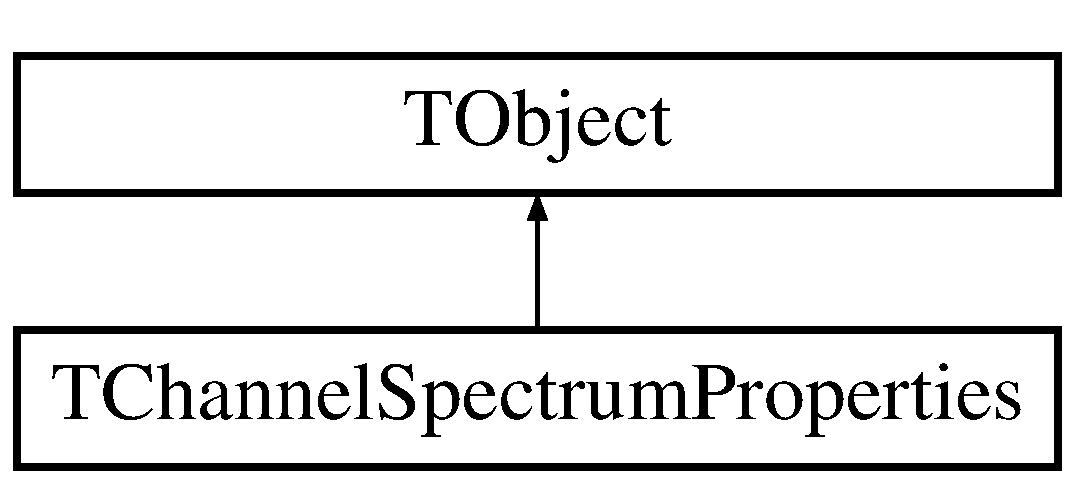
\includegraphics[height=2.000000cm]{class_t_channel_spectrum_properties}
\end{center}
\end{figure}
\subsection*{Public Member Functions}
\begin{DoxyCompactItemize}
\item 
\hyperlink{class_t_channel_spectrum_properties_ac1d3286952893fa565cbfd8227e84ff3}{T\-Channel\-Spectrum\-Properties} (Int\-\_\-t module=-\/1, Int\-\_\-t chip=-\/1, Int\-\_\-t channel=-\/1, Double\-\_\-t mean=0, Double\-\_\-t rms=0)
\begin{DoxyCompactList}\small\item\em The constructor. \end{DoxyCompactList}\item 
void \hyperlink{class_t_channel_spectrum_properties_a3ddfb6dfbbed5b502f1ddf5a40c387ba}{Set} (Int\-\_\-t module, Int\-\_\-t chip, Int\-\_\-t channel, Double\-\_\-t mean, Double\-\_\-t rms)
\begin{DoxyCompactList}\small\item\em Convenience function to set all member variables at once. \end{DoxyCompactList}\item 
\hyperlink{class_t_channel_spectrum_properties_a4b92e78edcf807e0353d5b059c55aa9c}{Class\-Def} (\hyperlink{class_t_channel_spectrum_properties}{T\-Channel\-Spectrum\-Properties}, 1)
\end{DoxyCompactItemize}
\subsection*{Data Fields}
\begin{DoxyCompactItemize}
\item 
Int\-\_\-t \hyperlink{class_t_channel_spectrum_properties_ae3cf44950a58087f83b1660648750619}{\-\_\-module}
\begin{DoxyCompactList}\small\item\em The readout module. \end{DoxyCompactList}\item 
Int\-\_\-t \hyperlink{class_t_channel_spectrum_properties_afdfd4c52a9b23cd7cd76dda75b595e27}{\-\_\-chip}
\begin{DoxyCompactList}\small\item\em The chip I\-D on this module. \end{DoxyCompactList}\item 
Int\-\_\-t \hyperlink{class_t_channel_spectrum_properties_a6bfd5e0b63e55aed4d1816a722f5c2e7}{\-\_\-channel}
\begin{DoxyCompactList}\small\item\em The channel I\-D within the chip. \end{DoxyCompactList}\item 
Double\-\_\-t \hyperlink{class_t_channel_spectrum_properties_a480a137b650eda8d36fb633de95259d1}{\-\_\-mean}
\begin{DoxyCompactList}\small\item\em The mean value of the spectrum. \end{DoxyCompactList}\item 
Double\-\_\-t \hyperlink{class_t_channel_spectrum_properties_a1eb2a743128d8069e0e962dfaaff3367}{\-\_\-rms}
\begin{DoxyCompactList}\small\item\em The rms of the spectrum. \end{DoxyCompactList}\end{DoxyCompactItemize}


\subsection{Detailed Description}
The \hyperlink{class_t_channel_spectrum_properties}{T\-Channel\-Spectrum\-Properties} class is used to store the channel information (slot, front\-End, module, chip) together with the spectrum properties (mean, rms) in a T\-Tree. 

Definition at line 11 of file T\-Channel\-Spectrum\-Properties.\-h.



\subsection{Constructor \& Destructor Documentation}
\hypertarget{class_t_channel_spectrum_properties_ac1d3286952893fa565cbfd8227e84ff3}{\index{T\-Channel\-Spectrum\-Properties@{T\-Channel\-Spectrum\-Properties}!T\-Channel\-Spectrum\-Properties@{T\-Channel\-Spectrum\-Properties}}
\index{T\-Channel\-Spectrum\-Properties@{T\-Channel\-Spectrum\-Properties}!TChannelSpectrumProperties@{T\-Channel\-Spectrum\-Properties}}
\subsubsection[{T\-Channel\-Spectrum\-Properties}]{\setlength{\rightskip}{0pt plus 5cm}T\-Channel\-Spectrum\-Properties\-::\-T\-Channel\-Spectrum\-Properties (
\begin{DoxyParamCaption}
\item[{Int\-\_\-t}]{module = {\ttfamily -\/1}, }
\item[{Int\-\_\-t}]{chip = {\ttfamily -\/1}, }
\item[{Int\-\_\-t}]{channel = {\ttfamily -\/1}, }
\item[{Double\-\_\-t}]{mean = {\ttfamily 0}, }
\item[{Double\-\_\-t}]{rms = {\ttfamily 0}}
\end{DoxyParamCaption}
)}}\label{class_t_channel_spectrum_properties_ac1d3286952893fa565cbfd8227e84ff3}


The constructor. 



Definition at line 5 of file T\-Channel\-Spectrum\-Properties.\-cxx.



\subsection{Member Function Documentation}
\hypertarget{class_t_channel_spectrum_properties_a4b92e78edcf807e0353d5b059c55aa9c}{\index{T\-Channel\-Spectrum\-Properties@{T\-Channel\-Spectrum\-Properties}!Class\-Def@{Class\-Def}}
\index{Class\-Def@{Class\-Def}!TChannelSpectrumProperties@{T\-Channel\-Spectrum\-Properties}}
\subsubsection[{Class\-Def}]{\setlength{\rightskip}{0pt plus 5cm}T\-Channel\-Spectrum\-Properties\-::\-Class\-Def (
\begin{DoxyParamCaption}
\item[{{\bf T\-Channel\-Spectrum\-Properties}}]{, }
\item[{1}]{}
\end{DoxyParamCaption}
)}}\label{class_t_channel_spectrum_properties_a4b92e78edcf807e0353d5b059c55aa9c}
\hypertarget{class_t_channel_spectrum_properties_a3ddfb6dfbbed5b502f1ddf5a40c387ba}{\index{T\-Channel\-Spectrum\-Properties@{T\-Channel\-Spectrum\-Properties}!Set@{Set}}
\index{Set@{Set}!TChannelSpectrumProperties@{T\-Channel\-Spectrum\-Properties}}
\subsubsection[{Set}]{\setlength{\rightskip}{0pt plus 5cm}void T\-Channel\-Spectrum\-Properties\-::\-Set (
\begin{DoxyParamCaption}
\item[{Int\-\_\-t}]{module, }
\item[{Int\-\_\-t}]{chip, }
\item[{Int\-\_\-t}]{channel, }
\item[{Double\-\_\-t}]{mean, }
\item[{Double\-\_\-t}]{rms}
\end{DoxyParamCaption}
)}}\label{class_t_channel_spectrum_properties_a3ddfb6dfbbed5b502f1ddf5a40c387ba}


Convenience function to set all member variables at once. 



Definition at line 11 of file T\-Channel\-Spectrum\-Properties.\-cxx.



References \-\_\-channel, \-\_\-chip, \-\_\-mean, \-\_\-module, and \-\_\-rms.



Referenced by Spectrum\-Properties\-Run\-Info\-::\-Spectrum\-Properties\-Run\-Info().



\subsection{Field Documentation}
\hypertarget{class_t_channel_spectrum_properties_a6bfd5e0b63e55aed4d1816a722f5c2e7}{\index{T\-Channel\-Spectrum\-Properties@{T\-Channel\-Spectrum\-Properties}!\-\_\-channel@{\-\_\-channel}}
\index{\-\_\-channel@{\-\_\-channel}!TChannelSpectrumProperties@{T\-Channel\-Spectrum\-Properties}}
\subsubsection[{\-\_\-channel}]{\setlength{\rightskip}{0pt plus 5cm}Int\-\_\-t T\-Channel\-Spectrum\-Properties\-::\-\_\-channel}}\label{class_t_channel_spectrum_properties_a6bfd5e0b63e55aed4d1816a722f5c2e7}


The channel I\-D within the chip. 



Definition at line 17 of file T\-Channel\-Spectrum\-Properties.\-h.



Referenced by Run\-Comparator\-::calculate\-Channel\-And\-Pedestal\-Corrected\-Mean(), Spectrum\-Properties\-Run\-Info\-::get\-Channels\-With\-Mean\-Cut(), Spectrum\-Properties\-Run\-Info\-::get\-Channels\-With\-R\-M\-S\-Cut(), Spectrum\-Properties\-Run\-Info\-::print(), Set(), and Spectrum\-Properties\-Run\-Info\-::\-Spectrum\-Properties\-Run\-Info().

\hypertarget{class_t_channel_spectrum_properties_afdfd4c52a9b23cd7cd76dda75b595e27}{\index{T\-Channel\-Spectrum\-Properties@{T\-Channel\-Spectrum\-Properties}!\-\_\-chip@{\-\_\-chip}}
\index{\-\_\-chip@{\-\_\-chip}!TChannelSpectrumProperties@{T\-Channel\-Spectrum\-Properties}}
\subsubsection[{\-\_\-chip}]{\setlength{\rightskip}{0pt plus 5cm}Int\-\_\-t T\-Channel\-Spectrum\-Properties\-::\-\_\-chip}}\label{class_t_channel_spectrum_properties_afdfd4c52a9b23cd7cd76dda75b595e27}


The chip I\-D on this module. 



Definition at line 16 of file T\-Channel\-Spectrum\-Properties.\-h.



Referenced by Run\-Comparator\-::calculate\-Channel\-And\-Pedestal\-Corrected\-Mean(), Spectrum\-Properties\-Run\-Info\-::get\-Channels\-With\-Mean\-Cut(), Spectrum\-Properties\-Run\-Info\-::get\-Channels\-With\-R\-M\-S\-Cut(), Spectrum\-Properties\-Run\-Info\-::print(), Set(), and Spectrum\-Properties\-Run\-Info\-::\-Spectrum\-Properties\-Run\-Info().

\hypertarget{class_t_channel_spectrum_properties_a480a137b650eda8d36fb633de95259d1}{\index{T\-Channel\-Spectrum\-Properties@{T\-Channel\-Spectrum\-Properties}!\-\_\-mean@{\-\_\-mean}}
\index{\-\_\-mean@{\-\_\-mean}!TChannelSpectrumProperties@{T\-Channel\-Spectrum\-Properties}}
\subsubsection[{\-\_\-mean}]{\setlength{\rightskip}{0pt plus 5cm}Double\-\_\-t T\-Channel\-Spectrum\-Properties\-::\-\_\-mean}}\label{class_t_channel_spectrum_properties_a480a137b650eda8d36fb633de95259d1}


The mean value of the spectrum. 



Definition at line 18 of file T\-Channel\-Spectrum\-Properties.\-h.



Referenced by Run\-Comparator\-::calculate\-Channel\-And\-Pedestal\-Corrected\-Mean(), Spectrum\-Properties\-Run\-Info\-::get\-Channels\-With\-Mean\-Cut(), Spectrum\-Properties\-Run\-Info\-::print(), and Set().

\hypertarget{class_t_channel_spectrum_properties_ae3cf44950a58087f83b1660648750619}{\index{T\-Channel\-Spectrum\-Properties@{T\-Channel\-Spectrum\-Properties}!\-\_\-module@{\-\_\-module}}
\index{\-\_\-module@{\-\_\-module}!TChannelSpectrumProperties@{T\-Channel\-Spectrum\-Properties}}
\subsubsection[{\-\_\-module}]{\setlength{\rightskip}{0pt plus 5cm}Int\-\_\-t T\-Channel\-Spectrum\-Properties\-::\-\_\-module}}\label{class_t_channel_spectrum_properties_ae3cf44950a58087f83b1660648750619}


The readout module. 



Definition at line 15 of file T\-Channel\-Spectrum\-Properties.\-h.



Referenced by Run\-Comparator\-::calculate\-Channel\-And\-Pedestal\-Corrected\-Mean(), Spectrum\-Properties\-Run\-Info\-::get\-Channels\-With\-Mean\-Cut(), Spectrum\-Properties\-Run\-Info\-::get\-Channels\-With\-R\-M\-S\-Cut(), Spectrum\-Properties\-Run\-Info\-::print(), Set(), and Spectrum\-Properties\-Run\-Info\-::\-Spectrum\-Properties\-Run\-Info().

\hypertarget{class_t_channel_spectrum_properties_a1eb2a743128d8069e0e962dfaaff3367}{\index{T\-Channel\-Spectrum\-Properties@{T\-Channel\-Spectrum\-Properties}!\-\_\-rms@{\-\_\-rms}}
\index{\-\_\-rms@{\-\_\-rms}!TChannelSpectrumProperties@{T\-Channel\-Spectrum\-Properties}}
\subsubsection[{\-\_\-rms}]{\setlength{\rightskip}{0pt plus 5cm}Double\-\_\-t T\-Channel\-Spectrum\-Properties\-::\-\_\-rms}}\label{class_t_channel_spectrum_properties_a1eb2a743128d8069e0e962dfaaff3367}


The rms of the spectrum. 



Definition at line 19 of file T\-Channel\-Spectrum\-Properties.\-h.



Referenced by Spectrum\-Properties\-Run\-Info\-::draw\-Get\-Dead\-Channels\-Plot(), Spectrum\-Properties\-Run\-Info\-::get\-Channels\-With\-R\-M\-S\-Cut(), Spectrum\-Properties\-Run\-Info\-::print(), and Set().



The documentation for this class was generated from the following files\-:\begin{DoxyCompactItemize}
\item 
\hyperlink{_t_channel_spectrum_properties_8h}{T\-Channel\-Spectrum\-Properties.\-h}\item 
\hyperlink{_t_channel_spectrum_properties_8cxx}{T\-Channel\-Spectrum\-Properties.\-cxx}\end{DoxyCompactItemize}

\chapter{File Documentation}
\hypertarget{_channel_expert_quality_8cxx}{\section{Channel\-Expert\-Quality.\-cxx File Reference}
\label{_channel_expert_quality_8cxx}\index{Channel\-Expert\-Quality.\-cxx@{Channel\-Expert\-Quality.\-cxx}}
}
{\ttfamily \#include \char`\"{}Channel\-Expert\-Quality.\-h\char`\"{}}\\*

\hypertarget{_channel_expert_quality_8h}{\section{Channel\-Expert\-Quality.\-h File Reference}
\label{_channel_expert_quality_8h}\index{Channel\-Expert\-Quality.\-h@{Channel\-Expert\-Quality.\-h}}
}
{\ttfamily \#include $<$Rtypes.\-h$>$}\\*
\subsection*{Data Structures}
\begin{DoxyCompactItemize}
\item 
class \hyperlink{class_channel_expert_quality}{Channel\-Expert\-Quality}
\begin{DoxyCompactList}\small\item\em A class holing the constants with define the detailed (expert) channel quality flags. \end{DoxyCompactList}\end{DoxyCompactItemize}

\hypertarget{create_bad_channels_list_8cpp}{\section{create\-Bad\-Channels\-List.\-cpp File Reference}
\label{create_bad_channels_list_8cpp}\index{create\-Bad\-Channels\-List.\-cpp@{create\-Bad\-Channels\-List.\-cpp}}
}
{\ttfamily \#include \char`\"{}Spectrum\-Properties\-Run\-Info.\-h\char`\"{}}\\*
{\ttfamily \#include \char`\"{}Channel\-Expert\-Quality.\-h\char`\"{}}\\*
{\ttfamily \#include $<$cstdlib$>$}\\*
{\ttfamily \#include $<$iostream$>$}\\*
{\ttfamily \#include $<$fstream$>$}\\*
{\ttfamily \#include $<$sstream$>$}\\*
{\ttfamily \#include $<$vector$>$}\\*
{\ttfamily \#include $<$T\-Graph.\-h$>$}\\*
{\ttfamily \#include $<$T\-Vector.\-h$>$}\\*
{\ttfamily \#include $<$T\-Canvas.\-h$>$}\\*
{\ttfamily \#include $<$T\-Legend.\-h$>$}\\*
{\ttfamily \#include $<$T\-Style.\-h$>$}\\*
{\ttfamily \#include $<$T\-Tree.\-h$>$}\\*
{\ttfamily \#include $<$T\-Directory.\-h$>$}\\*
{\ttfamily \#include $<$T\-R\-O\-O\-T.\-h$>$}\\*
{\ttfamily \#include $<$T\-File.\-h$>$}\\*
\subsection*{Functions}
\begin{DoxyCompactItemize}
\item 
void \hyperlink{create_bad_channels_list_8cpp_a6c144793f464f5d739a3f6409653db66}{print\-Usage} (void)
\item 
void \hyperlink{create_bad_channels_list_8cpp_a1f8e5e6ed3679bbb4b70c661327c4f94}{print\-Channel\-Status\-Map} (std\-::map$<$ int, int $>$ const \&channel\-Status\-Map, std\-::ostream \&s=std\-::cout)
\item 
int \hyperlink{create_bad_channels_list_8cpp_a0ddf1224851353fc92bfbff6f499fa97}{main} (int argc, char $\ast$argv\mbox{[}$\,$\mbox{]})
\end{DoxyCompactItemize}


\subsection{Function Documentation}
\hypertarget{create_bad_channels_list_8cpp_a0ddf1224851353fc92bfbff6f499fa97}{\index{create\-Bad\-Channels\-List.\-cpp@{create\-Bad\-Channels\-List.\-cpp}!main@{main}}
\index{main@{main}!createBadChannelsList.cpp@{create\-Bad\-Channels\-List.\-cpp}}
\subsubsection[{main}]{\setlength{\rightskip}{0pt plus 5cm}int main (
\begin{DoxyParamCaption}
\item[{int}]{argc, }
\item[{char $\ast$}]{argv\mbox{[}$\,$\mbox{]}}
\end{DoxyParamCaption}
)}}\label{create_bad_channels_list_8cpp_a0ddf1224851353fc92bfbff6f499fa97}


Definition at line 58 of file create\-Bad\-Channels\-List.\-cpp.



References Channel\-Expert\-Quality\-::dead, Spectrum\-Properties\-Run\-Info\-::get\-Global\-Channel\-Number(), Channel\-Expert\-Quality\-::high\-R\-M\-S, print\-Channel\-Status\-Map(), and print\-Usage().

\hypertarget{create_bad_channels_list_8cpp_a1f8e5e6ed3679bbb4b70c661327c4f94}{\index{create\-Bad\-Channels\-List.\-cpp@{create\-Bad\-Channels\-List.\-cpp}!print\-Channel\-Status\-Map@{print\-Channel\-Status\-Map}}
\index{print\-Channel\-Status\-Map@{print\-Channel\-Status\-Map}!createBadChannelsList.cpp@{create\-Bad\-Channels\-List.\-cpp}}
\subsubsection[{print\-Channel\-Status\-Map}]{\setlength{\rightskip}{0pt plus 5cm}void print\-Channel\-Status\-Map (
\begin{DoxyParamCaption}
\item[{std\-::map$<$ int, int $>$ const \&}]{channel\-Status\-Map, }
\item[{std\-::ostream \&}]{s = {\ttfamily std\-:\-:cout}}
\end{DoxyParamCaption}
)}}\label{create_bad_channels_list_8cpp_a1f8e5e6ed3679bbb4b70c661327c4f94}


Definition at line 39 of file create\-Bad\-Channels\-List.\-cpp.



References Spectrum\-Properties\-Run\-Info\-::\-Channel\-I\-D\-::\-\_\-channel, Spectrum\-Properties\-Run\-Info\-::\-Channel\-I\-D\-::\-\_\-chip, Spectrum\-Properties\-Run\-Info\-::\-Channel\-I\-D\-::\-\_\-module, and Spectrum\-Properties\-Run\-Info\-::get\-Channel\-I\-D().



Referenced by main().

\hypertarget{create_bad_channels_list_8cpp_a6c144793f464f5d739a3f6409653db66}{\index{create\-Bad\-Channels\-List.\-cpp@{create\-Bad\-Channels\-List.\-cpp}!print\-Usage@{print\-Usage}}
\index{print\-Usage@{print\-Usage}!createBadChannelsList.cpp@{create\-Bad\-Channels\-List.\-cpp}}
\subsubsection[{print\-Usage}]{\setlength{\rightskip}{0pt plus 5cm}void print\-Usage (
\begin{DoxyParamCaption}
\item[{void}]{}
\end{DoxyParamCaption}
)}}\label{create_bad_channels_list_8cpp_a6c144793f464f5d739a3f6409653db66}


Definition at line 19 of file create\-Bad\-Channels\-List.\-cpp.



Referenced by main().


\hypertarget{create_bad_channels_list_8dox}{\section{create\-Bad\-Channels\-List.\-dox File Reference}
\label{create_bad_channels_list_8dox}\index{create\-Bad\-Channels\-List.\-dox@{create\-Bad\-Channels\-List.\-dox}}
}

\hypertarget{create_spri_tree_8cpp}{\section{create\-Spri\-Tree.\-cpp File Reference}
\label{create_spri_tree_8cpp}\index{create\-Spri\-Tree.\-cpp@{create\-Spri\-Tree.\-cpp}}
}
{\ttfamily \#include \char`\"{}Spectrum\-Properties\-Run\-Info.\-h\char`\"{}}\\*
{\ttfamily \#include $<$cstdlib$>$}\\*
{\ttfamily \#include $<$iostream$>$}\\*
{\ttfamily \#include $<$fstream$>$}\\*
{\ttfamily \#include $<$sstream$>$}\\*
{\ttfamily \#include $<$vector$>$}\\*
{\ttfamily \#include $<$T\-Graph.\-h$>$}\\*
{\ttfamily \#include $<$T\-Vector.\-h$>$}\\*
{\ttfamily \#include $<$T\-Canvas.\-h$>$}\\*
{\ttfamily \#include $<$T\-Legend.\-h$>$}\\*
{\ttfamily \#include $<$T\-Style.\-h$>$}\\*
\subsection*{Functions}
\begin{DoxyCompactItemize}
\item 
void \hyperlink{create_spri_tree_8cpp_a6c144793f464f5d739a3f6409653db66}{print\-Usage} (void)
\item 
void \hyperlink{create_spri_tree_8cpp_a1f8e5e6ed3679bbb4b70c661327c4f94}{print\-Channel\-Status\-Map} (std\-::map$<$ int, int $>$ const \&channel\-Status\-Map, std\-::ostream \&s=std\-::cout)
\item 
int \hyperlink{create_spri_tree_8cpp_a0ddf1224851353fc92bfbff6f499fa97}{main} (int argc, char $\ast$argv\mbox{[}$\,$\mbox{]})
\end{DoxyCompactItemize}


\subsection{Function Documentation}
\hypertarget{create_spri_tree_8cpp_a0ddf1224851353fc92bfbff6f499fa97}{\index{create\-Spri\-Tree.\-cpp@{create\-Spri\-Tree.\-cpp}!main@{main}}
\index{main@{main}!createSpriTree.cpp@{create\-Spri\-Tree.\-cpp}}
\subsubsection[{main}]{\setlength{\rightskip}{0pt plus 5cm}int main (
\begin{DoxyParamCaption}
\item[{int}]{argc, }
\item[{char $\ast$}]{argv\mbox{[}$\,$\mbox{]}}
\end{DoxyParamCaption}
)}}\label{create_spri_tree_8cpp_a0ddf1224851353fc92bfbff6f499fa97}


Definition at line 64 of file create\-Spri\-Tree.\-cpp.



References Spectrum\-Properties\-Run\-Info\-::get\-Spectrum\-Properties\-Tree(), and print\-Usage().

\hypertarget{create_spri_tree_8cpp_a1f8e5e6ed3679bbb4b70c661327c4f94}{\index{create\-Spri\-Tree.\-cpp@{create\-Spri\-Tree.\-cpp}!print\-Channel\-Status\-Map@{print\-Channel\-Status\-Map}}
\index{print\-Channel\-Status\-Map@{print\-Channel\-Status\-Map}!createSpriTree.cpp@{create\-Spri\-Tree.\-cpp}}
\subsubsection[{print\-Channel\-Status\-Map}]{\setlength{\rightskip}{0pt plus 5cm}void print\-Channel\-Status\-Map (
\begin{DoxyParamCaption}
\item[{std\-::map$<$ int, int $>$ const \&}]{channel\-Status\-Map, }
\item[{std\-::ostream \&}]{s = {\ttfamily std\-:\-:cout}}
\end{DoxyParamCaption}
)}}\label{create_spri_tree_8cpp_a1f8e5e6ed3679bbb4b70c661327c4f94}


Definition at line 45 of file create\-Spri\-Tree.\-cpp.



References Spectrum\-Properties\-Run\-Info\-::\-Channel\-I\-D\-::\-\_\-channel, Spectrum\-Properties\-Run\-Info\-::\-Channel\-I\-D\-::\-\_\-chip, Spectrum\-Properties\-Run\-Info\-::\-Channel\-I\-D\-::\-\_\-module, and Spectrum\-Properties\-Run\-Info\-::get\-Channel\-I\-D().

\hypertarget{create_spri_tree_8cpp_a6c144793f464f5d739a3f6409653db66}{\index{create\-Spri\-Tree.\-cpp@{create\-Spri\-Tree.\-cpp}!print\-Usage@{print\-Usage}}
\index{print\-Usage@{print\-Usage}!createSpriTree.cpp@{create\-Spri\-Tree.\-cpp}}
\subsubsection[{print\-Usage}]{\setlength{\rightskip}{0pt plus 5cm}void print\-Usage (
\begin{DoxyParamCaption}
\item[{void}]{}
\end{DoxyParamCaption}
)}}\label{create_spri_tree_8cpp_a6c144793f464f5d739a3f6409653db66}


Definition at line 28 of file create\-Spri\-Tree.\-cpp.


\hypertarget{examples_8dox}{\section{examples.\-dox File Reference}
\label{examples_8dox}\index{examples.\-dox@{examples.\-dox}}
}

\hypertarget{installation_8dox}{\section{installation.\-dox File Reference}
\label{installation_8dox}\index{installation.\-dox@{installation.\-dox}}
}

\hypertarget{_link_def_8h}{\section{Link\-Def.\-h File Reference}
\label{_link_def_8h}\index{Link\-Def.\-h@{Link\-Def.\-h}}
}

\hypertarget{_mainpage_8dox}{\section{Mainpage.\-dox File Reference}
\label{_mainpage_8dox}\index{Mainpage.\-dox@{Mainpage.\-dox}}
}

\hypertarget{_module_type_8cxx}{\section{Module\-Type.\-cxx File Reference}
\label{_module_type_8cxx}\index{Module\-Type.\-cxx@{Module\-Type.\-cxx}}
}
{\ttfamily \#include \char`\"{}Module\-Type.\-h\char`\"{}}\\*

\hypertarget{_module_type_8h}{\section{Module\-Type.\-h File Reference}
\label{_module_type_8h}\index{Module\-Type.\-h@{Module\-Type.\-h}}
}
\subsection*{Data Structures}
\begin{DoxyCompactItemize}
\item 
class \hyperlink{class_module_type}{Module\-Type}
\begin{DoxyCompactList}\small\item\em A class to define the different module types. \end{DoxyCompactList}\end{DoxyCompactItemize}

\hypertarget{root_lib_8dox}{\section{root\-Lib.\-dox File Reference}
\label{root_lib_8dox}\index{root\-Lib.\-dox@{root\-Lib.\-dox}}
}

\hypertarget{_run_comparator_8cxx}{\section{Run\-Comparator.\-cxx File Reference}
\label{_run_comparator_8cxx}\index{Run\-Comparator.\-cxx@{Run\-Comparator.\-cxx}}
}
{\ttfamily \#include \char`\"{}Run\-Comparator.\-h\char`\"{}}\\*
{\ttfamily \#include $<$iterator$>$}\\*
{\ttfamily \#include $<$T\-Vector\-D.\-h$>$}\\*
{\ttfamily \#include $<$T\-String.\-h$>$}\\*

\hypertarget{_run_comparator_8h}{\section{Run\-Comparator.\-h File Reference}
\label{_run_comparator_8h}\index{Run\-Comparator.\-h@{Run\-Comparator.\-h}}
}
{\ttfamily \#include \char`\"{}T\-Channel\-Spectrum\-Properties.\-h\char`\"{}}\\*
{\ttfamily \#include \char`\"{}Spectrum\-Properties\-Run\-Info.\-h\char`\"{}}\\*
{\ttfamily \#include $<$map$>$}\\*
{\ttfamily \#include $<$set$>$}\\*
{\ttfamily \#include $<$vector$>$}\\*
{\ttfamily \#include $<$cfloat$>$}\\*
{\ttfamily \#include $<$T\-H1\-D.\-h$>$}\\*
{\ttfamily \#include $<$T\-Graph.\-h$>$}\\*
\subsection*{Data Structures}
\begin{DoxyCompactItemize}
\item 
class \hyperlink{class_run_comparator}{Run\-Comparator}
\begin{DoxyCompactList}\small\item\em A class to facilitate the comparison of two runs. \end{DoxyCompactList}\end{DoxyCompactItemize}

\hypertarget{_simple_mapper_8cxx}{\section{Simple\-Mapper.\-cxx File Reference}
\label{_simple_mapper_8cxx}\index{Simple\-Mapper.\-cxx@{Simple\-Mapper.\-cxx}}
}
{\ttfamily \#include \char`\"{}Simple\-Mapper.\-h\char`\"{}}\\*
{\ttfamily \#include \char`\"{}Module\-Type.\-h\char`\"{}}\\*
{\ttfamily \#include $<$iostream$>$}\\*
{\ttfamily \#include $<$fstream$>$}\\*
{\ttfamily \#include $<$string$>$}\\*
\subsection*{Macros}
\begin{DoxyCompactItemize}
\item 
\#define \hyperlink{_simple_mapper_8cxx_a8a66270365fd38183668e1b7d3865c48}{A\-H\-C\-A\-L\-\_\-\-M\-A\-X\-\_\-\-L\-A\-Y\-E\-R\-S}~38
\end{DoxyCompactItemize}


\subsection{Macro Definition Documentation}
\hypertarget{_simple_mapper_8cxx_a8a66270365fd38183668e1b7d3865c48}{\index{Simple\-Mapper.\-cxx@{Simple\-Mapper.\-cxx}!A\-H\-C\-A\-L\-\_\-\-M\-A\-X\-\_\-\-L\-A\-Y\-E\-R\-S@{A\-H\-C\-A\-L\-\_\-\-M\-A\-X\-\_\-\-L\-A\-Y\-E\-R\-S}}
\index{A\-H\-C\-A\-L\-\_\-\-M\-A\-X\-\_\-\-L\-A\-Y\-E\-R\-S@{A\-H\-C\-A\-L\-\_\-\-M\-A\-X\-\_\-\-L\-A\-Y\-E\-R\-S}!SimpleMapper.cxx@{Simple\-Mapper.\-cxx}}
\subsubsection[{A\-H\-C\-A\-L\-\_\-\-M\-A\-X\-\_\-\-L\-A\-Y\-E\-R\-S}]{\setlength{\rightskip}{0pt plus 5cm}\#define A\-H\-C\-A\-L\-\_\-\-M\-A\-X\-\_\-\-L\-A\-Y\-E\-R\-S~38}}\label{_simple_mapper_8cxx_a8a66270365fd38183668e1b7d3865c48}


Definition at line 8 of file Simple\-Mapper.\-cxx.



Referenced by Simple\-Mapper\-::\-Simple\-Mapper().


\hypertarget{_simple_mapper_8h}{\section{Simple\-Mapper.\-h File Reference}
\label{_simple_mapper_8h}\index{Simple\-Mapper.\-h@{Simple\-Mapper.\-h}}
}
{\ttfamily \#include $<$string$>$}\\*
{\ttfamily \#include $<$map$>$}\\*
\subsection*{Data Structures}
\begin{DoxyCompactItemize}
\item 
class \hyperlink{class_simple_mapper}{Simple\-Mapper}
\begin{DoxyCompactList}\small\item\em The \hyperlink{class_simple_mapper}{Simple\-Mapper} helper class reads in the A\-H\-C.\-cfg text file and provides the mapping (slot, frontend) -\/$>$ (module, chip) \end{DoxyCompactList}\item 
struct \hyperlink{struct_simple_mapper_1_1_module_description}{Simple\-Mapper\-::\-Module\-Description}
\begin{DoxyCompactList}\small\item\em Internal helper struct for the value\-: a module description consisting of. \end{DoxyCompactList}\end{DoxyCompactItemize}

\hypertarget{_spectrum_properties_run_info_8cxx}{\section{Spectrum\-Properties\-Run\-Info.\-cxx File Reference}
\label{_spectrum_properties_run_info_8cxx}\index{Spectrum\-Properties\-Run\-Info.\-cxx@{Spectrum\-Properties\-Run\-Info.\-cxx}}
}
{\ttfamily \#include \char`\"{}Spectrum\-Properties\-Run\-Info.\-h\char`\"{}}\\*
{\ttfamily \#include \char`\"{}Simple\-Mapper.\-h\char`\"{}}\\*
{\ttfamily \#include $<$string$>$}\\*
{\ttfamily \#include $<$iostream$>$}\\*
{\ttfamily \#include $<$fstream$>$}\\*
{\ttfamily \#include $<$T\-File.\-h$>$}\\*
{\ttfamily \#include $<$T\-Iterator.\-h$>$}\\*
{\ttfamily \#include $<$T\-Collection.\-h$>$}\\*
{\ttfamily \#include $<$T\-Tree.\-h$>$}\\*
{\ttfamily \#include $<$T\-H1\-D.\-h$>$}\\*
{\ttfamily \#include $<$T\-R\-O\-O\-T.\-h$>$}\\*
{\ttfamily \#include $<$T\-Key.\-h$>$}\\*
\subsection*{Macros}
\begin{DoxyCompactItemize}
\item 
\#define \hyperlink{_spectrum_properties_run_info_8cxx_a0a3abbca80bc98e7abcb3ae73abe0f14}{M\-A\-X\-\_\-\-I\-T\-E\-R\-A\-T\-I\-O\-N\-S}~10
\end{DoxyCompactItemize}


\subsection{Macro Definition Documentation}
\hypertarget{_spectrum_properties_run_info_8cxx_a0a3abbca80bc98e7abcb3ae73abe0f14}{\index{Spectrum\-Properties\-Run\-Info.\-cxx@{Spectrum\-Properties\-Run\-Info.\-cxx}!M\-A\-X\-\_\-\-I\-T\-E\-R\-A\-T\-I\-O\-N\-S@{M\-A\-X\-\_\-\-I\-T\-E\-R\-A\-T\-I\-O\-N\-S}}
\index{M\-A\-X\-\_\-\-I\-T\-E\-R\-A\-T\-I\-O\-N\-S@{M\-A\-X\-\_\-\-I\-T\-E\-R\-A\-T\-I\-O\-N\-S}!SpectrumPropertiesRunInfo.cxx@{Spectrum\-Properties\-Run\-Info.\-cxx}}
\subsubsection[{M\-A\-X\-\_\-\-I\-T\-E\-R\-A\-T\-I\-O\-N\-S}]{\setlength{\rightskip}{0pt plus 5cm}\#define M\-A\-X\-\_\-\-I\-T\-E\-R\-A\-T\-I\-O\-N\-S~10}}\label{_spectrum_properties_run_info_8cxx_a0a3abbca80bc98e7abcb3ae73abe0f14}


Definition at line 16 of file Spectrum\-Properties\-Run\-Info.\-cxx.



Referenced by Spectrum\-Properties\-Run\-Info\-::\-Spectrum\-Properties\-Run\-Info().


\hypertarget{_spectrum_properties_run_info_8h}{\section{Spectrum\-Properties\-Run\-Info.\-h File Reference}
\label{_spectrum_properties_run_info_8h}\index{Spectrum\-Properties\-Run\-Info.\-h@{Spectrum\-Properties\-Run\-Info.\-h}}
}
{\ttfamily \#include $<$T\-Tree.\-h$>$}\\*
{\ttfamily \#include $<$T\-File.\-h$>$}\\*
{\ttfamily \#include $<$T\-String.\-h$>$}\\*
{\ttfamily \#include $<$T\-H\-Stack.\-h$>$}\\*
{\ttfamily \#include \char`\"{}T\-Channel\-Spectrum\-Properties.\-h\char`\"{}}\\*
{\ttfamily \#include \char`\"{}Simple\-Mapper.\-h\char`\"{}}\\*
{\ttfamily \#include $<$vector$>$}\\*
{\ttfamily \#include $<$string$>$}\\*
{\ttfamily \#include $<$T\-H1\-D.\-h$>$}\\*
{\ttfamily \#include $<$iostream$>$}\\*
{\ttfamily \#include $<$cfloat$>$}\\*
{\ttfamily \#include \char`\"{}Module\-Type.\-h\char`\"{}}\\*
\subsection*{Data Structures}
\begin{DoxyCompactItemize}
\item 
class \hyperlink{class_spectrum_properties_run_info}{Spectrum\-Properties\-Run\-Info}
\begin{DoxyCompactList}\small\item\em The \hyperlink{class_spectrum_properties_run_info}{Spectrum\-Properties\-Run\-Info} is a utility class to access the spectrum properties for all channels of one specific run. \end{DoxyCompactList}\item 
class \hyperlink{class_spectrum_properties_run_info_1_1_channel_i_d}{Spectrum\-Properties\-Run\-Info\-::\-Channel\-I\-D}
\begin{DoxyCompactList}\small\item\em A channel identifier helper class. The key in the map. \end{DoxyCompactList}\end{DoxyCompactItemize}

\hypertarget{_t_channel_spectrum_properties_8cxx}{\section{T\-Channel\-Spectrum\-Properties.\-cxx File Reference}
\label{_t_channel_spectrum_properties_8cxx}\index{T\-Channel\-Spectrum\-Properties.\-cxx@{T\-Channel\-Spectrum\-Properties.\-cxx}}
}
{\ttfamily \#include \char`\"{}T\-Channel\-Spectrum\-Properties.\-h\char`\"{}}\\*

\hypertarget{_t_channel_spectrum_properties_8h}{\section{T\-Channel\-Spectrum\-Properties.\-h File Reference}
\label{_t_channel_spectrum_properties_8h}\index{T\-Channel\-Spectrum\-Properties.\-h@{T\-Channel\-Spectrum\-Properties.\-h}}
}
{\ttfamily \#include $<$T\-Object.\-h$>$}\\*
\subsection*{Data Structures}
\begin{DoxyCompactItemize}
\item 
class \hyperlink{class_t_channel_spectrum_properties}{T\-Channel\-Spectrum\-Properties}
\begin{DoxyCompactList}\small\item\em The \hyperlink{class_t_channel_spectrum_properties}{T\-Channel\-Spectrum\-Properties} class is used to store the channel information (slot, front\-End, module, chip) together with the spectrum properties (mean, rms) in a T\-Tree. \end{DoxyCompactList}\end{DoxyCompactItemize}

\hypertarget{test_run_comparator_8cpp}{\section{test\-Run\-Comparator.\-cpp File Reference}
\label{test_run_comparator_8cpp}\index{test\-Run\-Comparator.\-cpp@{test\-Run\-Comparator.\-cpp}}
}
{\ttfamily \#include \char`\"{}Spectrum\-Properties\-Run\-Info.\-h\char`\"{}}\\*
{\ttfamily \#include \char`\"{}Run\-Comparator.\-h\char`\"{}}\\*
{\ttfamily \#include \char`\"{}T\-Graph.\-h\char`\"{}}\\*
{\ttfamily \#include \char`\"{}T\-H1\-D.\-h\char`\"{}}\\*
{\ttfamily \#include $<$unistd.\-h$>$}\\*
\subsection*{Functions}
\begin{DoxyCompactItemize}
\item 
int \hyperlink{test_run_comparator_8cpp_ae66f6b31b5ad750f1fe042a706a4e3d4}{main} ()
\end{DoxyCompactItemize}


\subsection{Function Documentation}
\hypertarget{test_run_comparator_8cpp_ae66f6b31b5ad750f1fe042a706a4e3d4}{\index{test\-Run\-Comparator.\-cpp@{test\-Run\-Comparator.\-cpp}!main@{main}}
\index{main@{main}!testRunComparator.cpp@{test\-Run\-Comparator.\-cpp}}
\subsubsection[{main}]{\setlength{\rightskip}{0pt plus 5cm}int main (
\begin{DoxyParamCaption}
{}
\end{DoxyParamCaption}
)}}\label{test_run_comparator_8cpp_ae66f6b31b5ad750f1fe042a706a4e3d4}


Definition at line 6 of file test\-Run\-Comparator.\-cpp.



References Run\-Comparator\-::calculate\-Channel\-And\-Pedestal\-Corrected\-Mean(), Run\-Comparator\-::get\-Graph(), Run\-Comparator\-::get\-X\-Axis\-Histo(), Run\-Comparator\-::get\-Y\-Axis\-Histo(), and Run\-Comparator\-::prepare\-Graph().


\hypertarget{test_simple_mapper_8cpp}{\section{test\-Simple\-Mapper.\-cpp File Reference}
\label{test_simple_mapper_8cpp}\index{test\-Simple\-Mapper.\-cpp@{test\-Simple\-Mapper.\-cpp}}
}
{\ttfamily \#include \char`\"{}Simple\-Mapper.\-h\char`\"{}}\\*
{\ttfamily \#include $<$iostream$>$}\\*
{\ttfamily \#include $<$string$>$}\\*
\subsection*{Functions}
\begin{DoxyCompactItemize}
\item 
int \hyperlink{test_simple_mapper_8cpp_a0ddf1224851353fc92bfbff6f499fa97}{main} (int argc, char $\ast$argv\mbox{[}$\,$\mbox{]})
\end{DoxyCompactItemize}


\subsection{Function Documentation}
\hypertarget{test_simple_mapper_8cpp_a0ddf1224851353fc92bfbff6f499fa97}{\index{test\-Simple\-Mapper.\-cpp@{test\-Simple\-Mapper.\-cpp}!main@{main}}
\index{main@{main}!testSimpleMapper.cpp@{test\-Simple\-Mapper.\-cpp}}
\subsubsection[{main}]{\setlength{\rightskip}{0pt plus 5cm}int main (
\begin{DoxyParamCaption}
\item[{int}]{argc, }
\item[{char $\ast$}]{argv\mbox{[}$\,$\mbox{]}}
\end{DoxyParamCaption}
)}}\label{test_simple_mapper_8cpp_a0ddf1224851353fc92bfbff6f499fa97}


Definition at line 5 of file test\-Simple\-Mapper.\-cpp.



References Simple\-Mapper\-::print().


%--- End generated contents ---

% Index
\newpage
\phantomsection
\addcontentsline{toc}{part}{Index}
\printindex

\end{document}
